%%%%%%%%%%%%%%%%%%%%%%%%%%%%%%%%%%%%%%%%%%%%%%%%%%%%%%%%%%%%%%%%%%%%%%%%%
%  Zawarto: Gwny plik szablonu pracy dyplomowej (magisterskiej/inynierskiej). 
%  Opracowa: Tomasz Kubik <tomasz.kubik@pwr.edu.pl>
%  Data: 9 lutego 2021
%  Wersja: 0.5
%  Wymagania: dedykowany do kompilatora pdflatex.
%%%%%%%%%%%%%%%%%%%%%%%%%%%%%%%%%%%%%%%%%%%%%%%%%%%%%%%%%%%%%%%%%%%%%%%%%

\documentclass[a4paper,onecolumn,oneside,12pt,extrafontsizes]{memoir}
%  W celu przygotowania wydruku  do archiwum mona:
%  a) przygotowa pdf, w ktrym dwie strony zostan wstawione na jedn fizyczn stron i taki dokument wydrukowa dwustronnie (podejcie zalecane)
%
%   Taki dokument mona przygotowa poprzez
%   - wydruk z Adobe Acrobat Reader z opcj "Wiele" - sekcja "Rozmiar i obsuga stron"
%   - wykorzystanie narzdzi psutils
%
%      Windows (zakadajc, e w dystrybucji MiKTeX jest pakiet miktex-psutils-bin-x64-2.9):
%        "c:\Program Files\MiKTeX 2.9\miktex\bin\x64\pdf2ps.exe" Dyplom.pdf Dyplom.ps
%        "c:\Program Files\MiKTeX 2.9\miktex\bin\x64\psnup.exe" -2 Dyplom.ps Dyplom2.ps
%        "c:\Program Files\MiKTeX 2.9\miktex\bin\x64\ps2pdf.exe" Dyplom2.ps Dyplom2.pdf
%        Del Dyplom2.ps Dyplom.ps
%
%     Linux:
%        pdf2ps Dyplom.pdf - | psnup -2 | ps2pdf - Dyplom2.pdf
%
%  b) przekomplilowa dokument zmniejszajc czcionk (podejcie niezalecane, bo zmienia formatowanie dokumentu)
%
%    Do tego wystarczy posuy si poniszymi komendami (zamiast documentclass z pierwszej linijki):
%   \documentclass[a4paper,onecolumn,twoside,10pt]{memoir} 
%   \renewcommand{\normalsize}{\fontsize{8pt}{10pt}\selectfont}

%\usepackage[cp1250]{inputenc} % Prosz zostawi, jeli kodowanie edytowanych plikw to cp1250 
\usepackage[utf8]{inputenc} % Prosz uy zamiast powyszego, jeli kodowanie edytowanych plikw to UTF8
\usepackage[T1]{fontenc}
\usepackage[english,polish]{babel} % Tutaj wana jest kolejno atrybutw (dla pracy po polsku polish powinno by na kocu)
%\DisemulatePackage{setspace}
\usepackage{setspace}
\usepackage{geometry}
\usepackage{color,calc}
%\usepackage{soul} % pakiet z komendami do podkrelania, przekrelania, podwietlania tekstu (raczej niepotrzebny)

\usepackage{ebgaramond} % pakiet z czcionkami garamond, potrzebny tylko do strony tytuowej, musi wystpi przed pakietem tgtermes

%% Aby uzyska polskie literki w pdfie (a nie zlepki) korzystamy z pakietu czcionek tgterms. 
%% W pakiecie tym s zdefiniowane klony czcionek Times o ksztatach: normalny, pogrubiony, italic, italic pogrubiony.
%% W pakiecie tym brakuje czcionki o ksztacie: slanted (podobny do italic). 
%% Jeli w dokumencie gdzie zostanie zastosowana czcionka slanted (np. po uyciu komendy \textsl{}), to
%% latex dokona podstawienia na czcionk standardow i zgosi to w ostrzeeniu (warningu).
%% Ponadto tgtermes to czcionka do tekstu. Wszelkie matematyczne wzory bd sformatowane domyln czcionk do wzorw.
%% Jeli wzory maj by sformatowane z wykorzystaniem innych czcionek, trzeba to jawnie zadeklarowa.

%% Po zainstalowaniu pakietu tgtermes moe bdzie trzeba zauktualizowa informacje 
%% o dostpnych fontach oraz mapy. Mona to zrobi z konsoli (jako administrator)
%% initexmf --admin --update-fndb
%% initexmf --admin --mkmaps

\usepackage{tgtermes}   
\renewcommand*\ttdefault{txtt}



\usepackage{multicol} % pakiet umoliwiajcy stworzenie wielokolumnowego tekstu
%%%%%%%%%%%%%%%%%%%%%%%%%%%%%%%%%%%%%%%%%%%%%%%%%%%
%% Pakiety do formatowania tabel
%%%%%%%%%%%%%%%%%%%%%%%%%%%%%%%%%%%%%%%%%%%%%%%%%%%
\usepackage{tabularx}
% Prosz uywa tylko tabularx. Innych pakietw prosz nie stosowa !!!
% Dokument na pewno da si zredagowa bez ich uycia.
\usepackage{longtable}
%\usepackage{ltxtable}
%\usepackage{tabulary}

%%%%%%%%%%%%%%%%%%%%%%%%%%%%%%%%%%%%%%%%%%%%%%%%%%%
%% Pakiet do wstawiania fragmentw kodu
%%%%%%%%%%%%%%%%%%%%%%%%%%%%%%%%%%%%%%%%%%%%%%%%%%%
\usepackage{listings} 
\usepackage{xpatch}
\makeatletter
\xpatchcmd\l@lstlisting{1.5em}{0em}{}{}
\makeatother
% Pakiet dostarcza otoczenia lstlisting. Jest ono wysoce konfigurowalne. 
% Konfigurowa mona indywidualnie kady z listingw lub globalnie, w poleceniu \lstset{}.

% Zalecane jest, by kod rdowy by wyprowadzany z uyciem czcionki maszynowej \ttfamily
% Poniewa kod rdowy, nawet po obciciu do interesujcych fragmentw, bywa obszerny, naley zmniejszy czcionk.
% Zalecane jest \small (dla krtkich fragmentw) oraz \footnotesize (dla duszych fragmentw).

% Ponadto podczas konfiguracji mona zadeklarowa sposb numerowania linii. Numerowanie linii zalecane jest jednak 
% tylko w przypadkach, gdy w opisie zamieszczonym w tekcie znajduj si jakie odwoania do konkretnych linii.
% Jeli w opisie nie ma takich odwoa, numerowanie linii jest zbdne. Prosz wtedy go nie stosowa.
% Przy wczaniu numerowania linii naley zwrci uwag na to, gdzie pojawi si te numery.
% Bez zmiany dodatkowych parametrw pojawiaj si one na marginesie strony (co jest nieporzdane).

\lstset{
  basicstyle=\small\ttfamily, % lub basicstyle=\footnotesize\ttfamily
  %%columns=fullflexible,
	%%showstringspaces=false,
	%%showspaces=false,
  breaklines=true,
  postbreak=\mbox{\textcolor{red}{$\hookrightarrow$}\space}, 
  %%numbers=left,  % ta i ponisze linie dotycz ustawienia numerowania i sposobu jego wyprowadzania
  %%firstnumber=1, 
  %%numberfirstline=true, 
	%%xleftmargin=17pt,
  %%framexleftmargin=17pt,
  %%framexrightmargin=5pt,
  %%framexbottommargin=4pt,
	belowskip=.5\baselineskip
}

% Jeli edytowany plik nie jest w kodowaniu cp1250, to jest problem z polskimi znakami wystpujcymi we wstawianym kodzie.
% Dlatego podczas pracy na plikach w kodowaniu UTF-8 trzeba zadeklarowa mapowanie jak niej (wystarczy odmarkowa).
% Niestety, jak si zastosuje to mapowanie mog pojawi si problemy z podwietlaniem skadni (patrz dalej).
%%\lstset{literate=%-
%%{}{{\k{a}}}1 {}{{\'c}}1 {}{{\k{e}}}1 {}{{\l{}}}1 {}{{\'n}}1 {}{{\'o}}1 {}{{\'s}}1 {}{{\.z}}1 {}{{\'z}}1 {}{{\k{A}}}1 {}{{\'C}}1 {}{{\k{E}}}1 {}{{\L{}}}1 {}{{\'N}}1 {}{{\'O}}1 {}{{\'S}}1 {}{{\.Z}}1 {}{{\'Z}}1 
    %%{}{{\"O}}1
    %%{}{{\"A}}1
    %%{}{{\"U}}1
    %%{}{{\ss}}1
    %%{}{{\"u}}1
    %%{}{{\"a}}1
    %%{}{{\"o}}1
    %%{~}{{\textasciitilde}}1
		%%{}{{{\textemdash} }}1
%%}%{\ \ }{{\ }}1}


%% lstlisting pozwala na ostylowania podwietlania skadni wybranych jzykw.
%% Dziaa to na zasadzie zdefiniowania sw kluczowych oraz sposobu ich wywietlania.
%% Poniewa jest to prosty mechanizm, czasem trudno osign takie efekty, jakie daj narzdzia IDE. 
%% Jednak w wikszoci przypadku osigane rezutlaty s zadowalajce.
%%\lstloadlanguages{% Check Dokumentation for further languages ...
%%C,
%%C++,
%%csh,
%%Java
%%}


%% lstlisting obsuguje domylnie kilka najpopularniejszych jzykw.
%% Inne jzyki musz by dodefiniowane. Poniej podano przykady definicji jzykw i styli.

\definecolor{lightgray}{rgb}{.9,.9,.9}
\definecolor{darkgray}{rgb}{.4,.4,.4}
\definecolor{purple}{rgb}{0.65, 0.12, 0.82}
\definecolor{javared}{rgb}{0.6,0,0} % for strings
\definecolor{javagreen}{rgb}{0.25,0.5,0.35} % comments
\definecolor{javapurple}{rgb}{0.5,0,0.35} % keywords
\definecolor{javadocblue}{rgb}{0.25,0.35,0.75} % javadoc
 
\lstdefinelanguage{JavaScript}{ 
	keywords={typeof, new, true, false, catch, function, return, null, catch, switch, var, if, in, while, do, else, case, break},
	keywordstyle=\color{blue}\bfseries,
	ndkeywords={class, export, boolean, throw, implements, import, this},
	ndkeywordstyle=\color{darkgray}\bfseries,
	identifierstyle=\color{black},
	sensitive=false,
	comment=[l]{//},
	morecomment=[s]{/*}{*/},
	commentstyle=\color{purple}\ttfamily,
	stringstyle=\color{red}\ttfamily,
	morestring=[b]',
	morestring=[b]"
}
\lstdefinestyle{JavaScriptStyle}{
	language=JavaScript,
	commentstyle=\color{javagreen}, % niestety, jeli w linii komentarza pojawi si sowa kluczowe, to zostan pokolorowane
	backgroundcolor=,%\color{lightgray}, % mona ustwi kolor ta, ale jest to niezalecane
	extendedchars=true,
	basicstyle=\footnotesize\ttfamily,
	showstringspaces=false,
	showspaces=false,
	numbers=none,%left,
	numberstyle=\footnotesize,
	numbersep=9pt,
	tabsize=2,
	breaklines=true,
	showtabs=false,
	captionpos=t
}

\lstdefinestyle{JavaStyle}{
basicstyle=\footnotesize\ttfamily,
keywordstyle=\color{javapurple}\bfseries,
stringstyle=\color{javared},
commentstyle=\color{javagreen},
morecomment=[s][\color{javadocblue}]{/**}{*/},
numbers=none,%left,
numberstyle=\tiny\color{black},
stepnumber=2,
numbersep=10pt,
tabsize=4,
showspaces=false,
showstringspaces=false,
captionpos=t
}

\definecolor{pblue}{rgb}{0.13,0.13,1}
\definecolor{pgreen}{rgb}{0,0.5,0}
\definecolor{pred}{rgb}{0.9,0,0}
\definecolor{pgrey}{rgb}{0.46,0.45,0.48}
\definecolor{dark-grey}{rgb}{0.4,0.4,0.4}
% styl json
\newcommand\JSONnumbervaluestyle{\color{blue}}
\newcommand\JSONstringvaluestyle{\color{red}}

\newif\ifcolonfoundonthisline

\makeatletter

\lstdefinestyle{json-style}  
{
	showstringspaces    = false,
	keywords            = {false,true},
	alsoletter          = 0123456789.,
	morestring          = [s]{"}{"},
	stringstyle         = \ifcolonfoundonthisline\JSONstringvaluestyle\fi,
	MoreSelectCharTable =%
	\lst@DefSaveDef{`:}\colon@json{\processColon@json},
	basicstyle          = \footnotesize\ttfamily,
	keywordstyle        = \ttfamily\bfseries,
	numbers				= left, % zamarkowa, jeli numeracja linii jest niepotrzebna
	numberstyle={\footnotesize\ttfamily\color{dark-grey}},
	xleftmargin			= 2em % zamarkowa, jeli numeracja linii jest niepotrzebna
}

\newcommand\processColon@json{%
	\colon@json%
	\ifnum\lst@mode=\lst@Pmode%
	\global\colonfoundonthislinetrue%
	\fi
}

\lst@AddToHook{Output}{%
	\ifcolonfoundonthisline%
	\ifnum\lst@mode=\lst@Pmode%
	\def\lst@thestyle{\JSONnumbervaluestyle}%
	\fi
	\fi
	\lsthk@DetectKeywords% 
}

\lst@AddToHook{EOL}%
{\global\colonfoundonthislinefalse}

\makeatother

%%\definecolor{red}{rgb}{0.6,0,0} % for strings
%%\definecolor{blue}{rgb}{0,0,0.6}
%%\definecolor{green}{rgb}{0,0.8,0}
%%\definecolor{cyan}{rgb}{0.0,0.6,0.6}
%%
%%\lstdefinestyle{sqlstyle}{
%%language=SQL,
%%basicstyle=\footnotesize\ttfamily, 
%%numbers=left, 
%%numberstyle=\tiny, 
%%numbersep=5pt, 
%%tabsize=2, 
%%extendedchars=true, 
%%breaklines=true, 
%%showspaces=false, 
%%showtabs=true, 
%%xleftmargin=17pt,
%%framexleftmargin=17pt,
%%framexrightmargin=5pt,
%%framexbottommargin=4pt,
%%keywordstyle=\color{blue}, 
%%commentstyle=\color{green}, 
%%stringstyle=\color{red}, 
%%}
%%
%%\lstdefinestyle{sharpcstyle}{
%%language=[Sharp]C,
%%basicstyle=\footnotesize\ttfamily, 
%%numbers=left, 
%%numberstyle=\tiny, 
%%numbersep=5pt, 
%%tabsize=2, 
%%extendedchars=true, 
%%breaklines=true, 
%%showspaces=false, 
%%showtabs=true, 
%%xleftmargin=17pt,
%%framexleftmargin=17pt,
%%framexrightmargin=5pt,
%%framexbottommargin=4pt,
%%morecomment=[l]{//}, %use comment-line-style!
%%morecomment=[s]{/*}{*/}, %for multiline comments
%%showstringspaces=false, 
%%morekeywords={  abstract, event, new, struct,
                %%as, explicit, null, switch,
                %%base, extern, object, this,
                %%bool, false, operator, throw,
                %%break, finally, out, true,
                %%byte, fixed, override, try,
                %%case, float, params, typeof,
                %%catch, for, private, uint,
                %%char, foreach, protected, ulong,
                %%checked, goto, public, unchecked,
                %%class, if, readonly, unsafe,
                %%const, implicit, ref, ushort,
                %%continue, in, return, using,
                %%decimal, int, sbyte, virtual,
                %%default, interface, sealed, volatile,
                %%delegate, internal, short, void,
                %%do, is, sizeof, while,
                %%double, lock, stackalloc,
                %%else, long, static,
                %%enum, namespace, string},
%%keywordstyle=\color{cyan},
%%identifierstyle=\color{red},
%%stringstyle=\color{blue}, 
%%commentstyle=\color{green},
%%}


\newcommand{\listingcaption}[1]% dodane, by mona byo robi podpis nad dwukolumnowym listingiem
{%
\vspace*{\abovecaptionskip}\small 
\refstepcounter{lstlisting}\hfill%
Listing \thelstlisting: #1\hfill%\hfill%
\addcontentsline{lol}{lstlisting}{\protect\numberline{\thelstlisting}#1}
}%

% Redefinitions of labels for tables, figures and bibliography 
%\AtBeginDocument{% 
        \addto\captionspolish{% 
        \renewcommand{\lstlistlistingname}{Spis listingów}%
}%} 
\newlistof{lstlistoflistings}{lol}{\lstlistlistingname}


%%%%%%%%%%%%%%%%%%%%%%%%%%%%%%%%%%%%%%%%%%%%%%%%%%%
%% Ustawienia odpowiedzialne za sposb amania dokumentu
%% i uoenie elementw pywajcych
%%%%%%%%%%%%%%%%%%%%%%%%%%%%%%%%%%%%%%%%%%%%%%%%%%%
%\hyphenpenalty=10000		% nie dziel wyrazw zbyt czsto
\clubpenalty=10000      %kara za sierotki
\widowpenalty=10000  % nie pozostawiaj wdw
%\brokenpenalty=10000		% nie dziel wyrazw midzy stronami - trzeba byo wyczy, bo nie amay si linie w lstlisting
%\exhyphenpenalty=999999		% nie dziel sw z mylnikiem - trzeba byo wyczy, bo nie amay si linie w lstlisting
\righthyphenmin=3			% dziel minimum 3 litery

%\tolerance=4500
%\pretolerance=250
%\hfuzz=1.5pt
%\hbadness=1450

\renewcommand{\topfraction}{0.95}
\renewcommand{\bottomfraction}{0.95}
\renewcommand{\textfraction}{0.05}
\renewcommand{\floatpagefraction}{0.35}

%%%%%%%%%%%%%%%%%%%%%%%%%%%%%%%%%%%%%%%%%%%%%%%%%%%
%%  Ustawienia rozmiarw: tekstu, nagwka i stopki, marginesw
%%  dla dokumentw klasy memoir 
%%%%%%%%%%%%%%%%%%%%%%%%%%%%%%%%%%%%%%%%%%%%%%%%%%%
\setlength{\headsep}{10pt} 
\setlength{\headheight}{13.6pt} % warto baselineskip dla czcionki 11pt tj. \small wynosi 13.6pt
\setlength{\footskip}{\headsep+\headheight}
\setlength{\uppermargin}{\headheight+\headsep+1cm}
\setlength{\textheight}{\paperheight-\uppermargin-\footskip-1.5cm}
\setlength{\textwidth}{\paperwidth-5cm}
\setlength{\spinemargin}{2.5cm}
\setlength{\foremargin}{2.5cm}
\setlength{\marginparsep}{2mm}
\setlength{\marginparwidth}{2.3mm}
%\settrimmedsize{297mm}{210mm}{*}
%\settrims{0mm}{0mm}	
\checkandfixthelayout[fixed] % konieczne, aby si dobrze wszystko poustawiao
%%%%%%%%%%%%%%%%%%%%%%%%%%%%%%%%%%%%%%%%%%%%%%%%
%%  Ustawienia odlegoci linii, wci, odstpw
%%%%%%%%%%%%%%%%%%%%%%%%%%%%%%%%%%%%%%%%%%%%%%%%
\linespread{1}
%\linespread{1.241}
\setlength{\parindent}{14.5pt}

\setlength{\cftbeforechapterskip}{0pt} % odstpy w spisie treci przed rozdziaem, dziaa w korelacji z:
\renewcommand{\aftertoctitle}{\afterchaptertitle\vspace{0pt}} % 

%\cftsetindents{section}{1.5em}{2.3em}

%\setbeforesecskip{10pt plus 0.5ex}%{-3.5ex \@plus -1ex \@minus -.2ex}
%\setaftersecskip{10pt plus 0.5ex}%\onelineskip}
%\setbeforesubsecskip{8pt plus 0.5ex}%{-3.5ex \@plus -1ex \@minus -.2ex}
%\setaftersubsecskip{8pt plus 0.5ex}%\onelineskip}
%\setlength\floatsep{6pt plus 2pt minus 2pt} 
%\setlength\intextsep{12pt plus 2pt minus 2pt} 
%\setlength\textfloatsep{12pt plus 2pt minus 2pt} 

%%%%%%%%%%%%%%%%%%%%%%%%%%%%%%%%%%%%%%%%%%%%%%%%%%%
%%  Pakiety i komendy zastosowane tylko do zamieszczenia informacji o uytych komendach i fontach w tym szablonie.
%%  Normalnie nie s one potrzebne. Prosz ponisze deklaracje zamarkowa podczas redakcji pracy !!!!
%%%%%%%%%%%%%%%%%%%%%%%%%%%%%%%%%%%%%%%%%%%%%%%%%%%
\usepackage{memlays}     % extra layout diagrams, zastosowane w szblonie do 'debuggowania', uywa pakietu layouts
%\usepackage{layouts}
\usepackage{printlen} % pakiet do wywietlania wartoci zdefiniowanych dugoci, stosowany do 'debuggowania'
\uselengthunit{pt}
\makeatletter
\newcommand{\showFontSize}{\f@size pt} % makro wypisujce wielko biecej czcionki
\makeatother
% do pokazania ramek mona byoby uy:
%\usepackage{showframe} 


%%%%%%%%%%%%%%%%%%%%%%%%%%%%%%%%%%%%%%%%%%%%%%%%%%%
%%  Formatowanie list wyliczeniowych, wypunktowa i wasnych otocze
%%%%%%%%%%%%%%%%%%%%%%%%%%%%%%%%%%%%%%%%%%%%%%%%%%%

% Domylnie wypunktowania maj zadeklatorowane znaki, ktre nie wystpuj w tgtermes
% Aby latex nie podstawia w ich miejsca znakw z czcionki standardowej mona zrobi podstawienie:
%    \DeclareTextCommandDefault{\textbullet}{\ensuremath{\bullet}}
%    \DeclareTextCommandDefault{\textasteriskcentered}{\ensuremath{\ast}}
%    \DeclareTextCommandDefault{\textperiodcentered}{\ensuremath{\cdot}}
% Jednak jeszcze lepszym pomysem jest zdefiniowanie otocze z wykorzystaniem enumitem
\usepackage{enumitem} % pakiet pozwalajcy zarzdza formatowaniem list wyliczeniowych
\setlist{noitemsep,topsep=4pt,parsep=0pt,partopsep=4pt,leftmargin=*} % zadeklarowane parametry pozwalaj uzyska 'zwart' posta wypunktowania bd wyliczenia
\setenumerate{labelindent=0pt,itemindent=0pt,leftmargin=!,label=\arabic*.} % mona zmieni \arabic na \alph, jeli wyliczenia maj by z literkami
\setlistdepth{4} % definiujemy gboko zagniedenia list wyliczeniowych do 4 poziomw
\setlist[itemize,1]{label=$\bullet$}  % definiujemy, jaki symbol ma by uyty w wyliczeniu na danym poziomie
\setlist[itemize,2]{label=\normalfont\bfseries\textendash}
\setlist[itemize,3]{label=$\ast$}
\setlist[itemize,4]{label=$\cdot$}
\renewlist{itemize}{itemize}{4}

%%%http://tex.stackexchange.com/questions/29322/how-to-make-enumerate-items-align-at-left-margin
%\renewenvironment{enumerate}
%{
%\begin{list}{\arabic{enumi}.}
%{
%\usecounter{enumi}
%%\setlength{\itemindent}{0pt}
%%\setlength{\leftmargin}{1.8em}%{2zw} % 
%%\setlength{\rightmargin}{0zw} %
%%\setlength{\labelsep}{1zw} %
%%\setlength{\labelwidth}{3zw} % 
%\setlength{\topsep}{6pt}%
%\setlength{\partopsep}{0pt}%
%\setlength{\parskip}{0pt}%
%\setlength{\parsep}{0em} % 
%\setlength{\itemsep}{0em} % 
%%\setlength{\listparindent}{1zw} % 
%}
%}{
%\end{list}
%}

\makeatletter
\renewenvironment{quote}{
	\begin{list}{}
	{
	\setlength{\leftmargin}{1em}
	\setlength{\topsep}{0pt}%
	\setlength{\partopsep}{0pt}%
	\setlength{\parskip}{0pt}%
	\setlength{\parsep}{0pt}%
	\setlength{\itemsep}{0pt}
	}
	}{
	\end{list}}
\makeatother

%%%%%%%%%%%%%%%%%%%%%%%%%%%%%%%%%%%%%%%%%
%%  Pakiet i komendy do generowania indeksu 
%% (wane, by pojawiy si przed pakietem hyperref)
%%%%%%%%%%%%%%%%%%%%%%%%%%%%%%%%%%%%%%%%%
% pdftex jest w stanie wygenerowa indeks (czyli spis hase z referencjami do stron, na ktrych te hasa si pojawiy).
% Generalnie z indeksem jest sporo problemw, zwaszcza, gdy pojawiaj si polskie literki.
% Trzeba wtedy korzysta z xindy.
% Zwykle w pracach dyplomowych indeksy nie s wykorzystywane. Dlatego s zamarkowane.
%\DisemulatePackage{imakeidx}
%\usepackage[makeindex,noautomatic]{imakeidx} % tutaj mwimy, eby indeks nie generowa si automatycznie, 
%\makeindex
%
%\makeatletter
%%%%\renewenvironment{theindex}
							 %%%%{\vskip 10pt\@makeschapterhead{\indexname}\vskip -3pt%
								%%%%\@mkboth{\MakeUppercase\indexname}%
												%%%%{\MakeUppercase\indexname}%
								%%%%\vspace{-3.2mm}\parindent\z@%
								%%%%\renewcommand\subitem{\par\hangindent 16\p@ \hspace*{0\p@}}%%
								%%%%\phantomsection%
								%%%%\begin{multicols}{2}
								%%%%%\thispagestyle{plain}
								%%%%\parindent\z@                
								%%%%%\parskip\z@ \@plus .3\p@\relax
								%%%%\let\item\@idxitem}
							 %%%%{\end{multicols}\clearpage}
%%%%
%\makeatother



%%%%%%%%%%%%%%%%%%%%%%%%%%%%%%%%%%%%%%%%%
%%  Sprawy metadanych w wynikowym pdf, hyperlinkw itp.
%%%%%%%%%%%%%%%%%%%%%%%%%%%%%%%%%%%%%%%%%
% Szablon przygotowano gwnie dla pdflatex. Specyficzne komendy dla pdf-owej kompilacj wstawiono 
% w instrukcj warunkow dostarczan przez pakiet ifpdf 
\usepackage{ifpdf}
%\newif\ifpdf \ifx\pdfoutput\undefined
%\pdffalse % we are not running PDFLaTeX
%\else
%\pdfoutput=1 % we are running PDFLaTeX
%\pdftrue \fi
\ifpdf
 \usepackage{datetime2} % INFO: pakiet potrzeby do uzyskania i sformatowania daty 
 \usepackage[pdftex,bookmarks,breaklinks,unicode]{hyperref}
 \usepackage[pdftex]{graphicx}
 \DeclareGraphicsExtensions{.pdf,.jpg,.mps,.png} % po zadeklarowaniu rozszerze mona bdzie wstawia pliki z grafik bez koniecznoci podawania tych rozszerze w ich nazwach
\pdfcompresslevel=9
\pdfoutput=1

% Dobrze przygotowany dokument pdf to taki, ktry zawiera metadane.
% Poniej zadeklarowano pola metadanych, jakie bd wczone do dokumentu pdf.
% Naley je odpowiednio uzupeni (domylnie wstawiany jest tytu, autor, data modyfikacji)
\makeatletter
\AtBeginDocument{  
  \hypersetup{
	pdfinfo={
    Title = {\@title \the\uppermargin},
    Author = {\@author},
    Subject={},  
    Keywords={raz, dwa, trzy, cztery}, 
		Producer={}, 
	  CreationDate= {}, % zgodnie ze skadni: {D:yyyymmddhhmmss}, np. D:20210208175600
    ModDate={\pdfcreationdate},   % data modyfikacji bdzie dat kompilacji
		Creator={pdftex},
	}}
}
\pdftrailerid{} %Remove ID
\pdfsuppressptexinfo15 %Suppress PTEX.Fullbanner and info of imported PDFs

\makeatother
\else             % jeli kompilacja jest inna ni pdflatex
\usepackage{graphicx}
\DeclareGraphicsExtensions{.eps,.ps,.jpg,.mps,.png}
\fi
\sloppy

\def\UrlBreaks{\do\/\do-\do_} % dodane by lepiej ama urle 

%\graphicspath{{rys01/}{rys02/}}  % cho mona zadeklarowa foldery, w jakich pojawia si maj pliki z grafik, zaleca si jednak, by tego nie robi


%%%%%%%%%%%%%%%%%%%%%%%%%%%%%%%%%%%%%%%%%
%%  Formatowanie dokumentu
%%%%%%%%%%%%%%%%%%%%%%%%%%%%%%%%%%%%%%%%%
% INFO: Deklaracja gbokociu numeracji
\setcounter{secnumdepth}{2}
\setcounter{tocdepth}{2}
\setsecnumdepth{subsection} 
% INFO: Dodanie kropek po numerach sekcji
\makeatletter
\def\@seccntformat#1{\csname the#1\endcsname.\quad}
\def\numberline#1{\hb@xt@\@tempdima{#1\if&#1&\else.\fi\hfil}}
\makeatother
% INFO: Numeracja rozdziaw i separatory
\renewcommand{\chapternumberline}[1]{#1.\quad}
\renewcommand{\cftchapterdotsep}{\cftdotsep}

% Czcionka do podpisw tabel i rysunkw
\captionnamefont{\small}
\captiontitlefont{\small}
% INFO: Makro pozwalajce zmieni sposb wypisywania rozdziau (prosz z niego nie korzysta)
%\def\printchaptertitle##1{\fonttitle \space \thechapter.\space ##1} 

% Przedefiniowanie etykiet w podpisach tabel i rysunkw
%\AtBeginDocument{% 
        \addto\captionspolish{% 
        \renewcommand{\tablename}{Tab.}% 
}%} 

%\AtBeginDocument{% 
%        \addto\captionspolish{% 
%        \renewcommand{\chaptername}{Rozdzia}% 
%}} 

%\AtBeginDocument{% 
        \addto\captionspolish{% 
        \renewcommand{\figurename}{Rys.}% 
}%}


%\AtBeginDocument{% 
        \addto\captionspolish{% 
        \renewcommand{\bibname}{Literatura}% 
}%}

%\AtBeginDocument{% 
        \addto\captionspolish{% 
        \renewcommand{\listfigurename}{Spis rysunków}% 
}%}

%\AtBeginDocument{% 
        \addto\captionspolish{% 
        \renewcommand{\listtablename}{Spis tabel}% 
}%}

%\AtBeginDocument{% 
        \addto\captionspolish

%\AtBeginDocument{% 
    \addto\captionspolish{
\renewcommand\abstractname{Streszczenie} % niepotrzebne, bo przy polskich ustawieniach jzykowych jest 'Streszczenie'
}%}

%\AtBeginDocument{% 
    \addto\captionsenglish{
\renewcommand\abstractname{Abstract} % niepotrzebne, bo przy polskich ustawieniach jzykowych jest 'Streszczenie'
}%}

\renewcommand{\abstractnamefont}{\normalfont\Large\bfseries}
\renewcommand{\abstracttextfont}{\normalfont}

\makeatletter
\edef\kv{ }
\newcommand{\kvAdd}[1]{\edef\kv{\kv{}#1 }}
%% Niestety, nie da si skleja sw kluczowych, bo komendy nie s w preambule
\newcommand\mykeywords[1]{\kvAdd{#1}\hspace{\absleftindent}%
\parbox{\linewidth-2.0\absleftindent}{
       \iflanguage{polish}{\textbf{Słowa kluczowe:} #1}{%
			  \iflanguage{english}{\textbf{Keywords:} #1}}{}}
				}

%% Aby w pdfinfo pojawio si co trzeba, w preambule naleaoby
%% zdefiniowa sowa kluczowe, a potem je wykorzysta

%%%\newcommand\mykv{\hspace{\absleftindent}%
%%%\parbox{\linewidth-2.0\absleftindent}{
       %%%\iflanguage{polish}{\textbf{Sowa kluczowe:} \@kvPL}{%
			  %%%\iflanguage{english}{\textbf{Keywords:} \@kvEN}}{}}
				%%%}
				
%%\newcommand\kvPL[1]{\renewcommand\@kvPL{#1}}
%%\newcommand\@kvPL{}				
%%\newcommand\kvEN[1]{\renewcommand\@kvEN{#1}}
%%\newcommand\@kvEN{}				

				

\makeatother

%%%%%%%%%%%%%%%%%%%%%%%%%%%%%%%%%%%%%%%%%%%%%%%%%%%%%%%%%%%%%%%%%%                  
%% Definicje stopek i nagwkw
%%%%%%%%%%%%%%%%%%%%%%%%%%%%%%%%%%%%%%%%%%%%%%%%%%%%%%%%%%%%%%%%%%                  
\addtopsmarks{headings}{%
\nouppercaseheads % added at the beginning
}{%
\createmark{chapter}{both}{shownumber}{}{. \space}
%\createmark{chapter}{left}{shownumber}{}{. \space}
\createmark{section}{right}{shownumber}{}{. \space}
}%use the new settings

\makeatletter
\copypagestyle{outer}{headings}
\makeoddhead{outer}{}{}{\small\itshape\rightmark}
\makeevenhead{outer}{\small\itshape\leftmark}{}{}
\makeoddfoot{outer}{\small\@author:~\@titleShort}{}{\small\thepage}
\makeevenfoot{outer}{\small\thepage}{}{\small\@author:~\@title}
\makeheadrule{outer}{\linewidth}{\normalrulethickness}
\makefootrule{outer}{\linewidth}{\normalrulethickness}{2pt}
\makeatother

% fix plain
\copypagestyle{plain}{headings} % overwrite plain with outer
\makeoddhead{plain}{}{}{} % remove right header
\makeevenhead{plain}{}{}{} % remove left header
\makeevenfoot{plain}{}{}{}
\makeoddfoot{plain}{}{}{}

\copypagestyle{empty}{headings} % overwrite plain with outer
\makeoddhead{empty}{}{}{} % remove right header
\makeevenhead{empty}{}{}{} % remove left header
\makeevenfoot{empty}{}{}{}
\makeoddfoot{empty}{}{}{}


%%%%%%%%%%%%%%%%%%%%%%%%%%%%%%%%%%%%%%%
%% Definicja strony tytuowej 
%%%%%%%%%%%%%%%%%%%%%%%%%%%%%%%%%%%%%%%
\makeatletter
%Uczelnia
\newcommand\uczelnia[1]{\renewcommand\@uczelnia{#1}}
\newcommand\@uczelnia{}
%Wydzia
\newcommand\wydzial[1]{\renewcommand\@wydzial{#1}}
\newcommand\@wydzial{}
%Kierunek
\newcommand\kierunek[1]{\renewcommand\@kierunek{#1}}
\newcommand\@kierunek{}
%Specjalno
\newcommand\specjalnosc[1]{\renewcommand\@specjalnosc{#1}}
\newcommand\@specjalnosc{}
%Tytu po angielsku
\newcommand\titleEN[1]{\renewcommand\@titleEN{#1}}
\newcommand\@titleEN{}
%Tytu krtki
\newcommand\titleShort[1]{\renewcommand\@titleShort{#1}}
\newcommand\@titleShort{}
%Promotor
\newcommand\promotor[1]{\renewcommand\@promotor{#1}}
\newcommand\@promotor{}

\def\maketitle{%
  \pagestyle{empty}%
%%\garamond 
	\fontfamily{\ebgaramond@family}\selectfont % na stronie tytuowej czcionka garamond
%%%%%%%%%%%%%%%%%%%%%%%%%%%%%%%%%%%%%	
%% Poniej, w otoczniu picture, wstawiono tytu i autora. 
%% Tytu (z autorem) musi znale si w obszarze 
%% odpowiadajcym okienku 110mmx75mm, ktrego lewy grny rg 
%% jest w pooeniu 77mm od lewej i 111mm od grnej  krawdzi strony 
%% (tak wynika z wycicia na okadce). 
%% Poniszy kod musi by uyty dokadnie w miejscu gdzie jest.
%% Jeli tytu nie mieci si w okienku, to naley tak pozmienia 
%% parametry uytych komend, aby ten przydugi tytu jednak 
%% upakowa go do okienka.
%%
%% Sama okadka (kolorowa strona z wyciciem, do pobrania z dydaktyki) 
%% powinna by przycita o 3mm od kadej z krawdzi.
%% Te 3mm pewnie zostawiono na ewentualne spady czy te specjaln opraw.
%%%%%%%%%%%%%%%%%%%%%%%%%%%%%%%%%%%%%	
\newlength{\tmpfboxrule}
\setlength{\tmpfboxrule}{\fboxrule}
\setlength{\fboxsep}{2mm}
\setlength{\fboxrule}{0mm} 
%\setlength{\fboxrule}{0.1mm} %% INFO: Jeli chcemy zobaczy ramk, wystarczy odmarkowa t linijk
\setlength{\unitlength}{1mm}
\begin{picture}(0,0)
\put(26,-124){\fbox{
\parbox[c][71mm][c]{104mm}{\centering%\lineskip=34pt 
{\fontsize{18pt}{20pt}\bfseries\selectfont \@title}\\[5mm]
{\fontsize{18pt}{20pt}\bfseries\selectfont \@titleEN}\\[10mm]
%\fontsize{16pt}{18pt}\selectfont AUTOR:\\[2mm]
{\fontsize{16pt}{18pt}\selectfont \@author}}
}
}
\end{picture}
\setlength{\fboxrule}{\tmpfboxrule} 
%%%%%%%%%%%%%%%%%%%%%%%%%%%%%%%%%%%%%
%% Reszta strony z nazw uczelni, wydziau, kierunkiem, specjalnoci
%% promotorem, ocen pracy, miastem i rokiem
	{\vskip 9pt\centering
		{\fontsize{20pt}{22pt}\bfseries\selectfont \@uczelnia}\\[5pt]
		{\fontsize{16pt}{18pt}\bfseries\selectfont \@wydzial}\\[1pt]
		  \hrule
	}
{\vskip 24pt\raggedright\fontsize{14pt}{16pt}\selectfont%
\begin{tabular}{ll}
Kierunek: & {\bfseries \@kierunek}\\
Specjalno: & {\bfseries \@specjalnosc}\\
\end{tabular}\\[1.3cm]
}
{\vskip 29pt\centering{\fontsize{24pt}{26pt}\selectfont%
{\fontsize{26pt}{28pt}\selectfont P}RACA {\fontsize{26pt}{24pt}\selectfont D}YPLOMOWA\\[7pt]
{\fontsize{26pt}{28pt}\selectfont M}AGISTERSKA}\\[2.5cm]
}
\vfill
{\centering
		{\fontsize{14pt}{16pt}\selectfont Opiekun pracy}\\[2mm] %INFO: tutaj jest miejsce na nazwisko promotora pracy
		{\fontsize{14pt}{16pt}\bfseries\selectfont \@promotor}\\[10mm]
%		&{\fontsize{16pt}{18pt}\selectfont OCENA PRACY:}\\[20mm]
% Tekst 'OCENA PRACY:' mona usun, jeli praca ma by dostarczona bez podpisu promotora (w dobie pandemii)
}
\vspace{6cm}
\hrule\vspace*{0.3cm}
{\centering
{\fontsize{14pt}{16pt}\selectfont \@date}\\[0cm]
}
%\ungaramond
\normalfont
 \cleardoublepage
}
\makeatother
%%%%%%%%%%%%%%%%%%%%%%%%%%%%%%%%%%%%%%%%%

%\AtBeginDocument{\addtocontents{toc}{\protect\thispagestyle{empty}}}


%%%%%%%%%%%%%%%%%%%%%%%%%%%%%%%%%%%%%%%%%
%%  Metadane dokumentu 
%%%%%%%%%%%%%%%%%%%%%%%%%%%%%%%%%%%%%%%%%
\title{Analiza wydajnościowa interfejsów API w technologiach C\# oraz NodeJS}
\titleShort{Analiza wydajnościowa interfejsów API w technologiach C\# oraz NodeJS}
\titleEN{Performance analysis of C\# and NodeJS APIs}
\author{Maciej Grzela}
\uczelnia{Politechnika Wrocławska}
\wydzial{Wydział Informatyki i Telekomunikacji}
\kierunek{Informatyka techniczna}
\specjalnosc{Inżynieria systemów informatycznych}
\promotor{dr inż., Michał Kucharzak}
\date{WROCAW, 2022}

% Ustawienie odstpu od gry w nienumerowanych rozdziaach oraz wykazach:
% Spis treci, Spis tabel, Spis rysunkw, Indeks rzeczowy

%\newlength{\linespace}
%\setlength{\linespace}{-\beforechapskip-\topskip+\headheight+\topsep}
%%%\makechapterstyle{noNumbered}{%
%%%\renewcommand\chapterheadstart{\vspace*{\linespace}}
%%%}

%% powysza komenda zaatwia to, co robi komendy ponisze dla spisw
%\renewcommand*{\tocheadstart}{\vspace*{\linespace}}
%\renewcommand*{\lotheadstart}{\vspace*{\linespace}}
%\renewcommand*{\lofheadstart}{\vspace*{\linespace}}

%%%%%%%%%%%%%%%%%%%%%%%%%%%%%%%%%%%%%%%%%
%                  Pocztek dokumentu 
%%%%%%%%%%%%%%%%%%%%%%%%%%%%%%%%%%%%%%%%%
% INFO: Za pomoc polecenia \includeonly{} mona dokona selekcji czci skadowych dokumentu (plikw z latexowym kodem), jakie maj by kompilowane. 
%       Przydaje si to szczeglnie podczas pracy nad duymi dokumentami. 
%       Bo im mniej jest czci skadowych do przetworzenia, tym szybsza jest kompilacja.
%       Prosz nie myli tej komendy z poleceniem \include{}, ktr uywa si do zadeklarowania czci skadowych dokumentu (plikw z latexowym kodem).

%\includeonly{skroty,rozdzial01}  

\begin{document}
% Komendami poniej mona przeczy odstp midzy liniami. Prosz jednak tego nie robi !!!
%\SingleSpacing
%\OnehalfSpacing
%\DoubleSpacing

%\settypeoutlayoutunit{cm} % do debugowania
%\typeoutstandardlayout    % wypisuje na stdout informacje o ustawieniach

%\frontmatter
\pdfbookmark[0]{Tytuł}{Tytul.1}
\maketitle
\clearpage
%\chapterstyle{noNumbered}
\pdfbookmark[0]{Streszczenie}{streszczenie.1}
\begin{abstract}
Celem dokumentu jest analiza wydajności usług sieciowych implementowanych jako interfejsy programowania aplikacji, przy wykorzystaniu stosu technologicznego C\# / .NET oraz JavaScript / NodeJS. Zdecydowano się nie tylko, na porównanie efektywności realizacji podstawowych operacji wykonywanych na danych w kontekście zmiennego ruchu sieciowego oraz różnych systemów bazodanowych, ale także dokonano ewaluacji wydajności technik programowania współbieżnego, obsługi operacji asynchronicznych, wprowadzenia wzorca projektowego podziału odpowiedzialności, czy też wpływu wdrożenia systemów internetowych na odmiennych platformach chmurowych.

Ponadto, zaproponowano autorski mechanizm wyliczania czasu przechowywania wpisu w pamięci podręcznej i porównano go z szeroko wykorzystywanym mechanizmem statycznym. W odniesieniu do oceny wydajności operacji współbieżnych, zaimplementowano algorytm genetyczny dla problemu komiwojażera i zbadano liczbę wykonywanych iteracji a także współczynnik rezultatu względem rozwiązania optymalnego. Co się tyczy ewaluacji obsługi wywołań asynchronicznych, przeprowadzono ocenę efektywności natywnych klientów dla obu środowisk analizując średnich czasów pozyskiwania danych dla zmiennej liczby otrzymywanych encji bazodanowych. Jako zewnętrzne źródło pozyskiwania danych zaimplementowano odseparowaną lokalną usługę sieciową. Zbadano również wpływ wykorzystania zaawansowanego wzorca projektowego podziału odpowiedzialności, a także w jaki sposób, wprowadzenie rozbudowanych technik optymalizacji, możliwych dzięki przytoczonemu wzorcowi, wpływa na czas odpowiedzi interfejsów API na poszczególny rodzaj żądania. Na koniec, dokonano obserwacji dysproporcji pomiędzy czasem przetwarzania żądania usług sieciowych uruchamianych w dedykowanych środowiskach chmurowych, oraz na platformie typu infrastructure-as-a-service.

Przeprowadzone badania wykazały silną zależność wykorzystywanego silnika bazy danych, w odniesieniu do maksymalnego ruchu sieciowego, jaki są w stanie obsługiwać API. Ponadto, znaczącą dysproporcję dotyczącą obsługi operacji współbieżnych faworyzującą rozwiązanie bazujące na języku C\#, czy też silną korelację pomiędzy niską złożonością natywnego klienta http API języka JavaScript a wydajnością jego działania. Analizując wydajność rozwiązań pamięci podręcznej zaobserwowano przewagę autorskiego mechanizmu dla stałego poziomu natężenia generowanego w stałym czasie, przy uwzględnieniu losowego rozmieszczenia punktów unieważnień. 
\end{abstract}
\mykeywords{interfejsy programowania aplikacji, C\# .NET, JavaScript, NodeJS, mappery obiektowo-relacyjne, operacje współbieżne, operacje asynchroniczne, obsługa pamięci podręcznej, wzorzec podziału odpowiedzialności, replikacja transakcyjna, platformy chmurowe}
 
\pagestyle{outer}

\clearpage
\pdfbookmark[0]{Spis treści}{spisTresci.1}%
%%\phantomsection
%%\addcontentsline{toc}{chapter}{Spis treci}
\tableofcontents* 
\clearpage
\pdfbookmark[0]{Spis rysunków}{spisRysunkow.1} % jeli chcemy mie w spisie treci, to zamarkowa t lini, a odmarkowa linie ponisze
%%\phantomsection
%%\addcontentsline{toc}{chapter}{Spis rysunkw}
\listoffigures*
\clearpage
\pdfbookmark[0]{Spis tabel}{spisTabel.1} %
%%\phantomsection
%%\addcontentsline{toc}{chapter}{Spis tabel}
\listoftables*
\clearpage
\pdfbookmark[0]{Spis listingów}{spisListingow.1} %
%%\phantomsection
%%\addcontentsline{toc}{chapter}{Spis listingw}
\lstlistoflistings*
\clearpage


%\mainmatter
\chapterstyle{default}
\chapter{Wst�p}
\section{Geneza pracy}
Us�ugi sieciowe, zar�wno te dost�pne publicznie jak i te realizowane dla cel�w prywatnych, pe�ni� kluczow� rol� w kontek�cie funkcjonowania wsp�czesnej sieci internetowej. Zapewne nikt z nas, nie jest w stanie wyobrazi� sobie kszta�tu obecnego Internetu bez takich rozwi�za� sieciowych jak obs�uga poczty elektronicznej, realizacja transferu plik�w, czy te� przede wszystkim dost�p do aplikacji oraz witryn internetowych. Szczeg�lnie w obr�bie ostatniej spo�r�d wymienionych us�ug, na przestrzeni ostatnich lat zauwa�y� mo�na bardzo du�� liczb� zmian dotycz�cych sposobu ich definiowania oraz realizacji. Powodem pojawiania si� tych zmian, jest niew�tpliwie konieczno�� zachowania b�d� te� zwi�kszenia poziom�w wydajno�ci, niezawodno�ci oraz bezpiecze�stwa oferowanych rozwi�za�, uwzgl�dniaj�c coraz to wi�kszy ruch sieciowy, generowany przez nieustannie zwi�kszaj�c� si� liczb� u�ytkownik�w Internetu. Ponadto, od nowoczesnego systemu internetowego, wymaga si� coraz to wi�kszego poziomu skalowalno�ci, a tak�e p�ynno�ci dzia�ania.

Poparciem niniejszych s��w, mo�e by� tre�� wydawanego w kilkuletnich odst�pach czasu raportu firmy Cisco, dotycz�cego przewidywa� oraz trend�w sieciowych (tj. Cisco Visual Networking Index). Zgodnie z przedstawionymi w przytoczonym raporcie informacjami, a tak�e por�wnuj�c informacje te, z faktycznymi warto�ciami wska�nik�w dotycz�cych ruchu w internecie, zaobserwowa� mo�emy niemal�e trzykrotny wzrost globalnego ruchu sieciowego na przestrzeni ostatnich pi�ciu lat. Ponadto, liczba klienckich urz�dze� sieciowych, wykorzystywanych w celu uzyskania dost�pu do us�ug udost�pnianych w Internecie, na przestrzeni analogicznego przedzia�u czasowego, zwi�kszy�a si� z warto�ci 2,4 urz�dzenia na osob�, do poziomu niemal�e czterech host�w sieciowych przypadaj�cych na pojedynczego reprezentanta globalnej populacji.

Nale�y tak�e zwr�ci� uwag�, jakiego typu ruch sieciowy pe�ni dominuj�c� rol� w kontek�cie dzisiejszego Internetu. Ponad 80\% globalnego konsumenckiego ruchu internetowego stanowi� dane dotycz�ce us�ug wideo, oko�o dziesi�ciu procent �wiatowego ruchu obejmuj� pozosta�e tre�ci udost�pniane w ramach aplikacji oraz witryn internetowych, a pozosta�e 10\% to ruch generowany m.in. przez us�ugi transferu plik�w, poczty elektronicznej, czy te� gier online. Na podstawie tych informacji, zauwa�y� mo�na, �e ponad 90\% ca�o�ci danych, przesy�anych w ramach globalnej sieci, musi by� przetwarzanych przez aplikacje internetowe, b�d� us�ugi sieciowe z nimi powi�zane. Dlatego te�, zaawansowane witryny internetowe komunikuj�ce si� z us�ugami sieciowymi, zwane dzi� systemami internetowymi, tworzone s� z wykorzystaniem coraz to bardziej udoskonalonych modeli architektonicznych, pozwalaj�cych na coraz to �atwiejsz� budow� i rozw�j rozwi�za� przystosowanych do potrzeb aktualnego ruchu sieciowego.

Jednym z pierwszych, a tak�e najbardziej podstawowych podej�� do projektowania i implementacji system�w internetowych by�o wprowadzenie modelu architektury definiuj�cego aplikacje monolityczne. W modelu tym, u�ytkownik aplikacji, wykorzystuj�c oprogramowanie klienckie, kt�rym w tym przypadku jest przegl�darka internetowa, wysy�a� ��danie uzyskania zasobu definiuj�c odpowiedni adres url (\textit{(ang. Uniform Resource Locator)}). ��danie to, odwo�ywa�o si� bezpo�rednio do fizycznego zasobu zlokalizowanego na serwerze, kt�ry przed dostarczeniem do klienta by� przetwarzany przez serwer w celu uzupe�nienia go danymi uzyskanymi z zewn�trznych �r�de� - m.in. z systemu bazodanowego. Odpowiednio przygotowana statyczna zawarto�� odpowiedzi serwera, przybieraj�ca posta� pliku HTML (\textit{ang. HyperText Markup Language}) by�a nast�pnie przesy�ana bezpo�rednio do przegl�darki internetowej. Podej�cie to, wyr�nia�o si� ca�kowitym brakiem dynamiki dzia�ania systemu internetowego, poniewa� ka�de zdarzenie wywo�ywane przez oprogramowanie klienta, wymaga�o zaadresowania i wygenerowania nowego ��dania w kierunku serwera, kt�rego odpowiedzi� by�a nowa zawarto�� warstwy prezentacyjnej systemu.

W zwi�zku z zauwa�eniem pewnej regularno�ci dotycz�cej funkcjonowania wi�kszo�ci system�w internetowych, zwi�zanej z faktem niejednokrotnego generowania nieznacznie r�ni�cych si� od siebie odpowiedzi serwera, a tak�e w zwi�zku z rozwojem j�zyka skryptowego JavaScript oraz technologii Flash, aplikacje w ramach architektury monolitycznej zacz�y uwzgl�dnia� obs�ug� ��da� zawieraj�cych przetworzone fragmenty warstwy prezentacyjnej. Ponadto, mo�liwa sta�a si� dynamiczna podmiana okre�lonych fragment�w tre�ci, bez konieczno�ci ponownego pozyskiwania pozosta�ej zawarto�ci widoku. Usprawnienie to, opieraj�ce si� na technice realizacji ��da� asynchronicznych w ramach JavaScript (\textit{ang. AJAX - Asynchronous JavaScript and XML}) pozwoli�o na popraw� wydajno�ci dzia�ania aplikacji internetowych przyczyniaj�c si� do zmniejszenia cz�stotliwo�ci generowania zapyta�, a tak�e redukcji rozmiaru pojedynczej odpowiedzi serwera. Rozwi�zanie to, nie wp�ywa�o jednak�e bezpo�rednio na struktur� systemu, kt�rej g��wnymi mankamentami by�y: pojedynczy centralny punkt przetwarzania ��da�, a tak�e brak separacji logiki dzia�ania systemu od warstwy prezentacyjnej.

Niedoskona�o�ci om�wionego powy�ej modelu zosta�y zniwelowane poprzez wprowadzenie architektury zorientowanej na serwisy (\textit{ang. SOA - Service Oriented Architecture}). W podej�ciu tym, dokonano separacji warstwy prezentacyjnej systemu, a tak�e wszystkich pozosta�ych funkcjonalno�ci dotycz�cych logiki biznesowej oraz przetwarzania danych. Reu�ywalne oraz autonomiczne us�ugi sieciowe pozwala�y na realizacj� okre�lonych funkcji systemu, a spos�b komunikacji klienta z us�ug�, jak i komunikacji pomi�dzy poszczeg�lnymi serwisami definiowany by� przez standaryzowane kontrakty. Zdefiniowanie architektury zorientowanej na serwisy umo�liwi�o budow� skalowalnych system�w internetowych, kt�rych poszczeg�lne cz�ci mog�y by� realizowane w dowolnej technologii, a implementacja nowej funkcjonalno�ci nie wymaga�a przebudowy pozosta�ych komponent�w. Rozwi�zanie to, wprowadza�o jednak dodatkowy narzut dla ka�dej z przesy�anych wiadomo�ci, wynikaj�cy ze �ci�le okre�lonej struktury ��dania, tworzonej z wykorzystaniem j�zyka XML (\textit{ang. Extensible Markup Language}). Ponadto, wraz ze wzrostem poziomu zaawansowania systemu internetowego, autonomiczono�� oraz reu�ywalno�� poszczeg�lnych komponent�w mala�a ze wzgl�du na powstawanie specyficznych dla okre�lonego rozwi�zania zale�no�ci.

W zwi�zku z coraz to wi�kszymi wymaganiami dotycz�cymi aplikacji internetowych, dominuj�ca �wcze�nie architektura rozproszonych us�ug sieciowych zast�piona zosta�a poprzez model uwzgl�dniaj�cy warstw� klienck� oraz interfejs programowania aplikacji (\textit{ang. API - Application Programming Interface}). W przypadku nowoczesnych system�w internetowych, oba z tych komponent�w budowane s� w oparciu o architektur� n-warstwow� (\textit{ang. N-Tier Architecture Application}). W ramach niniejszego modelu, klient wysy�a ��danie do interfejsu API, kt�ry na pocz�tku przetwarza jego tre��, a nast�pnie wywo�uje us�ug� utworzon� w celu realizacji okre�lonego zadania. Celem serwisu jest przetworzenie logiki biznesowej dla danej funkcjonalno�ci, a tak�e odwo�anie si� do us�ug dost�pu do danych w celu ich uzyskania z zewn�trznego �r�d�a informacji. Odpowiednio przygotowana odpowied� jest nast�pnie przekazywana do warstwy obs�ugi ��dania, kt�ra zwraca j� okre�lonemu klientowi. W przeciwie�stwie do pierwszego z przytoczonych modeli, odpowiedzi� API nie jest dokument HTML, a jedynie dane dotycz�ce zasobu, kt�re chce uzyska� klient. Sam zas�b natomiast, nie jest elementem warstwy prezentacji systemu a zbiorem danych lub typem operacji, kt�re mo�na na tym zbiorze wykona�. Upraszczaj�c, stwierdzi� mo�na, �e API pe�ni rol� po�rednika pomi�dzy warstw� prezentacji a zbiorem danych oraz operacji ich przetwarzania, a tak�e dostarczania. Poszczeg�lne us�ugi realizuj�ce logik� biznesow� aplikacji zawarte s� bezpo�rednio wewn�trz API, co nie oznacza jednak�e, �e nie mog� odwo�ywa� si� do serwis�w zewn�trznych. Takie podej�cie do budowania system�w internetowych zapewnia zar�wno skalowalno�� poszczeg�lnych aplikacji wchodz�cych w sk�ad systemu, jak i rozwi�zuje problemy architektury SOA zwi�zane z zale�no�ciami wyst�puj�cymi pomi�dzy us�ugami. Dlatego te�, architektura ta jest powszechnie wykorzystywana w celu budowy i zarz�dzania nowoczesnymi oraz zaawansowanymi systemami internetowymi.

Zar�wno zdecentralizowana architektura zorientowana na serwisy, jak i centralna architektura oparta o interfejs programowania aplikacji, w przeciwie�stwie do architektury monolitycznej, dostarcza zdecydowanie wi�cej mo�liwo�ci zwi�zanych z ewaluacj� dzia�ania poszczeg�lnych komponent�w systemu. Dzi�ki powstaniu ostatnich dw�ch, spo�r�d trzech przedstawionych modeli architektonicznych, mo�liwe jest nie tylko zbudowanie efektywnie dzia�aj�cej aplikacji internetowej, ale tak�e ci�g�a ocena poprawno�ci implementacji jej komponent�w, w celu ustawicznego doskonalenia ca�ego systemu.

Niniejsza praca, traktowa� b�dzie o ewaluacji efektywno�ci dzia�ania interfejs�w programowania aplikacji, w kontek�cie jednych z dw�ch najpopularniejszych �rodowisk rozwoju oraz uruchamiania api. Ponadto, por�wnane zostan� parametry wydajno�ciowe w kontek�cie okre�lonych przypadk�w u�ycia interfejsu API, b�d�cego niezb�dn� cz�ci� powszechnie wykorzystywanej architektury system�w internetowych.

\section{Cel i zakres pracy}
Celem pracy jest por�wnanie wydajno�ci dzia�ania interfejs�w programowania aplikacji, tworzonych z wykorzystaniem j�zyk�w programowania C\# oraz JavaScript. Interfejsy, wykonywane s� w dw�ch r�nych �rodowiskach uruchomieniowych. Dla j�zyka C\#, �rodowiskiem tym jest platforma .NET, natomiast dla j�zyka JavaScript � platforma NodeJS. Analiza por�wnawcza, obejmowa� ma zar�wno aspekty dotycz�ce efektywno�ci dzia�ania samego interfejsu programowania aplikacji, jaki i rozwi�za� wchodz�cych w sk�ad tworzonego systemu. W�r�d rozwi�za� tych, wyr�ni� nale�y mappery obiektowo-relacyjne, systemy bazodanowe, czy te� mechanizmy zarz�dzania pami�ci� podr�czn�. Niekt�re spo�r�d wymienionych element�w stanowi� integraln� cz�� API, natomiast pozosta�e s�u�� do rozszerzenia jego funkcjonalno�ci.

Zakres pracy obejmuje: przegl�d literaturowy, implementacj� �rodowiska badawczego, realizacj� bada� oraz opracowanie wynik�w. Przegl�d literatury tyczy si� aspekt�w zwi�zanych ze struktur� i zasad� dzia�ania interfejs�w programowania aplikacji, a tak�e kwestii dotycz�cych wykonywania pomiar�w wydajno�ci dla poszczeg�lnych operacji sieciowych. Operacje sieciowe realizowane s� w ramach obs�ugi ��dania przez API. Etap implementacji �rodowisk badawczych sk�ada si� z budowy interfejs�w w oparciu o por�wnywane �rodowiska rozwoju i uruchamiania aplikacji, a tak�e konfiguracji platformy lokalnej oraz platform chmurowych, pozwalaj�cych na przeprowadzanie analizy dzia�ania system�w. Realizacja bada�, przeprowadzona zosta�a pod k�tem pomiaru czasu odpowiedzi na ��dania u�ytkownika ko�cowego, bior�c pod uwag� aspekty: wywo�ania serii ��da�, obs�ugi wsp�bie�no�ci proces�w, dost�pno�ci zasob�w platformy hostingowej, a tak�e mo�liwo�ci oferowanych przez mappery obiektowo-relacyjne oraz systemy bazodanowe. Celem etapu opracowania wynik�w jest przedstawienie, wizualizacja oraz analiza r�nic warto�ci czas�w odpowiedzi interfesj�w API na poszczeg�lne ��dania, w odniesieniu do przeprowadzonych bada�. Zastosowanymi kryteriami oceny podczas przeprowadzanej analizy jest czas odpowiedzi interfejsu programowania aplikacji dla wygenerowanego ��dania, a tak�e maksymalna liczba ��da� jakie jest w stanie obs�u�y� okre�lone API. Przedstawione kryteria, uwzgl�dniane b�d� w kontek�cie wykorzystywanego �rodowiska uruchomieniowego oraz technologii implementacyjnej. Przeprowadzone badania, maj� s�u�y� wskazaniu zar�wno pozytywnych aspekt�w, jak i problem�w dotycz�cych wydajno�ci dzia�ania aplikacji tworzonych z wykorzystaniem por�wnywanych technologii. Ponadto, celem jest tak�e przedstawienie mo�liwo�ci zwi�kszenia efektywno�ci tworzonych interfejs�w programowania aplikacji.
\section{Struktura pracy}
Niniejsza praca, podzielona zosta�a na sze�� rozdzia��w.

Pierwszy z nich, napisany zosta� w celu zobrazowania dziedziny rozwa�anego problemu, a tak�e podkre�lenia jego wagi w kontek�cie zagadnienia us�ug sieciowych. Ponadto, w rozdziale tym zdefiniowano cel pope�nionej pracy oraz przedstawiono zakres czynno�ci realizowanych w ramach przeprowadzonych bada�.

W rozdziale drugim dokonano wprowadzenia teoretycznego do tematyki interfejs�w programowania aplikacji oraz testowania us�ug sieciowych. Wprowadzenie to, w kontek�cie interfejs�w API dotyczy zar�wno struktury i zasady dzia�ania omawianej us�ugi sieciowej, jak i sposobu realizacji po��cze� tej us�ugi z zewn�trznymi �r�d�ami danych. W ramach wprowadzenia do tematyki testowania us�ug sieciowych wyja�niono fundamentalne poj�cia teorii testowania oraz om�wiono dost�pne modele realizacji test�w. Co wi�cej, nakre�lono strategi� wykonywania pomiar�w wydajno�ci w kontek�cie us�ug pracuj�cych w sieciach komputerowych. W niniejszym rozdziale, zawarto r�wnie� przegl�d pozycji literaturowych, pomocnych w aspekcie realizacji bada�, a tak�e przegl�d technologii informatycznych, wykorzystywanych w celu implementacji �rodowiska badawczego oraz wykonania pomiar�w.

W ramach trzeciego z rozdzia��w, zdefiniowano i om�wiono ka�dy z aspekt�w problemu badawczego. Dzi�ki czemu, w kolejnej z sekcji pracy, mo�liwe by�o sformu�owanie okre�lonych scenariuszy badawczych.

Rozdzia� czwarty, stanowi o projekcie oraz implementacji �rodowiska badawczego, wykorzystywanego w celu dokonywania pomiar�w...

Pi�ty z rozdzia��w, ma na celu przedstawienie rezultat�w wykonywanych bada�. Rezultaty te, w ramach niniejszego rozdzia�u zosta�y zgrupowane wzgl�dem zdefiniowanych uprzednio scenariuszy badawczych. Ponadto, dla uzyskanych pomiar�w wykonano testy parametryczne, dzi�ki kt�rym mo�liwa jest ocena istotno�ci statystycznej zaobserwowanych r�nic wynikowych. W ramach tego rozdzia�u, dokonano tak�e analizy uzyskanych wynik�w.

Ostatni z rozdzia��w pe�ni rol� podsumowania. Autor przedstawia w nim uzyskane efekty wykonanej pracy, a tak�e nakre�la mo�liwo�ci zwi�zane z dalszym rozwojem bada�.
\chapter{Wprowadzenie teoretyczne}
\section{Wykorzystywane terminy}
\label{sec:terminy}
W niniejszej pracy, posłużono się terminologią dystynktywną z punktu widzenia realizacji, rozwoju oraz ewaluacji usług sieciowych. Najbardziej istotne spośród wykorzystywanych terminów wymieniono poniżej. Dla każdego z pojęć, przedstawiono obcojęzyczne tłumaczenie, a także zdefiniowano spójny oraz zwięzły opis.

\subsection*{Usługa sieciowa}
\subsubsection{\textit{Web Service}}
Rodzaj systemu informatycznego cechującego się permanentnym wykonywaniem zdefiniowanych funkcji, tuż po uzyskaniu żądania. Żądanie to, przybiera postać danych, przekazanych w ramach systematycznej struktury. Sposób dostarczenia żądania, jego format, a także metoda odpowiedzi na żądanie, definiowane są poprzez protokół sieciowy z którego korzysta dana usługa.

\subsection*{Interfejs Programowania Aplikacji (API) - OPIS Z INŻ.}
\subsubsection{\textit{Application Programming Interface}}
Zbiór zasad oraz procedur determinujący sposób komunikacji pomiędzy wieloma aplikacjami. Aplikacjami tymi mogą być zarówno programy klienckie (np. strona webowa), jak i serwery danych.

\subsection*{API wykonane w technologii REST - OPIS Z INŻ.}
\subsubsection{\textit{RESTful API}}
Interfejs programowania aplikacji opierający swoją budowę oraz sposób funkcjonowania o zbiór ustalonych reguł. Reguły te, dotyczą między innymi: struktury żądań wysyłanych od klienta do serwera, budowy zasobu odpowiedzi serwera, a także kodów statusów zwracanych z chwilą odpowiedzi w zależności od wykonanej akcji.

\subsection*{Kontroler - OPIS Z INŻ.}
\subsubsection{\textit{Controller}}
Klasa, której zadaniem jest obsłużenie żądania aplikacji klienckiej, weryfikacja jego poprawności, a następnie wywołanie kodu logiki biznesowej w ramach struktur serwisów. Po otrzymaniu rezultatu obliczeń z warstwy logiki biznesowej, odpowiedzialnością metody kontrolera jest zwrócenie przetworzonego zasobu do systemu klienta.

\subsection*{Serwis - OPIS Z INŻ.}
\subsubsection{\textit{Service}}
Klasa, zawierająca metody odpowiedzialne za realizację logiki biznesowej w ramach interfejsu programowania aplikacji. Obiekt tej struktury danych, wywoływany jest bezpośrednio przed metody klas kontrolerów.  

\subsection*{Repozytorium - OPIS Z INŻ.}
\subsubsection{\textit{Repository}}
Struktura danych, wykorzystywana do komunikacji interfejsu API z serwerem bazodanowym. Metody, w ramach klas repozytoriów, operują na modelu danych, przechowywanym w ramach API, a następnie, odwzorowują ten model za pomocą narzędzia ORM, na fizyczną zawartość bazodanową.

\subsection*{Mapper obiektowo-relacyjny (ORM)}
\subsubsection{\textit{Object-relational mapper (ORM)}}
Oprogramowanie, którego głównym zadaniem jest konwersja struktury klas modelu danych do fizycznej organizacji tabel w ramach systemu bazodanowego. Ponadto, mapper obiektowo-relacyjny dostarcza zbiór właściwości oraz metod stanowiących fasadę dla niskopoziomowych procedur dostępu do bazy danych, a także modyfikacji danych w niej zawartych.


\subsection*{Pamięć podręczna}
\subsubsection{\textit{Cache}}
Wydzielony fragment pamięci cechujący się szybkim czasem dostępu, wysoką przepustowością transmisji, a także ograniczonym okresem trwałego przechowywania danych. Pamięć ta, w kontekście webowego interfejsu programowania aplikacji, wykorzystywana jest w celu przechowywania wyników często realizowanych operacji, a także magazynowania uprzednio dostarczonych do klienta fragmentów odpowiedzi na żądania.

\subsection*{Wielowątkowość - OPIS Z INŻ.}
\subsubsection{\textit{Multithreading}}
Technika programowania, zakładająca wykorzystanie wielu odrębnie wykonywanych procesów w ramach jednej aplikacji. W przypadku interfejsu API implementującego tę technikę, każdy z punktów końcowych stanowi osobny wątek, będący częścią składową pojedynczego procesu. Dzięki temu, aplikacja jest dostępna, niezależnie od wywołanych, niekiedy długo trwających zadań.

\subsection*{Algorytm metaheurystyczny}
\subsubsection{\textit{Metaheuristic algorithm}}
Technika projektowania algorytmów nie zapewniających gwarancji uzyskania optimum dla rozważanego problemu, jednakże pozwalająca na zbudowanie systemu, dostarczającego rozwiązanie złożonego zagadnienia w akceptowalnym czasie, a także uzyskiwanego przy wykorzystaniu akceptowalnej ilości zasobów sprzętowych. Algorytm metaheurystyczny, poza konwencjonalnymi regułami stosowanymi w ramach standardowych wzorców programowania, implementuje reguły rozwiązywania problemów oparte na losowości, bądź też wywnioskowane na podstawie zjawisk fizycznych.

\subsection*{Punkt końcowy usługi sieci Web - OPIS Z INŻ.}
\subsubsection{\textit{Endpoint}}
Metoda klasy kontrolera, uruchamiana w momencie określenia żądania klienta. Do każdego z punktów końcowych, przypisany jest adres wywołania, zbiór wymaganych parametrów, a także obsługiwany typ metody protokołu hipertekstowego. Dzięki temu, bazując na strukturze otrzymanego żądania, interfejs API jest w stanie stwierdzić który z punktów końcowych powinien zostać wywołany.

\subsection*{Żądanie realizowane w ramach usługi protokołu hipertekstowego}
\subsubsection{\textit{HTTP Request}}
Struktura danych, wysyłana od aplikacji klienckiej (tj. aplikacji internetowej, przeglądarki, czy też programu klienta HTTP) w kierunku usługi sieciowej. Żądanie protokołu hipertekstowego charakteryzuje się jednoznacznie zdefiniowaną strukturą, uwzględniającą m.in. unikalny identyfikator zasobu, listę zdefiniowanych nagłówków, ciało żądania oraz jedną z dziewięciu dopuszczalnych metod HTTP. 

\subsection*{Odpowiedź usługi protokołu hipertekstowego}
\subsubsection{\textit{HTTP Response}}
Struktura danych, wysyłana przez usługę sieciową w kierunku aplikacji klienckiej. Odpowiedź HTTP, ma na celu poinformowanie klienta serwisu webowego o statusie realizacji, wysłanego przez niego uprzednio żądania. Podstawowymi elementami odpowiedzi usługi protokołu hipertekstowego są: ciało odpowiedzi (zdefiniowane najczęściej z wykorzystaniem notacji JSON lub języka XML), kod odpowiedzi (liczba determinująca stan wykonania żądania), a także zbiór informacji nagłówkowych dotyczących typu danych zawartych w odpowiedzi, czy też fizycznych informacji o serwerze usługi sieciowej.

\subsection*{Kod odpowiedzi usługi protokołu hipertekstowego}
\subsubsection{\textit{HTTP Response Code}}
Liczba determinująca status realizacji żądania wysłanego przez aplikację kliencką. Kod odpowiedzi stanowi jedną z wymaganych składowych dotyczących standardowego rezultatu zwracanego w ramach usługi opartej o protokół hipertekstowy. Wyróżnić możemy pięć kategorii kodów odpowiedzi, niosących ze sobą odmienną informacje. Kategoriami tymi są: kody informacyjnej odpowiedzi (100-199), kody poprawnej odpowiedzi (200-299), kody wiadomości o przekierowaniu (300-399), kody błędu aplikacji klienckiej (400-499), oraz kody błędu aplikacji serwerowej (500-599).

\subsection*{Czas odpowiedzi usługi protokołu hipertekstowego}
\subsubsection{\textit{HTTP Response Time}}
Wyrażony w milisekundach, przedział czasu od momentu otrzymania żądania wygenerowanego przez aplikację kliencką, do chwili zwrócenia rezultatu wykonywanych przez usługę sieciową obliczeń. Liczba ta, stanowi jedną z wartości pomiarowych, w kontekście efektywności działania interfejsu programowania aplikacji.  

\subsection*{Obiektowa notacja JavaScript (JSON) - OPIS Z INŻ.}
\subsubsection{\textit{JavaScript Object Notation}}
Niezależny od języka programowania format prezentacji, definicji oraz wymiany danych w formie obiektów. Powszechnie stosowany jako sposób generowania ciała żądania wysyłanego do interfejsu API, a także odpowiedzi od niego uzyskiwanej.

\subsection*{Testy wzorcowe}
\subsubsection{\textit{Benchmark}}
Rodzaj ewaluacji oprogramowania, której zadaniem jest określenie referencyjnego poziomu wydajności dla testowanego systemu. Metryki, uzyskane w ramach testów wzorcowych, mogą zostać wykorzystane jako wartości ograniczeń względem testów obciążeniowych oraz przeciążeniowych. 

\subsection*{Testy dymne}
\subsubsection{\textit{Smoke testing}}
Metoda testowania oprogramowania, której celem jest sprawdzenie poprawności funkcjonowania poszczególnych elementów systemu. Testy dymne, wykonywane są przed testami wydajnościowymi, po to aby upewnić się co do braku błędów implementacyjnych w ramach analizowanego oprogramowania.

\subsection*{Testy wydajności podstawowej}
\subsubsection{\textit{Baseline performance testing}}
Metoda ewaluacji oprogramowania, pozwalająca na weryfikację działania systemu w warunkach analogicznych do realiów standardowego działania. Na podstawie testów wydajności podstawowej, określić można wartości metryk, które będą miały zastosowanie jako punkt odniesienia dla kolejnych rodzajów testów. Ponadto, wykorzystując standard pomiaru wydajności aplikacji internetowych (taki jak np. APDEX), wartości uzyskane w ramach ewaluacji podstawowych, mogą posłużyć w celu określenia punktów satysfakcji, tolerancji oraz frustracji.

\subsection*{Testy obciążeniowe}
\subsubsection{\textit{Load testing}}
Rodzaj testów, które mają na celu określenie maksymalnego poziomu natężenia operacji, jakie mogą być generowane w kierunku oprogramowania. W kontekście niniejszej pracy, operacjami tymi są żądania wysyłane do interfejsu programowania aplikacji. Kluczowym aspektem testu obciążeniowego jest zdefiniowanie progu obciążenia aplikacji, powyżej którego system jest nie w stanie generować poprawnych odpowiedzi w akceptowalnym czasie.

\subsection*{Testy przeciążeniowe}
\subsubsection{\textit{Stress testing}}
Metoda ewaluacji oprogramowania, w ramach której natężenie operacji generowanych w kierunku testowanego oprogramowania zwiększone jest ponad ustalony próg tolerancji. Celem testu przeciążeniowego jest obserwacja sposobu działania systemu, w momencie, w którym nie jest on w stanie przetwarzać otrzymywanych żądań w sposób poprawny.

\subsection*{Asercja}
\subsubsection{\textit{Assertion}}
Wyrażenie typu prawda/fałsz, zdefiniowane w dowolnym miejscu programu, które przyjmuje wartość prawdziwą w momencie spełnienia hipotezy zawartej w ramach określonego przypadku testowego. Praktyczne podejście do procesu testowania funkcjonalności oprogramowania, sprowadza się do definiowania hipotez oraz ciągów operacji w kontekście przypadków testowych, a następnie weryfikacji tych hipotez z wykorzystaniem asercji.

\section{Interfejsy programowania aplikacji}
Webowy interfejs programowania aplikacji to usługa sieciowa, której celem jest realizacja zadań zleconych przez oprogramowanie klienta. Zadania te, dotyczą operacji wykonywanych w kontekście określonych zasobów. Wyróżnić możemy operacje zwane zapytaniami (tj. dotyczące pozyskiwania danych z ich źródeł), a także komendami (tj. związane z wykonywaniem operacji na danych).

Interfejsy API, budowane są z wykorzystaniem protokołu HTTP, dlatego też w ich kontekście możemy mówić o komunikacji bezstanowej definiującej pojęcia żądania oraz odpowiedzi. W związku z charakterystyką protokołu hipertekstowego, zarówno żądanie jak i odpowiedź cechuje się regularną strukturą zawierającą predefiniowane elementy.

Żądanie protokołu http wysyłane jest od aplikacji klienta do interfejsu API. Podstawową składową tego polecenia stanowi unikalny identyfikator zasobu URI (\textit{ang. Uniform Resource Identifier}), na podstawie którego możliwe jest określenie fragmentu dziedziny obsługiwanego modelu danych. Informacja ta jednak, nie jest wystarczająca w kontekście realizacji jednej z funkcjonalności, zdefiniowanych w ramach API. Żądanie klienta, musi zostać uzupełnione o jedną z dziewięciu ustalonych metod http, obsługiwaną wersję protokołu, a także zbiór linii nagłówkowych. Opcjonalnie, informacja wysyłana w kierunku interfejsu, może zostać wzbogacona o zawartość tekstową określaną ciałem żądania (\textit{ang. Request body}). Taki zbiór informacji, pozwala na jednoznaczną identyfikacje fragmentu kodu programu, który ma zostać wykonany wewnątrz interfejsu programowania aplikacji. W tabelach \ref{tab:metody-http} oraz \ref{tab:naglowki-zadanie} przedstawiono kolejno listę zdefiniowanych metod protokołu hipertekstowego wraz z wyjaśnieniem ich przeznaczenia, a także zbiór najczęściej wykorzystywanych linii nagłówkowych, w kontekście realizacji żądań.

\begin{table}[htbp] \small
\centering
\caption{Zbiór dozwolonych metod protokołu hipertekstowego}
\label{tab:metody-http}
\begin{tabularx}{\linewidth}{|p{3cm}|X|} \hline\
Nazwa metody & Opis \\ \hline\hline
GET & Pozyskanie danych dotyczących pojedynczej instancji określonego zasobu lub grupy instancji z opcjonalnym uwzględnieniem warunków kwalifikacji poszczególnej instancji do grupy. \\ \hline
POST & Definiowanie nowej instancji dotyczącej określonego typu zasobu. Przy zastosowaniu metody POST, wymagane jest zdefiniowanie ciała żądania, jako części składowej generowanej instrukcji. \\ \hline
PUT & Aktualizacja pełni zawartości instancji występującej w ramach odwołania się do określonego zasobu. Przy zastosowaniu metody PUT, wymagane jest zdefiniowanie ciała żądania, jako części składowej generowanej instrukcji. \\ \hline
DELETE & Usunięcie istniejącej instancji dotyczącej określonego typu zasobu. \\ \hline
PATCH & Aktualizacja fragmentu zawartości instancji występującej w ramach odwołania się do określonego zasobu. Przy zastosowaniu metody PATCH, wymagane jest zdefiniowanie ciała żądania, jako części składowej generowanej instrukcji. \\ \hline
HEAD & Pozyskanie zbioru linii nagłówkowych, które byłyby dostarczone wraz z ciałem odpowiedzi w ramach żądania wykorzystującego metodę GET. Wygenerowanie żądania HEAD umożliwia określenie charakteru danych, przed ich ewentualnym pozyskaniem. \\ \hline
OPTIONS & Pozyskanie informacji dotyczących charakterystyki oraz struktury serwera. Definiując żądanie typu OPTIONS, klient może dowiedzieć się o dopuszczalnych metodach HTTP obsługiwanych przez serwer, czy też uzyskać informacje o nazwie serwera oraz wykorzystywanym systemie operacyjnym. \\ \hline
CONNECT & Ustanowienie dwukierunkowej komunikacji pomiędzy klientem a serwerem. W przypadku realizacji komunikacji szyfrowanej, żądanie typu CONNECT pozwala na zestawienie zabezpieczonego tunelu pomiędzy hostami. \\ \hline
TRACE & Wygenerowanie komunikatu diagnostycznego w ramach pętli zwrotnej, którego celem jest osiągnięcie każdego z hostów, biorących udział w komunikacji. \\ \hline
\end{tabularx}
\end{table}

\begin{table}[htbp] \small
\centering
\caption{Zbiór najczęściej wykorzystywanych linii nagłówkowych w kontekście żądania protokołu hipertekstowego}
\label{tab:naglowki-zadanie}
\begin{tabularx}{\linewidth}{|p{5cm}|X|X|} \hline\
Linia nagłówkowa & Znaczenie & Dopuszczalna zawartość \\ \hline\hline
accept & Typ zawartości, którą jest w stanie przetwarzać aplikacja kliencka & Identyfikator typu MIME (\textit{ang. Multipurpose Internet Mail Extensions}) lub zapis */* oznaczający dowolną zawartość  \\ \hline
accept-encoding & Sposób kodowania znaków, rozumiany przez stronę klienta & Zbiór formatów kodowania zdefiniowany w ramach rejestru formatów IANA\\ \hline
accept-language & Język naturalny, preferowany przez stronę kliencką & Pojedyncza wartość reprezentująca określony kraj lub region, bądź też lista niniejszych wartości wraz z parametrem istotności poszczególnego kodu lokalizacji\\ \hline
content-length & Długość ciała żądania wyrażona w bajtach & Liczba naturalna\\ \hline
content-type & Format zawartości ciała żądania & Identyfikator typu MIME wraz ze sposobem kodowania wiadomości\\ \hline
cookie & Zbiór informacji pozwalających na wprowadzenie oraz utrzymanie stanowego charakteru transmisji & Zestaw par klucz-wartość, gdzie klucz jest wartością tekstową, a wartość przyjmuje postać dowolną\\ \hline
origin & Informacja determinująca pochodzenie żądania & Ciąg tekstowy składający się z nazwy protokołu, nazwy hosta oraz numeru portu\\ \hline
user-agent & Specyfikacja techniczna oprogramowania klienta & Ciąg znaków zawierający informacje o nazwie produktu, jego wersji, platformie sprzętowej, czy też systemie operacyjnym \\ \hline
\end{tabularx}
\end{table}

Po wykonaniu kodu programu przypisanego do określonego rodzaju polecenia generowanego przez aplikacje kliencką, z interfejsu programowania aplikacji zwracana jest odpowiedź na żądanie (\textit{ang. HTTP response}). Analogicznie do instrukcji realizacji danej czynności, także odpowiedź dotycząca statusu jej wykonania jest ustrukturyzowana zgodnie z wytycznymi zawartymi w definicji protokołu hipertekstowego. W ramach rezultatu zwróconego przez API wyróżnić należy: adres docelowy klienta, kod statusu, ciało odpowiedzi, a także zbiór linii nagłówkowych. Informacja zawarta w ramach kodu statusu, determinuje powodzenie realizowanej operacji, a treść dostarczanych linii nagłówkowych, może zostać wykorzystana w celu wnioskowania o charakterystyce odbywającej się komunikacji. Ciało odpowiedzi powinno zawierać dane dotyczące definiowanego w ramach identyfikatora żądania zasobu, w przypadku żądań wykorzystujących metodę GET. W kontekście pozostałych żądań, zgodnie z wytycznymi dokumentu RFC (\textit{ang. Request For Comments}) o numerze 7230, powinno ono posiadać charakter informacji pomocniczej, bądź też pozostać puste \cite{rfc7230}. W ramach tabel \ref{tab:naglowki-odpowiedz} oraz \ref{tab:kody-odpowiedzi}, wymienione zostały kolejno: zbiór najczęściej zwracanych linii nagłówkowych w kontekście odpowiedzi na żądanie, a także przedziały liczbowe dla kodów statusu odpowiedzi, wraz z ich semantyką.

\begin{table}[htbp] \small
\centering
\caption{Zbiór najczęściej zwracanych linii nagłówkowych w kontekście odpowiedzi protokołu hipertekstowego}
\label{tab:naglowki-odpowiedz}
\begin{tabularx}{\linewidth}{|p{5cm}|X|X|} \hline\
Linia nagłówkowa & Znaczenie & Dopuszczalna zawartość \\ \hline\hline
access-control-allow-credentials & Określenie, czy odpowiedź serwera ma być osiągalna z kodu JavaScript aplikacji klienckiej, w momencie gdy nagłówek żądania dotyczący poświadczeń, zezwala na ich dołączenie & Wartość prawda/fałsz \\ \hline
access-control-allow-origin & Informacja dotycząca pochodzenia klienta, który może ubiegać się o otrzymanie odpowiedzi od serwera & adres hosta klienckiego lub symbol gwiazdki oznaczający zezwolenie dla wszystkich hostów\\ \hline
cache-control & Dane konfiguracyjne dotyczące obsługi pamięci podręcznej & Zbiór par klucz-wartość określających zachowanie pamięci cache w kontekście określonej komunikacji\\ \hline
content-length & Długość ciała odpowiedzi wyrażona w bajtach & Liczba naturalna\\ \hline
content-type & Format zawartości ciała odpowiedzi & Identyfikator typu MIME wraz ze sposobem kodowania wiadomości\\ \hline
cross-origin-resource-policy & Polecenie ignorowania żądań realizowanych pomiędzy źródłami bądź witrynami w kontekście określonego zasobu  & Wartość prawda/fałsz \\ \hline
expires & Data wygaśnięcia ważności niniejszej odpowiedzi & Określona data \\ \hline
server & Nazwa hosta dostarczającego odpowiedź klientowi & Ciąg znaków \\ \hline
\end{tabularx}
\end{table}

\begin{table}[htbp] \small
\centering
\caption{Zbiór kodów statusu odpowiedzi protokołu hipertekstowego}
\label{tab:kody-odpowiedzi}
\begin{tabularx}{\linewidth}{|p{4cm}|X|X|} \hline\
Przedział liczbowy & Semantyka w kontekście odpowiedzi\\ \hline\hline
100 - 199 & Zbiór kodów informacyjnych - żądanie jest aktualnie przetwarzanie\\ \hline
200 - 299 & Zbiór kodów poprawnej odpowiedzi - wystosowane żądanie zostało zrealizowane poprawnie \\ \hline
300 - 399 & Zbiór kodów przekierowań - istnieć może wiele akceptowalnych odpowiedzi dla żądania bądź realizacja określonej operacji wymusza odwołanie się pod adres identyfikujący odmienny zasób \\ \hline
400 - 499 & Zbiór kodów błędu po stronie klienta - wygenerowane żądanie zawiera błędy, oczekiwany zasób nie istnieje, klient nie jest uwierzytelniony lub nie posiada określonego poziomu uprawnień \\ \hline
500 - 599 & Zbiór kodów błędu po stronie serwera - pomimo poprawnej struktury wygenerowanego żądania, serwer nie jest w stanie zrealizować przydzielonej mu operacji\\ \hline
\end{tabularx}
\end{table}

Przedstawiony w niniejszy sposób interfejs programowania aplikacji scharakteryzować należy jako deterministyczny system wejściowo-wyjściowy. Ponadto, należy zauważyć, że w ramach systemu tego, występuje zjawisko inercji, powodowane koniecznością realizacji zdefiniowanego w ramach API kodu programu. Na podstawie tego założenia, ewaluację działania oraz wydajności interfejsu programowania aplikacji przeprowadzić można poprzez wprowadzanie określonego wejścia (tj. generowanie żądania) oraz obserwację wartości zwróconej na wyjściu (tj. uzyskana odpowiedź).

\subsection*{Proces przetwarzania żądania wewnątrz interfejsu API}
Po uzyskaniu żądania otrzymanego od strony klienta, zadaniem interfejsu programowania aplikacji jest wybór określonej klasy kontrolera, a także zawartej w niej metody. Każda z klas kontrolerów stworzona jest w celu obsługi operacji związanych z konkretnym zasobem, a poszczególna metoda tej klasy implementuje zachowanie które ma zostać wywołane w kontekście dostarczonego typu oraz identyfikatora polecenia.

Wewnątrz metody klasy warstwy kontrolerów, wywoływane zostają operacje zdefiniowane w usługach warstwy biznesowej. Usługi te, realizowane mogą być zarówno wewnątrz api jak i stanowić odrębny system internetowy. Klasy warstwy logiki biznesowej, zwane serwisami, złożone są z metod, których głównym celem jest weryfikacja poprawności otrzymanych informacji w kontekście obsługiwanych zasobów, a także pozyskiwanie danych oraz wykonywanie operacji na nich, poprzez odwoływanie się do metod warstwy dostępu do danych.

Zbiór klas warstwy dostępu do danych, stanowi ostatni z logicznych poziomów, definiowanych w ramach architektury API. Fragmenty kodu zdefiniowane w tej warstwie, zwane repozytoriami, mają za zadanie obsłużyć komunikację pomiędzy interfejsem programowania aplikacji, a określonym źródłem danych. Ponadto, metody klas repozytoriów, dostarczają warstwie logiki biznesowej interfejs operacji na danych. Dzięki temu, żądanie może być przetwarzane od warstw najwyższych (tj. warstwy kontrolerów) do warstwy najniższej (tj. warstwy dostępu do danych), natomiast odpowiedź na żądanie jest konsolidowana w kierunku odwrotnym \cite{kambalyal20103}. Na ilustracji \ref{fig:architektura-api} przedstawiono przepływ informacji wewnątrz interfejsu API, od momentu wygenerowania żądania do chwili uzyskania odpowiedzi.

\begin{figure}[ht]
 \centering
  \includegraphics[width=0.6\linewidth]{rys02/architektura-api}
 \caption{Proces przetwarzania żądania wewnątrz interfejsu API}
 \label{fig:architektura-api}
\end{figure}
 
\subsection*{Konwersja obiektowo-relacyjna}
W celu uproszczenia procesu pozyskiwania oraz modyfikacji danych z zewnętrznych źródeł, a także unifikacji sposobu interakcji z nimi, w ramach interfejsów programowania aplikacji, powszechnie wykorzystywane jest oprogramowanie zwane mapperem obiektowo-relacyjnym (\textit{ang. Object-Relational Mapper}). Założeniem oprogramowania tego, jest zdefiniowanie warstwy abstrakcji pomiędzy interfejsem programowania aplikacji a językiem programowania bądź zbiorem poleceń, wykorzystywanym w ramach obsługi źródła danych.

Podstawowe składowe oprogramowania typu ORM to jednolity interfejs operacji na zbiorze danych, klasy kontekstu bazodanowego, a także metody obsługi komunikacji z bazą danych.

Dzięki wprowadzeniu jednolitego interfejsu operacji na danych, niezależnie od źródła informacji z jakim komunikuje się API, wydanie konkretnego polecenia do dowolnego systemu bazodanowego równoznaczne jest z każdorazowym wywołaniem funkcji o takiej samej sygnaturze. Stosując takie podejście, konstruktor interfejsu programowania aplikacji nie staje się uzależniony od źródła danych z którym pracuje. Ponadto, istnieje możliwość zamiany lub połączenia dodatkowego systemu bazodanowego, a operacja ta, nie wpływa w jakikolwiek sposób na działanie interfejsu API. Niniejsza zależność została zilustrowana na rysunku \ref{fig:orm-wyjasnienie}

\begin{figure}[ht]
 \centering
  \includegraphics[width=1\linewidth]{rys02/orm-wyjasnienie}
 \caption{Zasada działania oprogramowania mappera obiektowo-relacyjnego w kontekście jednolitego interfejsu operacji na zbiorze danych}
 \label{fig:orm-wyjasnienie}
\end{figure}

Dystynktywnym elementem oprogramowania mappera obiektowo-relacyjnego jest klasa kontekstu bazodanowego. Klasa ta, jest kontenerem struktur w ramach których wyróżnić możemy zbiory elementów modelu danych, a także konfigurację poszczególnych ich właściwości. Podstawową ideą omawianej konwersji dziedziny obiektowej do domeny relacyjnej jest zdefiniowanie zbioru klas, opisujących wykorzystywane zasoby, a następnie odwzorowanie ich w relacyjnym modelu danych, obsługiwanym przez wybrany system bazodanowy. Klasa kontekstu pozwala na określenie, które spośród struktur danych zdefiniowanych w ramach API powinny zostać rzutowane na obiekty tabel generowanych w obrębie bazy danych. Ponadto, dla właściwości każdej z klas modelu danych, zdefiniować należy konfigurację, która zostanie przetransformowana do modelu relacyjnego. W zakresie klasy kontekstu bazy danych, opisywane są także relacje, jakie mają zostać wygenerowane pomiędzy poszczególnymi elementami modelu.

W celu nawiązania, utrzymania, a także zakończenia komunikacji z zewnętrznym źródłem danych, oprogramowanie ORM wykorzystuje klasy zwane konektorami. Klasy te, dostarczają przejrzysty interfejs obsługi połączenia, który następnie jest opakowywany w zunifikowany interfejs, dostępny bezpośrednio dla twórcy API \cite{TORRES20171}.

\subsection*{Uwierzytelnienie oraz autoryzacja}
Proces uwierzytelnienia oraz autoryzacji użytkownika odwołującego się do interfejsu programowania aplikacji, przedstawić należy w trzech następujących krokach.

Pierwszym z nich, jest wygenerowanie żądania odwołującego się do punktu końcowego odpowiedzialnego za obsługę uwierzytelnienia wewnątrz API. Żądanie to, musi posiadać ciało, zawierające informacje poświadczające o konkretnymi użytkowniku. Najczęściej, informacją tą, jest nazwa użytkownika oraz hasło.

Następnie, dostarczone referencje są analizowane przez mechanizmy uwierzytelniania implementowane w ramach API. W rezultacie tych operacji, zwrócona zostaje pozytywna odpowiedź zawierająca token autoryzujący bądź też negatywna, posiadająca w sobie informację o błędzie uwierzytelnienia klienta.

Strona kliencka może autoryzować dysponowane operacje przed interfejsem programowania aplikacji, uwzględniając w ramach linii nagłówkowej żądania token uwierzytelniający. Dostarczona w ten sposób informacja, pozwala na identyfikację użytkownika w ramach interfejsu API, a także na określenie przypisanego użytkownikowi poziomu uprawnień. W ramach struktury tokenu, zawarta jest także informacja o jego czasie ważności, dlatego też, procedura uwierzytelniania musi być regularnie ponawiana \cite{lakshmiraghavan2013pro}.

Na rysunku \ref{fig:uwierzytelnienie-autoryzacja}, zilustrowany został proces uwierzytelnienia i autoryzacji aplikacji klienta przez interfejsem programowania aplikacji. 

\begin{figure}[ht]
 \centering
  \includegraphics[width=0.6\linewidth]{rys02/uwierzytelnianie-autoryzacja}
 \caption{Proces uwierzytelnienia oraz autoryzacji użytkownika przed interfejsem API}
 \label{fig:uwierzytelnienie-autoryzacja}
\end{figure}


\subsection*{Separacja zapytań oraz komend w kontekście odwołań do źródeł danych}
Wraz z rosnącą liczbą żądań obsługiwanych w ramach zaawansowanych interfejsów programowania aplikacji, zauważone zostało zjawisko asymetrii w kontekście typów wiadomości generowanych przez klientów. Zapytania dotyczące pozyskiwania danych z API realizowane jest z nieporównywalnie większą częstością niż operacje ich modyfikacji. Dlatego też, zdefiniowany został wzorzec projektowy dotyczący separacji zapytań oraz komend generowanych względem usługi sieciowej \textit{(ang. Command Query Responsibility Segregation)}.

Zastosowanie przedstawionego powyżej wzorca projektowego wiąże się z koniecznością budowy dwóch osobnych modeli danych. Pierwszy z nich, wykorzystywany jest w kontekście odczytu informacji. Na modelu tym, dokonywana jest najczęściej operacja optymalizacji, której celem jest redukcja rozmiaru składowych modelu, a także szybkości przetwarzania bardziej złożonych struktur będących jego częścią. Drugi z modeli danych, znajduje zastosowanie w aspekcie modyfikacji określonych zasóbów. Biorąc pod uwagę standardowy sposób eksploatacji interfejsu programowania aplikacji, model ten cechować się może niższą wydajnością.  

Niewątpliwymi zaletami, wynikającymi z zastosowania opisywanego wzorca projektowego są: zwiększenie efektywności operacji realizowanych z dużą częstotliwością, możliwość korzystania z osobnych źródeł danych dla operacji odczytu oraz zapisu, zachowanie zasady pojedynczej odpowiedzialności \textit{(ang. Single Responsibility Principle)} względem klas logiki biznesowej API, a także redukcja liczby wstrzykiwanych zależności \textit{(ang. Dependency Injection)} w ramach klas kontrolerów interfejsu \cite{cs7194}.

Na ilustracjach \ref{fig:standard-vs-cqrs1} oraz \ref{fig:standard-vs-cqrs2} przedstawiono kolejno schemat przetwarzania żądań wewnątrz API z uwzględnieniem wzorca CQRS, a także przy wykorzystaniu pojedynczego modelu danych.

\begin{figure}[ht]
    \centering
     \includegraphics[width=0.9\linewidth]{rys02/standard-vs-cqrs1.png}
    \caption{Schemat przetworzenia żądania przez interfejs API dla architektury z jednym modelem danych}
    \label{fig:standard-vs-cqrs1}
   \end{figure}

   \begin{figure}[ht]
    \centering
     \includegraphics[width=0.9\linewidth]{rys02/standard-vs-cqrs2.png}
    \caption{Schemat przetworzenia żądania przez interfejs API dla architektury wykorzystującej wzorzec projektowy CQRS}
    \label{fig:standard-vs-cqrs2}
   \end{figure}

\subsection*{Konwencja REST}
Niezależnie od struktury wewnętrznej omawianych usług sieciowych, współczesne interfejsy programowania aplikacji projektowane są tak, aby ich zewnętrzna warstwa (tj. widziana z perspektywy aplikacji klienckiej) cechowała się jednolitą kompozycją.

Jednym z najpopularniejszych sposobów zapewnienia jednolitego interfejsu komunikacyjnego pomiędzy klientami i usługami sieciowymi, przetwarzającymi informacje z wykorzystaniem protokołu HTTP, jest konwencja oraz styl architektoniczny REST \textit{(ang. Representational State Transfer)}.

Konwencja ta, definiuje zbiór zasad dotyczących m.in. zachowania usługi sieciowej w kontekście przetwarzania żądania konkretnego typu, struktury i elementów odpowiedzi na określone żądanie, semantyki wykorzystywanych statusów rezultatu przetwarzania, bezstanowego charakteru komunikacji, czy też syntaktyki odwołań do poszczególnych punktów końcowych.

W kontekście stopnia implementacji stylu architektonicznego REST w ramach interfejsu programowania aplikacji, wprowadzić należy pojęcie modelu dojrzałości Richardsona \textit{(ang. Richardson Maturity Model)}. Pojęcie to, definiuje cztery poziomy przystosowania interfejsu API do omawianej w niniejszej sekcji konwencji.

W odniesieniu do poziomu zerowego, powinnością interfejsu programowania aplikacji jest udostępnienie usług w ramach pojedynczego adresu sieciowego, niezależnie od wykorzystywanych metod HTTP. Struktura żadania klienckiego, w sposób jednoznaczny dostarczać ma informację na temat wykonywanego wewnątrz usługi sieciowej działania.

Zasada poziomu pierwszego, odnosi się do charakterystyki interfejsu API jako usługi zorientowanej na zasoby. Niezależnie od czynności, jaka ma zostać wykonana przez omawianą usługę sieciową, opis tej czynności wskazywać ma na zasób którego ona dotyczy.

Reguła stanowiąca definicję poziomu trzeciego, związana jest z semantyką poszczególnych typów żądań protokołu hipertekstowego. Żądanie o takim samym adresie sieciowym, pełnić powinno odmienną rolę, w zależności od rodzaju żądania HTTP.

Ostatnim z poziomów dojrzałości interfejsu programowania aplikacji opartego o konwencję REST jest reguła HATEOAS \textit{(ang. Hypertext As The Engine Of Application State)}. Reguła ta, definiuje interfejs API jako źródło informacji dotyczącej obsługi stanu całego systemu internetowego (tj. usługi sieciowej wraz z aplikacjami klienckimi). Klient, po uzyskaniu odpowiedzi serwera na żądanie, powinien na podstawie zawartości tej odpowiedzi móc zdefiniować przyszłe czynności, które wolno mu wykonać \cite{webber2010rest}.  

\section{Testowanie usług sieciowych}
\section{Wykorzystywane narzędzia i technologie}
Zarówno w trakcie procesu implementacji badanych interfejsów programowania aplikacji, jak i procedurze przeprowadzenia badań pod kontem ich wydajności, wykorzystano obszerny zbiór sprawdzonych i powszechnie stosowanych rozwiązań technologicznych. W ramach niniejszej sekcji, opisane zostanie każde z nich.

\subsection*{C\#}
C\# jest wieloparadygmatowym, a także nowoczesnym językiem programowania ogólnego przeznaczenia, charakteryzującym się bezpieczeństwem i niezawodnością w aspekcie typowania struktur danych. Pierwsza z wersji tego języka, stworzona została przez Andersa Hejlsberga w roku 1998. Od tamtej chwili, do momentu napisania niniejszej pracy, upublicznionych zostało 9 kolejnych,  stabilnych wydań projektu C\#. Każda z następnych wersji omawianego języka programowania wprowadzała zarówno usprawnienia w kontekście ekosystemu budowy i kompilacji programów źródłowych, jak i wzbogacała interfejs bibliotek funkcyjnych o kluczowe z punktu widzenia doświadczonego programisty rozwiązania. Do rozwiązań tych, zaliczyć należy między innymi: mechanizmy programowania współbieżnego, typy anonimowe, operatory zmiennych typów niezdefiniowanych, obsługę referencji, typy generyczne, czy też wyrażenia lambda. 

W ramach niniejszej pracy, język C\# wykorzystany został do implementacji jednego z dwóch zbiorów interfejsów programowania aplikacji. Ze względu na zastosowanie rozwiązań z zakresu przetwarzania współbieżnego (tj. operacji asynchronicznych oraz wielowątkowych) udostępnianych przez omawiany język programowania, interfejsy API realizowane w tej technologii mogą obsługiwać w sposób równoległy żądania pochodzące od wielu klientów, a także utrzymywać sekwencyjny charakter przetwarzanych procedur niezależnie od czasu ich wykonywania. Należy także zwrócić uwagę na mechanizm wewnętrznych usprawnień wydajnościowych implementowany w ramach kompilatora i uruchamiany w momencie tłumaczenia kodu języka do tzw. języka pośredniego \textit{(ang. Intermediate Language)}. Dzięki zastosowaniu przedstawionego mechanizmu, operacje zdefiniowane przez programistę mogą być modyfikowane w procesie kompilacji, tak aby nie wpłynąć na zaimplementowaną funkcjonalność, zwiększając jednocześnie wydajność generowanego programu \cite{hejlsberg2003c}.
\subsection*{.NET Core}
.NET Core postrzegać należy jako środowisko budowy, kompilacji oraz wykonywania rozwiązań implementowanych w języku C\#. Przedstawiana technologia stanowi podzbiór bibliotek, dzięki którym programista jest w stanie budować systemy różnorodnego przeznaczenia, a także uruchamiać je w wielu wspieranych środowiskach programowych. W przeciwieństwie do technologii .NET Framework będącej poprzednikiem .NET Core, aplikacje tworzone na bazie omawianej biblioteki mogą być wydawane nie tylko na system operacyjny Windows, ale także na systemy Linux oraz MacOS.

W ramach omawianego środowiska wykorzystywany zostaje komponent języka C\# zwany biblioteką standardową \textit{(ang. .NET Standard Library)}. Biblioteka ta jest wspólna dla wielu środowisk uruchomieniowych, a zawarte w niej funkcjonalności, traktować należy jako metody ogólnego przeznaczenia.

Ponadto, środowisko .NET Core, w ramach procesu budowy i kompilacji rozwiązania nawiązuje komunikację z komponentem wspólnej infrastruktury \textit{(ang. Common Infrastructure)}. Komponent ten, podobnie jak biblioteka standardowa, współdzielony jest przez wiele środowisk wykonawczych. W kontekście wspólnej infrastruktury, wspomnieć należy o wspólnej specyfikacji języka \textit{(ang. CLS - Common Language Specification)}, wspólnym systemie typów \textit{(ang. CTS - Common Type System)}, a także środowisku uruchomieniowym wspólnego języka \textit{(ang. CLR - Common Language Runtime)}. Wykorzystanie między innymi tych trzech elementów, pozwala na budowę systemu dostępnego na wielu platformach \cite{troelsen2017pro}.

W kontekście realizowanej pracy, technologia .NET Core użyta została jako środowisko uruchomieniowe dla interfejsów programowania aplikacji tworzonych w języku C\#. W obrębie technologii tej, poza przedstawionymi powyżej komponentami, wyróżnić możemy natywną bibliotekę ASP.NET Core, stanowiącą zbiór metod przydatnych w procesie definiowania internetowych usług sieciowych oraz aplikacji webowych. Dzięki zastosowaniu ASP.NET Core operacje takie jak, między innymi: obsługa definicji kontrolerów API, zarządzanie stanem ciała żądania oraz jego rzutowaniem na określony typ danych, czy też implementacja mechanizmów uwierzytelniania i autoryzacji klienta, wykonane mogą zostać na wysokim poziomie abstrakcji z jednoczesnym zapewnieniem należytego poziomu ich wydajności.
\subsection*{Entity Framework Core}
Entity Framework Core stanowi narzędzie stworzone przez firmę Microsoft, którego zastosowaniem jest mapowanie obiektowo-relacyjne realizowane w kontekście usług internetowych tworzonych z wykorzystaniem języka C\# oraz uruchamianych na platformie .NET Core. Przedstawiana biblioteka zapewnia programiście zorientowany obiektowo interfejs, za pomocą którego może on uzyskać dostęp do danych, a także je definiować oraz przetwarzać. Zbiory obiektów mogą być składowane zarówno w relacyjnych jak i niereleacyjnych bazach danych. Niniejsza biblioteka, podobnie do środowiska uruchomieniowego .NET Core, jest rozwiązaniem wieloplatformowym i może być wykorzystywana przy budowie systemów internetowych wdrażanych na systemach Windows, Linux oraz MacOS.

Zastosowanie biblioteki mapera obiektowo-relacyjnego jaką jest Entity Framework Core umożliwia zastosowanie podejścia zorientowanego na kod źródłowy w kontekście aplikacji komunikujących się i wykorzystujących zewnętrzne zbiory danych \textit{(ang. Code-First Approach)}. Podejście to, polega na definiowaniu w ramach kodu źródłowego zbioru klas modelu danych, które będą następnie przekształcane do postaci tabel określonego systemu bazodanowego. Przedstawiona operacja przekształcenia wykonywana jest bezpośrednio za pomocą mechanizmów mapera obiektowo-relacyjnego. 

Niezaprzeczalną zaletę wykorzystania biblioteki ORM jaką jest Entity Framework Core stanowi możliwość operowania na jednolitym interfejsie realizacji operacji na danych, niezależnie od obsługiwanego systemu bazodanowego. Oznacza to, że w momencie zmiany dostawcy zewnętrznego źródła danych, zawartość kodu źródłowego programu nie musi podlegać modyfikacji \cite{smith2021entity}.
\subsection*{MediatR}
MediatR to otwartoźródłowa biblioteka języka C\#, z wykorzystaniem której zaimplementowany może zostać wzorzec projektowy, dotyczący separacji odpowiedzialności za obsługę zapytań oraz komend przetwarzanych przez usługę sieciową. Kluczowym elementem biblioteki MediatR jest para generycznych interfejsów, za pomocą których implementowana jest obsługa zarówno żądań jak i zapytań dotyczących danych. Interfejsami tymi są kolejno: \textit{IRequest} - struktura programistyczna implementowana przez klasy definiujące zawartość ciała żądania lub komendy, a także powiązany z nią \textit{IRequestHandler}, który jest konkretyzowany przez klasę definicji metody obsługi żądania bądź operacji na danych. 

Ponadto, należy również podkreślić znaczenie metody \textit{Send} dostępnej w ramach głównego API pakietu MediatR. Dzięki niej, wywołana może zostać procedura obsługi określonego żądania lub operacji, z dowolnego miejsca kodu źródłowego interfejsu programowania aplikacji \cite{mediatr}.
\subsection*{JavaScript}
JavaScript to wielofunkcyjny oraz wieloplatformowy skryptowy język programowania cechujący się wysokim poziomem abstrakcji. Najbardziej popularnym przeznaczeniem omawianego języka jest budowa systemów internetowych, a także mobilnych. Historyczną rolą technologii JavaScript było udostępnianie programiście funkcjonalności umożliwiających określanie różnorodnych sposobów interakcji pomiędzy użytkownikiem serwisu internetowego, a jego statycznymi elementami. Podstawowym środowiskiem wykonania oraz interpretacji omawianego języka była uwcześnie przeglądarka internetowa. Wraz z pojawieniem się serwerowego środowiska uruchomieniowego NodeJS, przeznaczonego dla języka JavaScript, popularność omawianej technologii wzrosła w gwałtownym tempie. Zmianie uległo również główne przeznaczenie technologii, która od tej pory stała się pełnoprawnym językiem programowania, stosowanym w kontekście budowy zarówno systemów internetowych, rozwiązań mobilnych, jak i programów desktopowych.

Język JavaScript uznać należy za technologię charakteryzującą się typowaniem słabym oraz dynamicznym. W związku z zastosowaniem przez twórców rozwiązania takiego właśnie podejścia, tworzone kody programów narażone są na występowanie zjawisk niezgodności typów, a także niejawnej koercji. Ponadto, w kontekście mechanizmów omawianego języka, realizacja operacji przetwarzania współbieżnego oraz wykonania metod asynchronicznych, zależna jest w całkowitym stopniu od rozwiązań implementacyjnych poczynionych w ramach środowiska uruchomieniowego. Oznacza to, że przetwarzanie i wykonywanie operacji wielowątkowych może cechować się zróżnicowaną wydajnością, w zależności od konkretnego interpretera języka.  

Niewątpliwymi zaletami technologii JavaScript są: składnia cechująca się niskim poziomem złożoności poleceń, możliwość dowolnego wykorzystywania wielu spośród wspieranych paradygmatów programowania, modułowość i skalowalność implementowanych rozwiązań, a także elastyczność w kontekście operowania na wykorzystywanych strukturach danych \cite{jensen2009type}.

W ramach niniejszej pracy, język JavaScript zastosowany został w celu implementacji jednego z dwóch zbiorów badanych interfejsów programowania aplikacji. Tworzone w omawianym języku API, wykonywane będą w środowisku uruchomieniowym NodeJS.
\subsection*{TypeScript}
TypeScript stanowi statycznie typowany nadzbiór języka JavaScript. Określenie to, oznacza że omawiana technologia nie jest stricte językiem programowania, a tylko określoną grupą instrukcji oraz procedur, które włączyć można do języka JavaScript, po to, aby zapewnić w jego kontekście statyczny sposób typowania danych. Technologia TypeScript nie może być wykorzystywana samodzielnie, a środowisko wykonawcze JavaScript jest wymagane w celu uruchomienia skompilowanego modułu, definiowanego zgodnie ze składnią omawianego języka.

Kluczowym elementem przedstawianej technologii jest transpilator języka TypeScript o nazwie tsc \textit{(ang. TypeScript Compiler)}. Program ten, uruchamiany jest tuż przed rozpoczęciem procedury interepretacji kodu JavaScript i przekształca on metody odpowiedzialne za obsługę typów danych, do struktur dostępnych w ramach standardowej implementacji języka. Dlatego też, z punktu widzenia środowiska uruchomieniowego, dostępne programistom mechanizmy definicji typów czy interfejsów, nie są znane.

Celem zastosowania omawianego nadzbioru językowego jest możliwość kontroli zgodności definiowanych obiektów programistycznych pod kątem ich wewnętrznej struktury. Ponadto, wykorzystanie TypeScript umożliwia weryfikację faktu nieumyślnego odwołania się do struktury typu nieokreślonego, jeszcze przed rozpoczęciem procesu interpretacji kodu \cite{bierman2014understanding}.
\subsection*{NodeJS}
NodeJS jest środowiskiem uruchomieniowym języka JavaScript zbudowanym w oparciu o otwartoźródłowy silnik interpretacji kodu Chrome V8. Dzięki zastosowaniu omawianego środowiska uruchomieniowego, kod źródłowy języka JavaScript może być wykonywany poza ekosystemem przeglądarki internetowej. Rozwój niniejszej technologii, doprowadził do diametralnej zmiany w obszarze zastosowania języka JavaScript, a także gwałtownego wzrostu jego popularności w kontekście budowy systemów internetowych.

Podobnie do rozwiązania Microsoft .NET Core, platforma NodeJS składa się nie tylko ze środowiska uruchomieniowego, ale także ze zbioru bibliotek oraz narzędzi linii komend. Aplikacje budowane na bazie omawianej technologii cechują się zastosowaniem architektury sterowanej zdarzeniami \textit{(ang. Event-driven architecture)}, która ponadto wzbogacana jest (dzięki wykorzystaniu mechanizmu pętli) o możliwość obsługi operacji asynchronicznych. Co więcej, rozwiązania definiowane na podstawie środowiska NodeJS posiadają budowę modułową, co przyczynia się do zwiększenia ich zdolności w kontekście skalowania systemów.

Należy również uwypuklić generyczność charakterystyki środowiska NodeJS. Nie jest ono przeznaczone stricte do definiowania i wdrażania usług sieciowych, a wykorzystywane jest do uruchamiania dowolnego kodu języka JavaScript, jaki może zostać stworzony za pomocą jego składni. Dlatego też, aby dostarczać mechanizmy dotyczące specyficznych funkcjonalności, ekosystem NodeJS może być rozbudowywany poprzez otwartoźródłowe moduły. Liczność modułów tych, a także popularność ich wykorzystania stanowi niewątpliwie o sile omawianej technologii \cite{casciaro2020node}.
\subsection*{ExpressJS}
ExpressJS stanowi bibliotekę środowiska NodeJS, dostarczającą zbiór metod pozwalających na budowę webowych interfejsów programowania aplikacji w tym właśnie środowisku. Pakiet ExpressJS cechuje się minimalizmem w kontekście złożoności udostępnianych programiście operacji, elastycznością dotyczącą współpracy z zewnętrznymi pakietami, a także wysoką wydajnością działania tworzonych aplikacji, poprzez eliminację złożonych funkcjonalności przetwarzania zasobów w obrębie żądania.

Koncepcja przetwarzania zasobu uzyskanego od klienta w ramach ExpressJS sprowadza się do potokowej obsługi dostarczonego wejścia, przez kolejne funkcje pośredniczące \textit{(ang. Middleware functions)}. Ostatnia z funkcji ma za zadanie zwrócić odpowiedź wygenerowaną na podstawie operacji wykonywanych przez wszystkie poprzednie metody. Ciałem funkcji pośredniczącej może być zarówno kod źródłowy zdefiniowany przez programistę, jak i ten dostarczony poprzez referencję do zewnętrznego pakietu. Do każdej z metod przekazywane są parametry żądania, odpowiedzi, a także referencji do następnego middleware. Dzięki uruchomieniu napisanej w taki sposób aplikacji w środowisku NodeJS, poszczególne funkcje pośredniczące mogą być realizowane asynchronicznie \cite{mardan2014express}.
\subsection*{Prisma}
Prisma ORM to narzędzie pełniące rolę mapera obiektowo-relacyjnego wykorzystywanego w kontekście implementowania interfejsów programowania aplikacji w języku JavaScript. Dystynktywną cechą omawianego narzędzia jest prostota definiowania rzutowanego modelu danych. W przypadku pakietu Prisma, cała struktura modelu danych opisywana jest w ramach jednego pliku zwanego plikiem schematu. W pliku tym, określane zostają zarówno właściwości poszczególnych encji modelu, jak i relacje które między nimi występują.

Analogicznie do narzędzia Entity Framework Core, Prisma ORM wspiera zarówno relacyjne jak i nierelacyjne systemy bazodanowe. Ponadto, zauważyć należy kompatybilność omawianego narzędzia z omawianą wyżej technologią TypeScript \cite{prisma}.
\subsection*{Mongoose}
Biblioteka Mongoose stanowi narzędzie rzutowania obiektowego modelu danych definiowanego w ramach kodu programu, do postaci obiektowej nierelacyjnej bazy danych MongoDB. Technologii tej nie należy nazywać maperem obiektowo-relacyjnym, gdyż wykonywane przez nią operacje synchronizują struktury danych, które zarówno po stronie kodu, jak i po stronie źródła danych cechują się obiektową naturą.

Połączenie interfejsu programowania aplikacji z nierelacyjnym źródłem danych obsługiwanym poprzez bibliotekę Mongoose, prowadzić może do zwiększenia efektywności oraz zmniejszenia czasu wykonania operacji na danych. Jednakże, w związku z naturą przechowywanych informacji, a także brakiem uwzględniania w ich strukturze metadefinicji, zastosowanie omawianego mechanizmu może również prowadzić do braku spójności źródła danych, a także niemożliwości zastosowania usprawnień wydajnościowych w kontekście bazy danych \cite{holmes2013mongoose}.  
\subsection*{Apache JMeter}
Narzędzie Apache JMeter to otwartoźródłowe oprogramowanie stworzone w języku Java. Program ten, wykorzystywany jest przeprowadzania ewaluacji wydajności oprogramowania sieciowego opierającego swoje działanie o protokoły HTTP oraz FTP. Testy efektywności działania usług mogą zostać przeprowadzane w trybie lokalnym (tj. z wykorzystaniem jednego hosta wysyłającego żądania do określonej usługi sieciowej), jak i w trybie rozproszonym (tj. budowana zostaje hierarchia hostów będących generatorami żądań). W ramach niniejszej pracy, zastosowany został drugi z przedstawionych trybów ewaluacji.

Działanie oprogramowania Apache JMeter sprowadza się do wykonywania pętli testowej, w ramach określonych grup wątków. Pętla testowa symuluje sekwencyjne generowanie żądań w kierunku serwera, z uwzględnieniem stałej wartości opóźnienia pomiędzy wysyłanymi pakietami. Grupa wątków natomiast, określa współbieżny charakter testów obciążenia usługi sieciowej i może być utożsamiana zarówno z konkretnymi wątkami procesora lokalnego hosta, jak i z oddzielnie pracującymi generatorami żądań w trybie rozproszonym.

W celu zdefiniowania testu wydajności w ramach Apache JMeter, zbudowany powinien zostać plan testowy. Jest to podstawowa jednostka wyróżniana w ramach niniejszego oprogramowania i skupia ona w sobie między innymi komponenty grup wątków, próbników \textit{(ang. Samplers)}, a także elementów nasłuchujących na odpowiedź usługi \textit{(ang. Listeners)}. Zarówno próbniki, jak i elementy nasłuchujące mogą być powielane w ramach planu testowego, a także indywidualnie konfigurowane, w zależności od specyfiki usługi sieciowej.

Oprogramowanie Apache JMeter obsługiwać można zarówno z poziomu narzędzia linii komend, jak i udostępnionego graficznego interfejsu użytkownika \cite{halili2008apache}. 
\section{Przegląd literatury}
W niniejszym rozdziale przedstawione zostaną pozycje literaturowe, do których odnosić się będzie opisywana praca dyplomowa. Pozycje te, podzielone zostały na oddzielne grupy, związane z określoną tematyką.

Na początku, przedstawiona zostanie literatura powiązana z aspektem budowy interfejsów programowania aplikacji oraz będąca wprowadzeniem do wykorzystywanych technologii. Następnie, opisane zostaną pozycje traktujące o wydajności interfejsów API, a także o analizie działania powszechnie dostępnych serwisów internetowych opartych o metodologię REST. Kolejne prace, skupiać się będą na tematyce testowania usług sieciowych, teorii testowania, a także konfiguracji narzędzi dla testów rozproszonych. W następnej kolejności, wspomniane zostaną prace naukowe oraz dokumenty standaryzacyjne dotyczące sposobu działania protokołu przesyłania danych hipertekstowych. Ostatnią grupą pozycji literaturowych będą prace referencyjne dotyczące badań wydajności systemów internetowych.

Pozycja \cite{troelsen2017pro} stanowi wprowadzenie do zaawansowanych konceptów języka C\#, a także dostarcza informacji związanych z wykorzystaniem tego języka w środowiskach uruchomieniowych .NET oraz .NET Core. W początkowych rozdziałach przedstawiono sposób budowy, kompilacji oraz wykonywania programu w środowisku .NET. Kolejno opisana została struktura bazowych aplikacji uruchamianych w tym właśnie środowisku i tworzonych za pomocą języka C\#. Ostatnim elementem wprowadzenia do opisywanej technologii było przedstawienie struktur języka w kontekście obiektowego paradygmatu programowania.    W następnych sekcjach literatury, w sposób wyczerpujący poruszono tematykę bardziej zaawansowanych aspektów programowania w języku C\#, którymi są między innymi: kolekcje i typy generyczne, delegaty i wyrażenia lambda, czy też cykl życia obiektu w pamięci programu. Ważnym tematem, poruszonym w ramach tej książki jest struktura oraz zasada działania środowiska .net core, będącego podstawowym elementem interfejsów programowania aplikacji tworzonych w języku C\#.

Analogiczną do przedstawionej powyżej pozycji literaturowej, dotyczącą jednak technologii NodeJS oraz języka JavaScript jest \cite{casciaro2020node}. W ramach tej pracy zawarto obszerne wprowadzenie do platformy NodeJS uwzględniające ponadto kwestie obsługi operacji wejścia/wyjścia, wykonywania natywnego kodu JS, czy też przetwarzania operacji przez silnik NodeJS oraz bibliotekę libuv. Znaczna część pracy, obejmuje przedstawienie zaawansowanych wzorców projektowych, których głównym przeznaczeniem jest obsługa zdarzeń oraz operacji asynchronicznych. Wspomniane zostały także rozwiązania dotyczące skalowalności aplikacji z wykorzystaniem mechanizmów kolejkowania wiadomości.

Niezależnie od wykorzystywanej technologii, interfejsy programowania aplikacji, które zostały zbudowane na potrzeby tej pracy dyplomowej, oparte są o styl architektoniczny RESTful. Styl ten, jest pewnym zbiorem zasad projektowania usług sieciowych, określającym zarówno aspekty sposobu komunikacji klienta z usługą sieciową, jak i techniczne wymagania dotyczące przetwarzania żądań. Dobre praktyki, które uwzględnia metodologia REST, zawarte zostały w pozycji literaturowej \cite{subramanian2019hands}. Autorzy tego dokumentu, na wstępie dokonują porównania architektury zorientowanej na zasoby, będącej podstawą konwencji REST, z popularną uprzednio architekturą zorientowaną na usługi. Następnie, przedstawiane są najlepsze praktyki, cele oraz reguły REST dotyczące projektowania interfejsu programowania aplikacji. Co więcej, w omawianej książce zawarte zostały także podstawowe oraz zaawansowane wzorce projektowania API, uwzględniające aspekty bezstanowości, paginacji, osiągalności, a także identyfikacji zasobów interfejsu. Końcowe rozdziały książki, wprowadzają w kwestie testowania oraz bezpieczeństwa REST API, omawiają technikę kompozycji usług RESTful, a także przedstawiają rozwiązania (biblioteki oraz języki programowania) pozwalające na tworzenie interfejsów API zgodnych z metodologią REST.

Podstawowym celem działania interfejsu programowania aplikacji jest dostarczenie danych do konsumenta, bądź też ich manipulacja zgodnie z jego żądaniem. Aby operować na danych, interfejs API musi komunikować się ze źródłem danych, którym najczęściej jest serwer bazodanowy. W celu dostarczenia metod komunikacji pomiędzy API a źródłem danych, które jednocześnie są niezależne od wykorzystywanego źródła, a także pozwalają na zarządzanie danymi z poziomu struktur języka, stworzone zostały biblioteki zwane maperami obiektowo-relacyjnymi (ang. Object-Relational Mappers). Dla API napisanego w języku C\# podstawowym rozwiązaniem ORM jest biblioteka Entity Framework Core, która przedstawiona została w pozycji \cite{smith2021entity}. Pozycja ta, uwzględnia zarówno opis działania najczęściej wykorzystywanych metod służących do manipulacji danymi, jak i rolę klasy kontekstu bazodanowego w procesie tłumaczenia operacji programistycznych na polecenia bazodanowe. Ponadto, dowiedzieć możemy się jak przetwarzać zaawansowane typy danych (takie jak np. DateTime), czy też w jaki sposób wykorzystywać zapytania LINQ do budowania kwerend.

Dla interfejsu programowania aplikacji napisanego w języku JavaScript i uruchamianego w środowisku NodeJS, w przeciwieństwie do platformy .NET, zastosować możemy zdecydowanie większą liczbę bibliotek pełniących rolę maperów obiektowo-relacyjnych. Biblioteki te, zostały opisane w pozycjach \cite{bojinov2018restful} i \cite{laksono2018testing}. Pozycja \cite{bojinov2018restful} pełni rolę całościowego wprowadzenia do tematyki tworzenia interfejsów API, korzystając z platformy NodeJS, frameworka ExpressJS oraz nierelacyjnej bazy danych MongoDB. Rodział piąty tej pracy, traktujący o wykorzystaniu baz danych NoSQL, przybliża tematykę jednego z najczęściej wykorzystywanych maperów obiektowo-relacyjnych dla Node czyli mongoose. Przedstawiono tutaj sposób zestawienia połączenia z serwerem bazodanowym, tworzenia encji modelu, przekształcanego następnie na struktury bazy danych, a także wykonywania operacji dostępu do danych i ich modyfikacji. W pracy \cite{laksono2018testing} natomiast, porównano nierelacyjne podejście do składowania danych typu geograficznego z podejściem relacyjnym, wykorzystując w tym przypadku biblioteki mongoose i sequelize. Oba mapery obiektowo relacyjne zostały użyte w ramach interfejsu API wykorzystującego technologie NodeJS/ExpressJS. Celem opisywanej pracy było przedstawienie różnic w czasach odpowiedzi API na uzyskane żądanie, dla różnej liczby danych geolokalizacyjnych, uwzględniając zastosowanie relacyjnych i nierelacyjnych baz danych.

Następne pozycje literaturowe, związane są z analizą usług REST oraz wydajnością webowych interfejsów programowania aplikacji.

Pozycja \cite{neumann2018analysis} stanowi analizę 500 serwisów internetowych z listy alexa.com4000 najpopularniejszych dostępnych publicznie usług sieciowych. Twórcy każdego z 500 serwisów deklarują zgodność swoich produktów z konwencją REST. Przeprowadzona analiza dotyczyła kluczowych aspektów technicznych związanych z funkcjonowaniem API, stopnia zgodności API z regułami dotyczącymi metodologii REST, a także przestrzegania najlepszych praktyk projektowania interfejsów programowania aplikacji, takich jak m.in. zastosowanie mechanizmu wersjonowania. W trakcie analizy, zaobserwowano określone trendy dla aplikacji REST API, takie jak m.in. rozpowszechnione wsparcie notacji JSON, czy wykorzystywanie narzędzi do dokumentacji generowanej programowo. Ponadto, zauważono, że tylko ok. 0.8\% analizowanych serwisów webowych przestrzega w sposób ścisły reguł zawartych w ramach konwencji REST.

Wydajność interfejsów programowania aplikacji, jako jeden z elementów miary jakości API została przedstawiona w pozycji \cite{bermbach2016benchmarking}. Na początku pracy, jej autorzy wskazują na interakcję interfejsu programowania aplikacji z systemami klienckimi. Opisany został tutaj zestaw protokołów sieciowych wykorzystywanych podczas formułowania i transmisji żądania, system zunifikowanych lokacji zasobów, a także semantyka interakcji w zależności od wykorzystywanych typów żądań protokołu hipertekstowego. Ponadto, wskazano najczęstsze przyczyny błędów przepływu danych dla http, uwzględniając działanie usługi DNS, błędy połączenia, błędy leżące po stronie klienta, a także błędy wynikające z działania serwera. Kolejna część pracy, związana jest ze składowymi metryki jakości, do których według autorów, poza wydajnością, zaliczyć możemy: dostępność, procent żądań dla których uzyskano pozytywną odpowiedź, osiągalność, a także możliwość sprawdzenia stanu usługi w dowolnym momencie jej działania. Dodatkowo, w niniejszej pracy zaproponowano podejście oraz zestaw narzędzi pozwalających na dokonanie ewaluacji jakości interfejsu programowania aplikacji, zgodnie z przyjętą normą jakości.

Kolejnym etapem następującym po zdefiniowaniu metryki wydajności, jest ustalenie wartości tejże metryki w kontekście testowanych usług sieciowych. Przytoczone poniżej pozycje literaturowe, związane są z wykonywaniem pomiarów wydajności API, czyli testowaniem.

Pozycja \cite{spillner2021software} stanowi obszerne wprowadzenie do teorii testowania oprogramowania. W pierwszych rozdziałach tego dokumentu, wyjaśniono czym jest testowanie, dlaczego jest ono niezbędne podczas tworzenia oprogramowania, a także jak wygląda podstawowy proces wykonywania testów. Następnie przedstawiono proces testowania w kontekście tworzenia oprogramowania. Uwzględniono tu zarówno modele cyklu życia rozwoju systemów w powiązaniu z testowaniem, poziomy realizowanych testów, ich typy, jak i sposoby zarządzania testami. Kolejne rozdziały tyczą się testowania statycznego (tj. testowania funkcjonalności lub modułu na poziomie jego specyfikacji lub implementacji bez wykonywania kodu testowanego oprogramowania), dostarczają teorii związanej z poszczególnymi technikami testowania rozwiązań oraz przedstawiają aspekt organizacji, planowania, monitorowania oraz uwzględniania ryzyka w czasie dokonywania ewaluacji systemów. W ostatnim z rozdziałów dokumentu, autorzy przedstawiają narzędzia przydatne w procesie testowania, a także sposób ich efektywnego wykorzystania w codziennej pracy.

Pozycja \cite{roman2015testowanie} zawiera wiele analogicznych treści do pracy opisanej powyżej, jednakże rozwija ona w sposób wyczerpujący, wspomniane tylko w poprzedniej pracy aspekty. W części drugiej dokumentu zawarto dogłębną analizę zagadnienia testowania statycznego, uwzględniając m.in. testowanie zgodności ze standardami oprogramowania, symboliczne wykonywanie kodu, a nawet wprowadzając aparat matematyczny do formalnego dowodzenia poprawności fragmentów oprogramowania. W ramach tej książki, przedstawiono także dynamiczną analizę systemu (tj. testowanie funkcjonalności lub modułu na poziomie wykonywanego kodu) uwzględniając często występujące błędy związane m.in. z nieumiejętnym zarządzaniem strukturami pamięci programu. Ponadto, uwzględniono zagadnienie priorytetyzacji przypadków testowych, wprowadzając pojęcie miary średniego procenta wykrytych usterek. Autor dokumentu przedstawia także testowanie charakterystyk jakościowych zgodnie z normą ISO 9126 oraz ISO 25010, tworzenie dokumentacji w ramach zarządzania testowaniem, czy chociażby zarządzanie incydentami występującymi w ramach procesu ewaluacji oprogramowania.

W ramach pozycji \cite{myers2011art}, dowiedzieć możemy się ponadto o testowaniu usług internetowych. Przedstawiono tutaj podstawową strukturę standardowej usługi sieciowej (w tym przypadku – usługi e-commerce) cechującej się architekturą trójwarstwową. Ponadto, wyjaśniono rolę każdej z warstw systemu, a także przedstawiono aspekty testowania oprogramowania w kontekście każdej z nich. Dodatkowo, zawarte zostały przykładowe przypadki testowe, dotyczące zarówno prezentacji danych w systemie, jak i dostępu do danych poprzez serwer webowy. Dla zaprezentowanych przypadków testowych, przedstawione zostały także scenariusze realizacji testów w postaci listy czynności jakie należy podjąć, aby dokonać ewaluacji systemu.

Aspekty technologii testowania oprogramowania ujęte zostały także w pozycji \cite{miller1981introduction}. Artykuł ten, stanowi sekcję wprowadzającą do książki pt. Tutorial: Software Testing and Valdation Techniques, tego samego autora. Pozycja ta, przedstawia przekrój technik oraz technologii testowania oprogramowania wykorzystywanych na przestrzeni ostatnich ok. 30 lat. Opisane zostały tutaj zarówno teoretyczne podstawy testowania, narzędzia i techniki analizy statycznej i dynamicznej, oceny efektywności przeprowadzanych testów, a także badania przeprowadzane w dziedzinie testowania i walidacji oprogramowania. Omawiany artykuł, wyszczególnia pozytywne oraz negatywne aspekty poszczególnych technik oraz wskazuje przydatność określonych rozwiązań do testowania oprogramowania różnego typu.

Ostatnią przytoczoną w ramach tego przeglądu literaturowego pozycją, dotyczącą teorii ewaluacji oprogramowania jest \cite{25010:2011}. Pozycja ta, stanowi normę międzynarodowej organizacji normalizacyjnej (ang. International Organization for Standardization) dotyczącą weryfikacji jakości oprogramowania. Uwzględniono tu przede wszystkim znaczenie pojęć stosowanych w dziedzinie testowania oprogramowania, wprowadzono definicje dla określonych terminów oraz zjawisk występujących w ramach ewaluacji systemów, a także określono zgodność wprowadzanych przez standard konceptów, z konceptami zawartymi w standardach pochodnych. Główną część dokumentu, stanowi wprowadzenie szkieletu modelu jakości, uwzględniającego określone modele jakościowe, modele jakości w użyciu, a także modele jakości produktu. Dodatkowo, przedstawiono cel oraz sposób wykorzystania modeli jakościowych, wyjaśniono różnicę w postrzeganiu modeli jakościowych z punktu widzenia różnych interesariuszy, a także zdefiniowano relacje pomiędzy określonymi modelami. Dokument ten, wraz z normą ISO 9126, stanowią definicję pojęcia jakości w kontekście testowania oprogramowania.

Pozycja \cite{prasad2004software} stanowi przegląd narzędzi wykorzystywanych do testowania działania systemów komputerowych. Na początku książki, wprowadzany jest termin zapewnienia jakości (ang. Quality Assurance), który w dzisiejszych czasach definiuje zakres odpowiedzialności osoby testującej oprogramowanie. Kolejno, przedstawiane są kryteria sukcesu dotyczące tworzonego systemu, a także fazy poszczególnych modeli rozwoju oprogramowania zorientowanych na procesy. Analogicznie do pozycji literaturowych przedstawionych uprzednio, w ramach tej pozycji określone zostały metryki i definicje jakości oprogramowania oraz omówiony został proces realizacji testów. Główna część omawianego dokumentu skupiona jest wokół narzędzi stosowanych do realizacji ewaluacji oprogramowania. Wyszczególniono tutaj narzędzie WinRunner, przedstawiając między innymi wykorzystywany w tym programie skryptowy język testów (ang. Test Script Language). Ponadto, przedstawiono architekturę oraz najważniejsze funkcjonalności narzędzi SilkTest, SQA Robot, LoadRunner, TestDirector, QuickTest Professional a także Apache JMeter. Ostatni z wymienionych programów, wykorzystywany zostanie w ramach niniejszej pracy dyplomowej, dlatego też dalszy przegląd tej pozycji literaturowej skupiony będzie na rozdziale dotyczącym właśnie tego narzędzia. Opis funkcjonalności aplikacji JMeter został w niniejszej pozycji podzielony na sekcje związane z testowaniem rozwiązań bazodanowych wykorzystujących interfejs JDBC (ang. Java DataBase Connectivity), a także sekcję dotyczącą testowania aplikacji bazujących w swoim działaniu na protokole hipertekstowym. Przedstawiono tutaj sposób tworzenia grup wątków reprezentujących użytkowników aplikacji, generowania żądania protokołu hipertekstowego, uruchomienia mechanizmu nasłuchiwania na odpowiedź serwisu, dodawania licznika czasu, a także zapisywania i przeglądania rezultatów przeprowadzonego testu.

W ramach dokumentów \cite{nevedrov2006using} oraz \cite{halili2008apache} przedstawiono pełen zakres funkcjonalności dostępnych w ramach narzędzia Apache JMeter. Pierwsza z prac (tj. \cite{nevedrov2006using}), skupia się na wykorzystaniu narzędzia w celu wykonywania testów wydajności usług sieciowych, natomiast druga z pozycji (tj. \cite{halili2008apache}), przedstawia aplikację JMeter dla różnych kontekstów jej potencjalnego użycia. W obu pracach wyszczególnione zostają podstawowe elementy, na które składa się środowisko testowe. Elementami tymi są: grupy wątków, komponenty próbkujące, kontrolery, komponenty nasłuchujące, liczniki czasu oraz asercje. Ponadto,  omówiono elementy graficznego interfejsu użytkownika dla aplikacji, przedstawiono proces instalacji oraz uruchamiania narzędzia JMeter, a także zdefiniowano pojęcie planu testów. W kontekście pracy \cite{nevedrov2006using}, poza wymienionymi uprzednio kwestiami, zobrazowany został także proces wykonywania testu przeciążeniowego dla usługi zorientowanej na serwisy (ang. Service-Oriented Application). Proces ten uwzględniał: tworzenie grupy wątków, konfigurację struktury żądania wysyłanego do usługi, uruchomienie testu, a także pozyskanie wyniku. W pracy \cite{halili2008apache} natomiast, analogiczny proces, możemy zaobserwować dla monolitycznej aplikacji internetowej oraz interfejsu programowania aplikacji. Ponadto, przedstawione zostały zaawansowane opcje konfiguracji elementów nasłuchujących oraz liczników czasu, a także pokazany został proces wykorzystania pośredniczącego serwera http, w celu dokumentowania realizowanych żądań.

Następne pozycje literaturowe omówione w ramach tej pracy, dotyczą budowy oraz zasady działania internetowego protokołu hipertekstowego (ang. Hypertext Transfer Protocol), a także implementacji mechanizmu zarządzania stanem. Mechanizm ten, w związku z naturą protokołu http, nie jest w nim domyślnie realizowany.

Pozycja \cite{fielding2014hypertext} stanowi techniczny dokument dotyczący semantyki oraz budowy internetowego protokołu hipertekstowego w wersji 1.1. Zdefiniowano w nim pojęcie zasobu żądania oraz omówiono cykl życia jego przetwarzania. Wskazano także moment, w którym zasób rekonstruowany jest przez serwer na podstawie jego efektywnego identyfikatora URI (ang. Uniform Resource Identifier). Ponadto, nakreślono pojęcie reprezentacji danych przesyłanych za pomocą protokołu http, definiując określone pola nagłówkowe dotyczące: typu danych, sposobu kodowania, języka danych, a także lokalizacji zasobu. Kolejne rozdziały dokumentu zawierają informacje dotyczące definicji dozwolonych metod protokołu http oraz znaczenia jakie te metody wprowadzają w kontekście operacji na zasobie. W dokumencie przedstawiono także kody statusu odpowiedzi na żądnie, grupując je w sposób semantyczny. Dla każdego z przedstawionych kodów statusu nakreślono kontekst, w jakim odpowiedź, oznaczona tym właśnie kodem, powinna być zwracana klientowi. Na końcu pracy, omówiono kwestie związane z bezpieczeństwem protokołu takie jak: ataki bazujące na wstrzykiwaniu kodu czy ochrona przed ujawnianiem informacji wrażliwych w identyfikatorach zasobów.

Pozycja \cite{gourley2002http} pozwala na poszerzenie wiedzy dotyczącej protokołu hipertekstowego w bardziej praktycznym kontekście. Podobnie jak w dokumencie \cite{fielding2014hypertext}, przedstawiono tutaj informacje teoretyczne dotyczące architektury protokołu, definicji zasobów czy też ujednoliconego formatu ich adresowania. Ponadto, wskazano i scharakteryzowano określone typy połączeń realizowanych z wykorzystaniem protokołu hipertekstowego. Co więcej, dla każdego z nich rozważono kwestie związane z wydajnością połączenia pomiędzy klientem a serwerem. Kolejne rozdziały pracy \cite{gourley2002http} traktują o identyfikacji klienta w ramach serwera, jego uwierzytelniania przed serwerem, a także szyfrowania danych przesyłanych pomiędzy tymi dwiema jednostkami.  W niniejszej pracy wspomniano także o internacjonalizacji żądań w kontekście zastosowania nagłówka ‘Accept-Language’. Ostatnie rozdziały dokumentu dotyczą kwestii publikowania i dystrybucji zawartości. Wyszczególnione zostały tu takie elementy jak: web hosting, systemy publikacji treści, czy też mechanizm przekierowań oraz równoważenia obciążeń.

Zgodnie z charakterystyką protokołu http, realizuje on komunikację w sposób bezstanowy. Oznacza to, że domyślnie, pomiędzy klientem a serwerem nie jest utrzymywana sesja połączeniowa, a każde żądanie generowane przez klienta w kierunku serwera rozpatrywane jest indywidualnie. Rozwiązanie takie, pozwala na znaczące przyspieszenie działania protokołu hipertekstowego, a także uproszczenie jego konstrukcji. Jednakże, szczególnie w przypadku aplikacji internetowych komunikujących się z serwerem http, bezstanowy charakter protokołu bywa problematyczny w aspekcie kontekstu wysyłanych sekwencyjnie żądań. Dlatego też, do protokołu http wprowadzono mechanizm zarządzania stanem opisany w dokumencie \cite{barth2011rfc}. Dokument ten, definiuje pola nagłówkowe o nazwach ‘HTTP Cookie’ oraz ‘Set-Cookie’. Pola te, mogą być używane przez serwery http w celu przechowywania stanu w ramach aplikacji klienckich, dając serwerom tym możliwość zarządzania, zawierającą stan sesją, przy wykorzystaniu protokołu bezstanowego. W niniejszym dokumencie, dla obu przedstawionych pól wyszczególniono atrybuty składowe pola, a także określono znaczenie każdego z nich. Ponadto, dokument definiuje wymagania dla klienta http, dotyczące możliwości wykorzystania mechanizmu zarządzania stanem. Pod uwagę wzięte zostały także kwestie bezpieczeństwa takie jak identyfikatory sesji, słaba poufność danych, czy też zaufanie do usługi nazw domenowych w celu prawidłowego działania mechanizmu zarządzania stanem.

Ostatnia grupa pozycji literaturowych, zawartych w ramach niniejszego przeglądu literaturowego dotyczy badań związanych z testowaniem wydajności aplikacji internetowych w środowisku rozproszonym. Pozycje przedstawione poniżej, będą stanowić prace referencyjne względem niniejszej pracy dyplomowej.

Artykuł \cite{hyttinen2021net} dotyczy porównania wydajności działania interfejsów programowania aplikacji tworzonych z wykorzystaniem platform .NET Core 3.1 oraz .NET 5. Celem powstania tego dokumentu była weryfikacja zjawiska wzrostu wydajności działania programów, tworzonych i uruchamianych z wykorzystaniem nowszej z platform firmy Microsoft. Praca ta, ma także na celu pomóc pozwolić odpowiedzieć na pytanie, czy kod źródłowy interfejsu programowania aplikacji o określonych funkcjonalnościach, a także korzystający z określonych narzędzi, powinien zostać zaktualizowany w taki sposób, aby wspierać najnowszą, stabilną wersję środowiska .NET. W ramach dokumentu, w celu realizowania pomiarów wydajności wykorzystano opisane w poprzednich akapitach narzędzie Apache JMeter, a także dedykowaną środowisku .NET, bibliotekę BenchmarkDotNet. Kolejne rozdziały artykułu przedstawiają przygotowane środowisko testowe, plan wykonywanych testów, a także uzyskane rezultaty wraz z ich analizą. Autor pracy, zobrazował wyniki sześciu testów wydajnościowych, biorących pod uwagę proces serializacji oraz deserializacji obiektów typu JSON za pomocą bibliotek NewtonsoftJson, a także System.Text.Json. Ponadto, przygotowany został test wyszukiwania wzorca z obszernym ciągu tekstowym oraz test wykorzystania punktu końcowego jako klienta zewnętrznego API. Na podstawie otrzymanych rezultatów, wnioskować możemy o około 24 procentowym średnim wzroście wydajności wykonywania operacji realizowanych w ramach testów. Ponadto, wykazano także dość znaczący (około 35 procentowy) średni spadek wydajności nowego rozwiązania względem poprzednika, w kontekście testów obciążeniowych.

Analogiczne badania przeprowadzono w ramach pracy \cite{zacharuk}. W tym przypadku jednak, nie skupiały się one na aspekcie porównania technologii, a na sposobie wykonywania pomiarów, a także definiowaniu kryteriów oceny jakości. W pracy tej, interfejs programowania aplikacji zbudowany w oparciu o metodologię REST poddawany był zmiennym obciążeniom (tj. testy linii bazowej, testy obciążeniowe oraz testy przeciążeniowe). W czasie dokonywania ewaluacji monitorowano średni czas odpowiedzi serwera, zgodność kodów statusu zawartych w ramach uzyskiwanych odpowiedzi, informacje o zużyciu zasobów sprzętowych serwera, czy też wartość wskaźnika satysfakcji klienta. Rezultaty przeprowadzonych badań wykazały kluczowe znaczenie optymalizacji kodu źródłowego aplikacji, w kontekście realizacji rozbudowanych i skalowalnych usług sieciowych.
\chapter{Opis problemu badawczego}
Wstęp odnośnie tego czego rozdział będzie dotyczył
\section{Przedstawienie aspektów problemu badawczego}
\subsection*{Wydajność interfejsu API względem liczby żądań generowanych przez klientów}
\subsection*{Efektywność realizacji złożonych obliczeń oraz wsparcia dla programowania współbieżnego i metod asynchronicznych}
\subsection*{Wpływ zastosowania wzorca projektowego podziału odpowiedzialności na efektywność realizacji operacji bazodanowych}
\subsection*{Wpływ zastosowania mechanizmów pamięci podręcznej na wydajność interfejsów API}
\subsection*{Wpływ wdrożenia interfejsu API na dedykowanej platformie chmurowej na jego efektywność działania}
\section{Sformułowanie scenariuszy badawczych}
\chapter{Projekt i implementacja �rodowiska badawczego}
\label{chap:implementacja-systemu}
W niniejszym rozdziale opisana zosta�a implementacja kluczowych funkcjonalno�ci systemu. W ramach opisu, przedstawiono elementy kodu �r�d�owego programu wraz z ich wyja�nieniami.

W pierwszych dw�ch podrozdzia�ach, om�wiona zosta�a zasada dzia�ania interfejsu programowania aplikacji. Ukazano w nich mi�dzy innymi pe�ny przep�yw wykonywanych operacji w momencie wywo�ania punktu ko�cowego API.

W podrozdziale trzecim, przeanalizowano koncepcj� mechanizmu zarz�dzania stanem aplikacji oraz aktualizacji tre�ci bez prze�adowywania strony. Koncepcje ta, s� okre�lone w spos�b identyczny, zar�wno dla aplikacji mobilnej jak i webowej.

Nast�pne cz�ci odnosz� si� kolejno do funkcjonalno�ci aplikacji webowej oraz mobilnej. Niekt�re spo�r�d tych funkcjonalno�ci s� wsp�lne dla obu aplikacji, dlatego te� przedstawione zostan� tylko w kontek�cie danego elementu systemu.

Ostatni z podrozdzia��w stanowi o implementacji graficznego interfejsu u�ytkownika. Poza kodem �r�d�owym widok�w systemu, zaprezentowane s� w nim r�wnie� ilustracje przedstawiaj�ce gotowy interfejs.

\section{Interfejs programowania aplikacji (API)}
\label{sec:api-implementacja}
Zgodnie z informacjami wprowadzonymi w podrozdziale \ref{subsec:architektura-aplikacji}, interfejs programowania aplikacji API, zbudowany zosta� w oparciu o architektur� tr�jwarstwow�. W strukturze tej, po wys�aniu ��dania z wykorzystaniem protoko�u hipertekstowego, zostaje ono obs�u�one przez okre�lon� metod� klasy kontrolera. Metoda ta, w celu ustalenia odpowiedzi na ��danie klienta, komunikowa� si� musi z klasami ni�szych warstw modelu, okre�lanymi jako serwisy.

Wewn�trz klas serwis�w, wykonywane s� operacje z dziedziny logiki biznesowej. W operacjach tych, wymagane s� najcz�ciej dane, kt�re metoda serwisu mog�aby przetwarza�. Aby te dane uzyska�, podobnie jak metody kontroler�w, tak i metody warstwy logiki biznesowej odwo�ywa� si� musz� do klas warstw ni�szych. Takie klasy, w kontek�cie zrealizowanego oprogramowania nazywane s� repozytoriami.

Mechanizm odwo�a� do klas warstw ni�szych w celu pozyskiwania niezb�dnych do przetwarzania informacji umo�liwia proste rozdzielenie odpowiedzialno�ci w ramach realizowanych funkcji. Ponadto, pozwala on na implementacj� elastycznego mechanizmu obs�ugi b��d�w oraz �atwiejsze wykrywanie potencjalnych problem�w.

Na listingach \ref{lst:endpoint-forward-worker}, \ref{lst:service-forward-worker} i \ref{lst:repository-forward-worker}, okre�lone zosta�y fragmenty kodu �r�d�owego metod, dla klas z poszczeg�lnych warstw architektury aplikacji. Wszystkie z listing�w s� ze sob� powi�zanie, poniewa� stanowi� fragmenty realizacji odpowiedzi na to samo ��danie klienta.

Poni�ej przedstawiono spos�b obs�ugi ��dania typu POST dla punktu ko�cowego \texttt{/api/documents/forwards/worker}, odpowiedzialnego za realizacj� przekazania dokumentu pracownikowi.

Po wys�aniu ��dania HTTP, dla okre�lonego w akapicie powy�ej adresu punktu ko�cowego, wykonany zostanie kod metody z listingu \ref{lst:endpoint-forward-worker}. W pierwszym wierszu tej metody, okre�lona zosta�a adnotacja \textit{(ang. Data Annotation)} dotycz�ca typu obs�ugiwanego ��dania, oraz fragmentu jego adresu. Metoda jest asynchroniczna (tj. uruchamiana jest jako oddzielny w�tek programu i cechuje si� sekwencyjno�ci� realizacji operacji niezale�nie od czasu ich trwania).

Funkcja punktu ko�cowego przyjmuje jako argument zas�b \textit{(ang. Resource)}. Element ten, definiuje parametry zwi�zane z nadawc�, odbiorc� oraz przekazywanym dokumentem. Warto�� zasobu, mo�na przekaza� metodzie endpoint'u poprzez zdefiniowanie cia�a ��dania HTTP \textit{(ang. HTTP Body)}. W przypadku realizowanego API, cia�o ��dania posiada form� obiektu JSON.

Na pocz�tku metody, przekazany argument (zas�b) poddawany jest walidacji. Walidacja mo�e przebiec niepomy�lnie w sytuacji, w kt�rej elementy obiektu JSON b�d� posiada�y niepoprawne typy danych, lub wymagane warto�ci nie zostan� w nim zdefiniowane. Po pomy�lnym przej�ciu procedury walidacji, obiekt zasobu oraz zagnie�d�ony w nim zas�b dokumentu odwzorowywane s� na obiekty klas modelu danych. Pozwala to, na przekazanie ich jako parametry do metody klasy warstwy ni�szej - serwisu.

Po uzyskaniu warto�ci zwr�conej przez serwis, w metodzie kontrolera sprawdzana jest jej poprawno��. W zale�no�ci od wyniku tego sprawdzenia, wysy�ana jest odpowied� HTTP sygnalizuj�ca b��d wykonywanej operacji lub jej powodzenie. Zgodnie ze standardem REST \textit{(ang. Representational State Transfer)}, wykorzystywanym przez system jako zbi�r zasad dotycz�cych dzia�ania API, w przypadku poprawno�ci metody punktu ko�cowego dla typu operacji POST, zwracana jest pusta zawarto�� \textit{(ang. No Content)}.

\begin{lstlisting}[label=lst:endpoint-forward-worker,caption=Kod metody punktu ko�cowego przekazywania dokument�w pracownikowi, captionpos=b,basicstyle=\footnotesize\ttfamily,style=sharpcstyle,language={[Sharp]C}]
[HttpPost("worker")]
public async Task<IActionResult> ForwardToWorkerAsync([FromBody] ForwardToWorkerResource res) {
	
	if (!ModelState.IsValid) {
		return BadRequest(ModelState.GetModelStateErrorMessagesInfo());
	}
	
	var documentsForward = mapper.Map<ForwardToWorkerResource,DocumentsForward>(res);
	var document = mapper.Map<ForwardDocumentResource,ForwardDocument>(res.Document);
	var result = await documentsForwardService.ForwardToWorker(documentsForward, document);
	
	if (!result.Success)
		return BadRequest(result.Message);
		
	return NoContent();
}
\end{lstlisting}

W linii dziewi�tej listingu \ref{lst:endpoint-forward-worker} metoda kontrolera API wywo�uje metod� serwisu. Linia ta, jest kluczowym fragmentem kodu �r�d�owego punktu ko�cowego, poniewa� w�a�nie w metodzie serwisu wykonywane s� operacje zwi�zane z faktycznym przekazaniem dokumentu pracownikowi. Omawiana w nast�pnym akapicie funkcja serwisu przedstawiona jest na listingu \ref{lst:service-forward-worker}.

Do metody przekazania dokumentu, dostarczane s� dwa argumenty. Pierwszym z nich jest obiekt zasobu, natomiast drugi stanowi zas�b faktury. Elementy te, zgodnie z informacjami przedstawionymi uprzednio, zosta�y wcze�niej przekszta�cone z obiektowej notacji JavaScript na klasy modelu danych.

Pocz�tkowo, weryfikowane jest istnienie dokumentu w systemie na podstawie jego identyfikatora. Je�eli dany rachunek nie zosta� znaleziony, jest on generowany w oparciu o dane zawarte w zasobie dokumentu.

Nast�pnie, weryfikowane s� informacje zwi�zane z nadawc� oraz adresatem faktury. Dla prawid�owego przekazania dokumentu, dane obu pracownik�w (tj. ich identyfikatory) musz� by� prawid�owe. W sytuacji wykrycia nieprawid�owo�ci dla danych o pracownikach, metoda serwisu zwraca sterowanie do metody kontrolera, przekazuj�c nowy obiekt odpowiedzi \textit{(ang. Response)}. Gdy w obiekcie tym, przypisana zostaje w�a�ciwo�� wiadomo�ci b��du \textit{(ang. Message)}, logiczny atrybut powodzenia wykonania funkcji \textit{(ang. Success)} przyjmuje warto�� \texttt{false}. Pozwala to, na okre�lenie poprawno�ci realizacji zadania serwisu wewn�trz metody kontrolera.

Kolejno, pobierane s� wszystkie przekazania przypisane do dokumentu. Je�eli ich liczba, jest wi�ksza od zera, nale�y sprawdzi�, czy osoba chc�ca przekaza� dokument, aktualnie znajduje si� w jego posiadaniu. W tym celu, uzyskiwany zostaje ostatni element listy przekaza�. Aby zweryfikowa� przynale�no�� dokumentu do pracownika, identyfikator odbiorcy w ostatnim z przekaza� musi by� zgodny z numerem pracownika stanowi�cego nadawc� dla nowego przekazania. W przeciwnym razie, generowany jest obiekt odpowiedzi i przekazywane zostaje sterowanie do metody kontrolera.

W ostatnim fragmencie kodu �r�d�owego funkcji serwisu, definiowany jest nowy obiekt przekazania dokumentu. Po jego utworzeniu, wywo�ywana zostaje metoda klasy repozytorium zapisuj�ca przekazanie do kontekstu bazy danych. Aby zmiana danych w obr�bie kontekstu, odwzorowana zosta�a w bazie danych wykonana musi zosta� metoda \texttt{CommitTransactionAsync} dla instancji klasy \texttt{UnitOfWork}. Klasa ta, jest implementacj� wzorca projektowego \textit{Jednostka pracy}, opisanego w rozdziale \ref{subsec:architektura-aplikacji}.

Instrukcj� ko�cz�c� metod� serwisu jest zwr�cenie nowego obiektu odpowiedzi. W tym przypadku, obiekt ten zamiast tekstem wiadomo�ci b��du, jest inicjalizowany struktur� przekazania dokumentu. Dzi�ki temu, atrybut poprawno�ci wykonania metody przyjmuje warto�� true.

\begin{lstlisting}[label=lst:service-forward-worker,caption=Kod metody serwisu przekazywania dokument�w pracownikowi, captionpos=b,basicstyle=\footnotesize\ttfamily,style=sharpcstyle,language={[Sharp]C}]
public async Task<Response<DocumentsForward>> ForwardToWorker(DocumentsForward forward, ForwardDocument document) {		
			
	var existingDocument = await documentService.GetDocumentAsync(document.Id);
	Document documentToForward = null;
	if (!existingDocument.Success) {
			var result = await documentService.SaveAsync(document);
								
			if (!result.Success) {
					return new Response<DocumentsForward>("B��d zapisu dokumentu:{...}");
			}
			documentToForward = result.Type;
	}
	else {
			documentToForward = existingDocument.Type;
	}

	var existingRemitter = await workerService.GetWorkerAsync(forward.RemitterId);
	var existingRecipient = await workerService.GetWorkerAsync(forward.RecipientId);

	if (!existingRemitter.Success)
			return new Response<DocumentsForward>("Nadawca o id:{...} nie zosta� znaleziony");

	if (!existingRecipient.Success)
			return new Response<DocumentsForward>("Odbiorca o id:{...} nie zosta� znaleziony");
	
	var forwardsForDocument = documentToForward.DocumentsForwards.ToList();
	if (forwardsForDocument.Count != 0) {
			var lastForward = forwardsForDocument.Last();
			if (lastForward.RecipientId != existingRemitter.Type.Id)
					return new Response<DocumentsForward>("Nie jeste� w�a�cicielem dokumentu!");	
	}
	var forwardToSave = new DocumentsForward {
			Remitter = existingRemitter.Type,
			Recipient = existingRecipient.Type,
			Document = documentToForward,
			Confirmed = true,
			Created = DateTime.Now
	};
	await documentsForwardRepository.SaveAsync(forwardToSave);
	await unitOfWork.CommitTransactionAsync();
	...
	return new Response<DocumentsForward>(forward);
\end{lstlisting}

W kodzie �r�d�owym metody serwisu, wyst�puje odwo�anie do funkcji klasy repozytorium. Funkcje tej klasy, maj� za zadanie operowa� na kontek�cie bazy danych (tj. odwzorowaniu danych z bazy w kodzie programu).

Na listingu \ref{lst:repository-forward-worker} pokazane zosta�o cia�o metody repozytorium. Element ten, odpowiedzialny jest za zapisanie do kontekstu bazodanowego nowego przekazania dokumentu.

Po wykonaniu wszystkich operacji, podobnie jak metody serwis�w, tak i metoda repozytorium zwraca sterowanie do funkcji wywo�uj�cej.

\begin{lstlisting}[label=lst:repository-forward-worker,caption=Kod metody repozytorium odpowiedzialnej za przekazywanie dokument�w pracownikowi, captionpos=b,basicstyle=\footnotesize\ttfamily,style=sharpcstyle,language={[Sharp]C}]
public async Task SaveAsync(DocumentsForward documentsForward) {
	await context.DocumentsForwards.AddAsync(documentsForward);
}
\end{lstlisting}

\section{Uwierzytelnianie i autoryzacja u�ytkownik�w}
Mechanizm uwierzytelniania i autoryzacji u�ytkownik�w systemu skonstruowany zosta� w oparciu o technologie .Net Core Identity oraz JSON Web Token. W ramach pierwszego z tych rozwi�za�, udost�pniane s� metody obs�ugi u�ytkownik�w w systemie oraz mechanizmy tworzenia tokenu logowania. Drugie rozwi�zanie, okre�la spos�b autoryzacji u�ytkownika oraz format tokenu.

Pierwsz� faz� procesu jest wys�anie przez klienta ��dania HTTP pod adres punktu ko�cowego odpowiedzialnego za logowanie. W ��daniu tym, okre�lone musi zosta� jego cia�o, zawieraj�ce dane uwierzytelniaj�ce.

Je�eli dane te s� poprawne, interfejs API w odpowiedzi zwraca wygenerowany token u�ytkownika.

Klient (tj. aplikacja webowa lub mobilna) wywo�uje punkty ko�cowe API, za��czaj�c token autoryzuj�cy w nag��wku komunikatu protoko�u hipertekstowego. Token ten, b�dzie autoryzowany przez interfejs tak d�ugo, jak d�ugo b�dzie trwa� jego wa�no��. Dla zrealizowanego oprogramowania czas wa�no�ci tokenu okre�lony zosta� na jeden dzie�.

W poni�szych akapitach, przedstawiona zosta�a implementacja om�wionego procesu w ramach interfejsu programowania aplikacji. Na listingu \ref{lst:endpoint-login} ukazano kod �r�d�owy metody \texttt{Login} klasy \texttt{WorkersController}, kt�ra pe�ni rol� punktu ko�cowego dla logowania w systemie.

Podobnie jak w przypadku punktu ko�cowego realizuj�cego przekazania dokument�w, przed cia�em metody okre�lony jest rodzaj ��dania wywo�uj�cego oraz nazwa endpointu. Ponadto, dodana zosta�a adnotacja \texttt{AllowAnonymous}, informuj�ca o mo�liwo�ci wywo�ania punktu ko�cowego bez uprzedniej autoryzacji.

W ramach metody kontrolera, pocz�tkowo sprawdzana jest poprawno�� przekazanego jako parametr zasobu. Zas�b ten, zawiera dane, za pomoc� kt�rych u�ytkownik chce si� uwierzytelni�. Aby dane te mog�y by� przetwarzane, musz� zosta� odwzorowywane na instancj� klasy modelu danych interfejsu API.

\begin{lstlisting}[label=lst:endpoint-login,caption=Kod metody punktu ko�cowego logowania pracownika, captionpos=b,basicstyle=\footnotesize\ttfamily,style=sharpcstyle,language={[Sharp]C}]
[AllowAnonymous]
[HttpPost("login")]
public async Task<ActionResult> Login([FromBody] LoginCredentialsResource loginResource) {
	if (!ModelState.IsValid)
		return BadRequest(ModelState.GetModelStateErrorMessagesInfo());

	var loginCredential = mapper.Map<LoginCredentialsResource, LoginCredential>(loginResource);
	var result = await workerService.Login(loginCredential);

	if (!result.Success) return Unauthorized(result.Message);

	var resource = mapper.Map<LoggedWorker, LoggedWorkerResource>(result.Type);
	return Ok(resource);
}
\end{lstlisting}

Nast�pnym krokiem jest odwo�anie si� do metody klasy serwisu, realizuj�cej faktyczn� procedur� uwierzytelniania. Kod �r�d�owy tej metody pokazany zosta� na listingu \ref{lst:service-login}. W zale�no�ci od wyniku zwr�conego przez cz�� sk�adow� serwisu, u�ytkownikowi przekazywany jest okre�lony typ odpowiedzi HTTP.

Metoda klasy serwisu, obs�uguj�ca procedur� logowania przyjmuje jako parametr obiekt informacji uwierzytelniaj�cych. Na jego podstawie, z wykorzystaniem klasy \texttt{UserManager} dost�pnej w ramach biblioteki .Net Core Identity, sprawdzane jest istnienie u�ytkownika oraz zgodno�� przekazanych przez niego danych.

W przypadku poprawno�ci dostarczonych przez u�ytkownika informacji, tworzony zostaje obiekt parametr�w pracownika, b�d�cy warto�ci� zwracan� z metody serwisu. Obiekt ten, poza danymi pracownika, posiada tak�e wygenerowany token autoryzuj�cy.

Po odwzorowaniu zwr�conej struktury na klas� zasobu, jest ona przekazywana jako odpowied� na ��danie klienta.

\begin{lstlisting}[label=lst:service-login,caption=Kod metody klasy serwisu realizuj�cego procedur� logowania, captionpos=b,basicstyle=\footnotesize\ttfamily,style=sharpcstyle,language={[Sharp]C}]
public async Task<Response<LoggedWorker>> Login(LoginCredential loginCredential) {
	var worker = await workerManager.Users
			.Include(p => p.Vehicle)
			.Include(p => p.JobPosition)
			.Include(p => p.WorkersPrivileges)
			.ThenInclude(p => p.Privilege)
			.SingleOrDefaultAsync(w => w.UserName == loginCredential.UserName);

	if (worker == null)
			return new Response<LoggedWorker>("Pracownik:[...] nie zosta� znaleziony");

	var result = await signInManager.CheckPasswordSignInAsync(worker, loginCredential.Password, false);

	if (result.Succeeded) {
			var loggedWorker = new LoggedWorker {
					Id = worker.Id,
					FirstName = worker.FirstName,
					LastName = worker.LastName,
					...
					Token = jwtGenerator.CreateToken(worker)
			};
			return new Response<LoggedWorker>(loggedWorker);
	}
	return new Response<LoggedWorker>("Dane uwierzytelniaj�ce s� niepoprawne");
}
\end{lstlisting}
\section{Zarz�dzanie stanem aplikacji}
\label{sec:zarzadzanie-stanem}
Poj�cie systemu zarz�dzania stanem odnosi si� do cz�ci klienckiej przygotowanego oprogramowania (tj. aplikacji mobilnej oraz webowej). W przypadku obu z tych element�w, wykorzystany zosta� hybrydowy model przechowywania stanu aplikacji, wykorzystuj�cy zar�wno koncepcj� stanu wewn�trznego poszczeg�lnych komponent�w, jak i stanu zewn�trznego, wsp�lnego dla wszystkich element�w aplikacji. Obiekty zawarte w wewn�trznych stanach komponent�w, wykorzystywane s� do realizacji operacji unikalnych dla ka�dego z element�w sk�adowych aplikacji. W ramach stanu zewn�trznego natomiast, przechowywane informacje s� przetwarzane przez wiele niezale�nych od siebie komponent�w.  

Zar�wno dla aplikacji webowej, jak i mobilnej, jako system zarz�dzania stanem (tj. stanem zewn�trznym) wybrana zosta�a biblioteka MobX.

\subsection{Struktura mechanizmu zarz�dzania stanem zewn�trznym}
W zakresie stanu zewn�trznego, zdefiniowana zosta�a klasa g��wnego magazynu \textit{(ang. RootStore)}, dla kt�rej atrybutami s� instancje wszystkich pozosta�ych magazyn�w podrz�dnych. Klasy podrz�dne natomiast, maj� za zadanie przechowywa� elementy stanu.

Utworzone magazyny podrz�dne, zawieraj� w sobie fragmenty stanu, odpowiadaj�ce wybranym funkcjonalno�ciom aplikacji. Dla przyk�adu, w ramach klasy \textit{WorkersStore} przechowywana jest mi�dzy innymi lista wszystkich pracownik�w, a tak�e wszystkie notatki pracownicze. Z kolei w magazynie \textit{AlgorithmsStore} gromadzone s� informacje odno�nie wyniku planowania trasy dostawy.

Aby dane z klas-magazyn�w mog�y zosta� wykorzystane w dowolnym komponencie, ca�a struktura klas musi sta� si� elementem og�lnodost�pnym w ramach aplikacji. Wymaganie to, jest realizowane poprzez wykorzystanie mechanizmu kontekstu. Mechanizm ten, reprezentuje struktur� danych osi�galn� dla ka�dego z fragment�w aplikacji. Do struktury tej, dodawana jest nowa instancja klasy \textit{RootStore}.

\subsection{Od�wie�anie widok�w w zale�no�ci od zmiany stanu}
Podstawowym celem modyfikacji danych w obr�bie klasy magazynu jest aktualizacja widoku aplikacji. W ramach omawianych element�w systemu proces od�wie�ania widok�w przebiega nast�puj�co:
\begin{itemize}
	\item Wywo�anie funkcji w ramach okre�lonego komponentu.
	\item Odwo�anie si� funkcji komponentu do akcji konkretnego magazynu.
	\item Modyfikacja w�a�ciwo�ci obserwowalnej, b�d�cej elementem stanu, wewn�trz akcji magazynu.
	\item Opcjonalne ustalenie warto�ci dla powi�zanej z elementem obserwowalnym, w�a�ciwo�ci wyliczanej.
	\item Od�wie�enie widoku wewn�trz komponentu.
\end{itemize}

\section{Aktualizacja tre�ci "`na �ywo"'}
W obszarze funkcjonalno�ci �ledzenia dokument�w oraz komunikatora tekstowego zaimplementowany zosta� mechanizm aktualizacji tre�ci "`na �ywo"'. W ramach jego dzia�ania, u�ytkownik jest na bie��co informowany o nowych wiadomo�ciach przychodz�cych czy te� zmianach statusu dokument�w.

Do realizacji opisywanego modu�u wykorzystany zosta� protok� WebSockets. Protok� ten, pozwala na dwukierunkow� komunikacj� pomi�dzy serwerem a klientem (tj. przegl�dark� lub aplikacj� mobiln�). W przeciwie�stwie do rozwi�za� takich jak odpytywanie HTTP \textit{(ang. HTTP Polling)}, WebSockets umo�liwia wysy�anie wiadomo�ci z serwera, bez uprzedniego otrzymania ��dania klienta. Zastosowanie tego protoko�u, dostarcza mo�liwo�� informowania klienta o zachodz�cych zmianach w modelu danych, nad kt�rymi kontrol� sprawuje serwer.

W zrealizowanym oprogramowaniu, wykorzystana zosta�a biblioteka firmy Microsoft, obs�uguj�ca komunikacj� dla protoko�u WebSockets. Biblioteka ta, nazwana SignalR dostarcza zbi�r metod, pozwalaj�cych na kontrol� transmisji danych, zar�wno po stronie serwera jak i klienta.

Komunikacj� WebSockets, w ramach stworzonego systemu, mo�na opisa� za pomoc� nast�puj�cej sekwencji:
\begin{itemize}
\item Aplikacja kliencka inicjuje po��czenie z wykorzystaniem protoko�u gniazd sieciowych, wysy�aj�c okre�lone ��danie do serwera.
\item Serwer zestawia po��czenie z aplikacj� przegl�darkow�. 
\item Aplikacja, w czasie realizacji okre�lonej funkcjonalno�ci, wywo�uje metod� serwera kt�ra ma zosta� wykonana.
\item Serwer wykonuje kod wywo�anej metody, a nast�pnie powiadamia o tym fakcie, okre�lony zbi�r lub wszystkich klient�w aktualnie z nim po��czonych. 
\item Ka�dy z klient�w nas�uchuje na odpowied� z serwera, zwi�zan� z wykonaniem okre�lonego zadania. Je�li ta odpowied� nadejdzie, aplikacje klienckie wykonuj� ustalony kod programu.
\end{itemize}

W celu zaprezentowania sposobu dzia�ania mechanizmu aktualizacji tre�ci z wykorzystaniem protoko�u gniazd sieciowych, przedstawiona zosta�a implementacja funkcjonalno�ci wewn�trznego komunikatora tekstowego. Funkcjonalno�� t�, zrealizowano w spos�b analogiczny, dla aplikacji webowej oraz mobilnej. W niniejszym podrozdziale, zaprezentowany zostanie kod �r�d�owy aplikacji webowej.

Aby skorzysta� z komunikatora tekstowego, nale�y przej�� do okre�lonego widoku aplikacji. Uruchomienie tego widoku, powoduje wywo�anie akcji \texttt{createHubConnection} z klasy magazynu \texttt{MessagesStore}. Zadaniem tej akcji, jest ustanowienie po��czenia z wykorzystaniem protoko�u WebSockets pomi�dzy aplikacj� a serwerem. Na listingu \ref{lst:msg-initHub} zaprezentowano kod �r�d�owy omawianej funkcji.

W celu ustanowienia komunikacji tworzony jest obiekt \texttt{HubConnection}, z wykorzystaniem wzorca budowniczego oraz klasy \texttt{HubConnectionBuilder}. W ramach tego obiektu, okre�lany zostaje adres serwera (przechowywany w zmiennej �rodowiskowej aplikacji), token autoryzuj�cy, typ wy�wietlanych komunikat�w informacyjnych oraz opcja automatycznego ponawiania po��czenia. Nast�pnie, wykonywana jest metoda \texttt{start}, wysy�aj�ca ��danie inicjuj�ce do serwera. Wyj�tki, zwi�zane z niepowodzeniem ustanowienia wymiany danych, obs�ugiwane s� poprzez funkcje \texttt{catch}.

\begin{lstlisting}[label=lst:msg-initHub,caption=Kod metody inicjuj�cej po��czenie WebSocket dla komunikatora tekstowego, captionpos=b,basicstyle=\footnotesize\ttfamily,language=JavaScript]
@action createHubConnection = () => {
	this.hubConnection = new HubConnectionBuilder()
		.withUrl(process.env.REACT_APP_HUB_URL, {
			accessTokenFactory: () => window.localStorage.getItem('jwt'),
		}).configureLogging(LogLevel.None)
		.withAutomaticReconnect()
		.build();

	this.hubConnection.start()
		.catch(() =>
			toast.error('Utracono po��czenie z powiadomieniami na �ywo. Od�wie� stron� w celu ponownego po��czenia')
		);
};
\end{lstlisting}

Po zestawieniu po��czenia pomi�dzy elementami systemu, u�ytkownik wybiera uczestnika konwersacji. Wyb�r ten, skutkuje wykonaniem metody \texttt{prepareConversation} przedstawionej na listingu \ref{lst:msg-prepare-worker}.

Parametr procedury, identyfikowany jako \texttt{worker} okre�la zbi�r danych dotycz�cych wybranego uczestnika rozmowy.

Aby wymieniane wiadomo�ci, widoczne by�y tylko w obszarze odbiorcy oraz nadawcy, w czasie ka�dej z konwersacji utworzona musi zosta� dwuosobowa grupa uczestnik�w rozmowy. Rozwi�zanie to, pozwala serwerowi ustali�, do kt�rych klient�w powinien on wys�a� informacj� o wyst�pieniu zdarzenia wys�ania wiadomo�ci.

Dla ka�dej z tworzonych grup, zdefiniowany musi zosta� identyfikator, znany zar�wno przez nadawc� jak i odbiorc� wiadomo�ci. W zwi�zku z faktem, �e obaj u�ytkownicy posiadaj�, wewn�trz metody \texttt{prepareConversation} dane drugiego z uczestnik�w rozmowy, identyfikator grupy okre�lony zosta� jako sortowane leksykograficznie z��czenie kod�w identyfikacyjnych dw�ch pracownik�w.

Z chwil� ustalenia nazwy grupy, wywo�ywane s� metody przyporz�dkowuj�ce wyznaczone warto�ci do w�a�ciwo�ci obserwowalnych. Kolejno, realizowane jest wykonanie procedury serwera z wykorzystaniem komunikacji WebSockets. Nast�pnie, pobierana zostaje lista wszystkich wiadomo�ci pomi�dzy dwoma u�ytkownikami oraz ustawienie ich statusu jako "`Przeczytane"'. Operacje te, determinuj� aktualizacj� widoku aplikacji klienta.

\begin{lstlisting}[label=lst:msg-prepare-worker,caption=Kod metody wyboru uczestnika konwersacji tekstowej, captionpos=b,basicstyle=\footnotesize\ttfamily,language=JavaScript]
const prepareConversation = (worker) => {
	let idsOrder = user.id.localeCompare(worker.id);
	let groupName = idsOrder === 1 ? `{user.id}{worker.id}`:`{worker.id}{user.id}`;
	messagesStore.selectConversationUsers(user, worker);
	messagesStore.selectGroupName(groupName);
	messagesStore.loadMessagesBetween(worker.id, user.id);
	setMessagesRead(worker);
};
\end{lstlisting}

Po po��czeniu u�ytkownik�w w grupy, dokonywane mo�e zosta� faktyczne przekazywanie wiadomo�ci pomi�dzy nimi. Na listingu \ref{lst:add-message} przedstawiona zosta�a akcja klasy magazynu odpowiedzialna za utworzenie nowej wiadomo�ci.

Pocz�tkowo, konstruowany jest obiekt zasobu, przechowuj�cy informacje o nowym elemencie konwersacji. Nast�pnie, wywo�ywana zostaje zdalna metoda serwera, obs�uguj�ca funkcjonalno�� tworzenia wiadomo�ci. Je�eli w trakcie jej wykonywania wyst�pi b��d, wy�wietlony zostanie komunikat informuj�cy u�ytkownika o tym fakcie.

\begin{lstlisting}[label=lst:add-message,caption=Kod akcji utworzenia nowej wiadomo�ci tekstowej, captionpos=b,basicstyle=\footnotesize\ttfamily,language=JavaScript]
@action addMessage = async (message) => {
	let resource = {
		fromWorkerId: this.conversationSelectedUser.id,
		toWorkerId: this.conversationSelectedRemoteUser.id,
		message: `{message.message} @{message.mention}`
		received: false,
	};

	await this.hubConnection
		.invoke('SaveConversation', resource, this.groupName)
		.catch(() =>
			toast.error('Nie uda�o si� wys�a� wiadomo�ci. Spr�buj ponownie p�niej'));
	...
};
\end{lstlisting}

Zadaniem zdalnej metody \texttt{SaveConversation}, do kt�rej odwo�uje si� funkcja z listingu \ref{lst:add-message} jest wprowadzenie do bazy danych nowej wiadomo�ci. W dalszej kolejno�ci, po wykonaniu tego zadania, klienci musz� zosta� o tym fakcie poinformowani. Dlatego te�, wewn�trz wspomnianej procedury, nast�puje wys�anie komunikat�w z serwera do klient�w. Komunikaty wysy�ane s� zar�wno do zdefiniowanej uprzednio grupy (wymusza to od�wie�enie listy wszystkich wiadomo�ci), jak i do pozosta�ych odbiorc�w. Dzi�ki temu, odbiorca nie korzystaj�cy aktualnie z modu�u wiadomo�ci b�dzie powiadomiony o pojawieniu si� nowego fragmentu konwersacji. Kod procedury \texttt{SaveConversation} ukazany zosta� na listingu \ref{lst:server-save-message}.

\begin{lstlisting}[label=lst:server-save-message,caption=Kod metody serwera realizuj�cej utworzenie nowej wiadomo�ci tekstowej, captionpos=b,basicstyle=\footnotesize\ttfamily,style=sharpcstyle,language={[Sharp]C}]
public async Task SaveConversation(SaveConversationItemResource resource, string group) {
	var item = mapper.Map<SaveConversationItemResource, ConversationItem>(resource);
	var msgItem = await conversationItemService.SaveAsync(item);
	if (!msgItem.Success)
	{
			throw new HttpRequestException(msgItem.Message);
	}

	var response = mapper.Map<ConversationItem, ConversationItemResource>(msgItem.Type);

	await Clients.Group(group).SendAsync("ReceiveConversationItem", response);
	await Clients.All.SendAsync("ReceiveConversationNotification", response);
}
\end{lstlisting}

\section{Aplikacja webowa}
\subsection{Przekazywanie dokument�w}
Modu� przekazywania dokument�w stanowi kluczow� funkcjonalno�� przygotowanego oprogramowania. W jego obszarze, wyr�ni� mo�na nast�puj�ce elementy: przekazanie dokumentu pracownikowi, przekazanie dokumentu klientowi oraz zwr�cenie dokumentu do dzia�u sprzeda�y.

Dla pierwszego typu przekaza�, pracownik-nadawca, z wykorzystaniem obrazu kamery internetowej lub r�cznego czytnika kod�w, skanuje barkod uwierzytelniaj�cy pracownika-odbiorcy. Nast�pnie sczytywane s� kody wszystkich dokument�w, kt�re maj� zosta� przekazane. Aby operacja skanowania przebieg�a pomy�lnie, struktury QR, zar�wno pracownika jak i dokument�w musz� posiada� odpowiednie formaty danych.

Pracownik przekazuj�cy dokumenty, po uwierzytelnieniu nadawcy, posiada okre�lony w konfiguracji systemu czas, w kt�rym zeskanowa� mo�e przekazywane faktury. Domy�ln� warto�ci� tego czasu jest 30 sekund, jednak�e liczba ta mo�e by� modyfikowana przez osob� posiadaj�c� uprawnienia do zmiany danych konfiguracyjnych.

Ponadto, zdefiniowane zosta�y okre�lone formaty numer�w dokument�w. Je�eli numer skanowanego dokumentu nie pasuje do �adnego ze schemat�w, nie zostanie on przekazany pracownikowi.

Drugi element omawianego modu�u, stanowi funkcjonalno�� przekazywania dokument�w klientowi. Zasada realizacji tej funkcjonalno�ci, oraz wszystkie ograniczenia z ni� zwi�zane s� analogiczne do elementu przekazywania dokumentu pracownikowi. Istotn� r�nic�, pomi�dzy tymi funkcjonalno�ciami, jest brak konieczno�ci wyboru pracownika w trakcie procesu przekazywania faktur.

Struktury danych, definiuj�ce pojedyncze przekazanie dokumentu s� identyczne dla obu funkcjonalno�ci. W przypadku gdy odbiorc� faktury jest klient, jego identyfikator wewn�trz tej struktury, przybiera warto�� nieokre�lon� \texttt{null}.

Trzeci z wymienionych rodzaj�w transfer�w dokument�w, czyli zwrot dokument�w do dzia�u sprzeda�y, jest modyfikacj� pierwszego z typ�w przekaza�. Stanowisko dzia�u sprzeda�y jest traktowane w systemie w spos�b odr�bny, w przeciwie�stwie do pozosta�ych rodzaj�w funkcji pracowniczych. Charakteryzuje si� ono, mo�liwo�ci� przypisania do niego tylko jednego pracownika.

Dlatego te�, element zwrotu dokumentu do dzia�u sprzeda�y jest w rzeczywisto�ci funkcjonalno�ci� przekazania dokumentu pracownikowi, w kt�rym odbiorca faktury jest z g�ry okre�lony.

W niniejszym rozdziale przedstawiona zostanie implementacja funkcji transferu dokument�w mi�dzy pracownikami.

Na listingu \ref{lst:forward-worker-handle-worker} zilustrowany zosta� kod �r�d�owy operacji, wykonywanej w momencie zeskanowania barkodu QR pracownika.

Dane zawarte wewn�trz barkodu reprezentowane s� w funkcji jako parametr \texttt{data}. Pierwsz� operacj�, jest sprawdzenie, czy dane te nie posiadaj� warto�ci nieokre�lonej. Nast�pnie, dokonywana jest konwersja informacji o pracowniku na format obiektowej notacji JavaScipt. Pozwala to, na wykorzystanie tych informacji jako parametr ��dania API. W ramach odpowiedzi interfejsu uzyskiwany jest obiekt parametr�w pracownika. Dzi�ki temu, wiadomym jest �e odbiorca jest faktycznym u�ytkownikiem systemu.

W dalszej kolejno�ci, dokonywane jest por�wnanie identyfikator�w pracownik�w, w celu wyeliminowania mo�liwo�ci przekazania faktury samemu sobie. Je�eli numery identyfikacyjne aktualnie zalogowanego u�ytkownika oraz odbiorcy s� r�ne, nast�puje okre�lenie odbiorcy, a tak�e zmiana warto�ci zmiennych stanu wewn�trznego determinuj�cych aktywno�� ustalonych fragment�w widoku.

Wszystkie z opisanych operacji, zawarte s� wewn�trz bloku zg�aszania wyj�tk�w, dlatego te�, w sytuacji wyst�pienia niespodziewanego b��du, u�ytkownik zostanie o tym fakcie poinformowany.

\begin{lstlisting}[label=lst:forward-worker-handle-worker,caption=Kod funkcji wykonywanej po zeskanowaniu barkodu pracownika, captionpos=b,basicstyle=\footnotesize\ttfamily,language=JavaScript]
const handleScannedWorker = (data) => {
	if (data !== null) {
		try {
			let json = JSON.parse(data);
			httpClient.Workers.listOneByUserName(json.userName);
			.then((response) => {
				if (response.id === user.id) {
					setCameraOneMessage('Nie mo�na przekaza� sobie dokumentu');
				} else {
					setChosenWorker(response);
					setCameraOneScanned(true);
					setCameraOneEnabled(false);
					setCameraOneMessage('Zeskanowano kod pracownika...');
					setActiveForm(1);
				}
			})
			.catch(() => {
				toast.error('Brak pracownika o podanym loginie');
			});
		} catch (e) {
			toast.error('Wyst�pi� b��d skanowania');
		}
	}
};
\end{lstlisting}

Po pomy�lnym zweryfikowaniu danych odbiorcy, wykonywane zostaje skanowanie dokument�w. Na listingu \ref{lst:forward-worker-handle-document} przedstawiony zosta� kod metody, uruchamianej po sczytaniu danych faktury.

Podobnie jak przy weryfikacji informacji o pracowniku, sprawdzana jest zawarto�� danych pod kontem warto�ci nieokre�lonej, a tak�e wykonywana jest konwersja na format JSON. Nast�pnie, identyfikowany zostaje parametr "`s"', oznaczaj�cy w formacie kodu, numer dokumentu. Stanowi to rodzaj weryfikacji danych faktury po stronie klienta. W kolejnym kroku, aktualnie przechowywany zbi�r dokument�w do przekazania jest analizowany pod kontem wyst�powania w nim aktualnie sczytanej faktury. Je�eli faktury tej nie ma w zbiorze, mo�e ona zosta� do niego dodana. W przeciwnym razie, wy�wietlony zostaje stosowny komunikat.

\begin{lstlisting}[label=lst:forward-worker-handle-document,caption=Kod funkcji wykonywanej po zeskanowaniu barkodu dokumentu, captionpos=b,basicstyle=\footnotesize\ttfamily,language=JavaScript]
const handleScannedInvoice = (data) => {
	if (data !== null) {
		try {
			let json = JSON.parse(data);
			if (json.hasOwnProperty('s')) {
				let documents = scannedDocuments;
				let found = documents.filter((d) => d.s === json.s);
				if (found.length === 0) {
					setScannedDocuments([...documents, json]);
				} else {
					setCameraTwoMessage('Dokument zosta� ju� zeskanowany');
					setTimeout(() => {
					setCameraTwoMessage('Zeskanuj kod przekazywanego dokumentu');
					}, 1000);
				}
			} else {
				setCameraTwoMessage('Kod QR nie odnosi si� do dokumentu');
			}
		} catch (e) {
			setCameraTwoMessage('Struktura kodu jest niepoprawna');
		}
	}
};
\end{lstlisting}

Nast�pnym krokiem, po okre�leniu niezb�dnych do realizacji przekazania informacji, jest wprowadzenie do bazy danych wpis�w definiuj�cych transfery faktur. Na listingu \ref{lst:forward-worker-handle-pass}, pokazany zosta� kod funkcji, odpowiedzialnej za przygotowanie danych oraz wywo�anie ��dania interfejsu API. Interfejs ten, w ramach jednego z punkt�w ko�cowych, wykona operacj� wprowadzenia wpis�w przekaza� dokument�w.

Pierwszym elementem funkcji z listingu \ref{lst:forward-worker-handle-pass}, jest zdefiniowanie zasobu dokumentu na podstawie danych barkodu. Nast�pnie, dokument ten staje si� elementem obiektu przekazania, kt�ry pe�ni rol� zasobu nadrz�dnego. Kolejno, wykonywana jest metoda \texttt{forwardToWorker}, kt�rej zadaniem jest wygenerowanie ��dania do interfejsu API. Wszystkie z tych operacji, przeprowadzane s� wewn�trz asynchronicznej p�tli \texttt{forEach}. Pozwala to na zachowanie kolejno�ci wprowadzania przekaza�, oraz ustalenie sekwencyjno�ci d�ugo trwaj�cych operacji. Po zako�czeniu p�tli, �adowane s� wszystkie wiadomo�ci dotycz�ce ewentualnych b��d�w zwi�zanych z przekazaniami.

\begin{lstlisting}[label=lst:forward-worker-handle-pass,caption=Kod funkcji przekazania dokument�w, captionpos=b,basicstyle=\footnotesize\ttfamily,language=JavaScript]
const handleDocumentsPass = async () => {
	await forEachAsync(scannedDocuments, async (scan) => {
		let document = {
			id: scan.s,
			clientSymbol: scan.c !== undefined ? scan.c : null,
			deliveryPointSymbol: scan.dp !== undefined ? scan.dp : null,
			paymentMethodSymbol: scan.pm !== undefined ? scan.pm : null,
			grossPrice: scan.pr !== undefined ? parseFloat(scan.pr) : null,
			paymentTimeout: scan.ti !== undefined ? Number(scan.ti) : null,
		};

		let resource = {
			remitterId: user.id,
			recipientId: chosenWorker.id,
			document: document,
			comment: null,
			confirmed: true,
		};

		await forwardToWorker(resource);
	});
	loadErrorMessages();
	setErrorMessagesLoaded(true);
};
\end{lstlisting}

Przedstawiony powy�ej kod, jest ostatnim elementem modu�u transferu dokument�w w obszarze aplikacji klienckiej. W odniesieniu do dziedziny interfejsu API, fragment procedury przekazania dokumentu przedstawiony zosta� szczeg�owo w podrozdziale \ref{sec:api-implementacja}.

\subsection{�ledzenie dokument�w}
Ide� modu�u �ledzenia dokument�w jest mo�liwo�� dostarczenia informacji o stanie faktur, zar�wno tych aktualnie przekazywanych, jak i archiwalnych. Opisywany fragment oprogramowania zawiera dwie funkcjonalno�ci (tj. przegl�danie dokument�w oraz przegl�danie archiwum).

W ramach przegl�du dokument�w, u�ytkownikowi ukazywany jest widok tabelaryczny, w kt�rym kolejne z wierszy tabeli reprezentuj� poszczeg�lne faktury. Dla ka�dego z po�wiadcze� sprzeda�y, okre�lony jest jego aktualny stan. Dzi�ki temu rozwi�zaniu, pracownik jest w stanie oceni�, czy dokument znajduje si� u kt�rego� ze wsp�pracownik�w, czy te� zosta� przekazany klientowi.

Ponadto, w widoku zawarte s� informacje charakteryzuj�ce faktur� (tj. symbol, dane kontrahenta oraz spos�b p�atno�ci). Co wi�cej, opisywany element interfejsu dostarcza funkcjonalno�� wprowadzenia oraz przegl�dania uwag i wyja�nie� zwi�zanych z dokumentem.

Dane, zawarte wewn�trz modu�u przegl�dania dokument�w, aktualizowane s� bez od�wie�ania widoku, dzi�ki implementacji komunikacji z wykorzystaniem protoko�u gniazd sieciowych.

Funkcjonalno�� przegl�dania dokument�w archiwalnych, ma za zadanie zapewni� mo�liwo�� rozstrzygania kwestii spornych, dotycz�cych faktu dostarczenia po�wiadczenia sprzeda�y do klienta.

Wszystkie faktury, kt�rych stan okre�lony jest jako "`Przekazano klientowi"', w dniu nast�pnym wprowadzone zostaj� do archiwum.

W ramach widoku archiwum, dost�pne s� te same dane, co w przypadku przegl�dania aktualnie przekazywanych dokument�w.

\subsection{Nadzorowanie dostawc�w}
Modu� nadzorowania dostawc�w zawiera w sobie funkcjonalno�ci: monitorowania trasy dostawcy, przegl�dania wpis�w kilometr�w, przegl�dania historii lokalizacji pracownik�w oraz przegl�dania notatek handlowych.

Funkcjonalno�� monitorowania trasy dostawcy pozwala:
\begin{itemize}
	\item Bada� aktualn� lokalizacj� danego pracownika
	\item Obserwowa� status dokument�w do niego przypisanych
	\item Prowadzi� z nim konwersacj� tekstow�
	\item Przegl�da� jego statystyki efektywno�ci.
\end{itemize}

W momencie przej�cia do widoku funkcjonalno�ci, pobierana zostaje z serwera lista wszystkich pracownik�w firmy. Na jej podstawie, generowana jest warto�� w�a�ciwo�ci wyliczanej, reprezentuj�ca wszystkich u�ytkownik�w za wyj�tkiem zalogowanego pracownika. Ponadto, nast�puje inicjacja po��czenia z serwerem z wykorzystaniem protoko�u WebSockets. Nast�pnie, warto�� wyliczana wykorzystywana jest jako zbi�r danych dla listy wyboru, za pomoc� kt�rej u�ytkownik okre�la, kt�ry z pracownik�w ma by� nadzorowany.

Wyb�r pracownika z listy, determinuje przypisanie obiektu z jego danymi do warto�ci obserwowalnej, pobranie jego najnowszej pozycji lokalizacyjnej, powi�zanych z nim dokument�w, a tak�e statystyk efektywno�ci. Ka�da z tych operacji, polega na wys�aniu konkretnego ��dania do interfejsu API.

Po ustaleniu lokalizacji pracownika za pomoc� aplikacji mobilnej, wywo�ywana zostaje metoda serwera, kt�rej jedynym zadaniem jest powiadomienie wszystkich po��czonych klient�w o wprowadzeniu do bazy danych nowego wpisu lokalizacji. Na takie zdarzenie, reaguje komponent aplikacji webowej, pobieraj�c za pomoc� ��dania API, najnowsz� lokalizacj� pracownika i wprowadzaj�c j� do warto�ci obserwowalnej. Skutkuje to, aktualizacj� fragment�w widoku przedstawiaj�cych adres aktualnej lokalizacji oraz ilustracj� mapy.
Na listingu \ref{lst:receive-add-location} przedstawiono om�wion� powy�ej metod� nas�uchuj�c� na zdarzenie wprowadzenia danych lokalizacyjnych.

\begin{lstlisting}[label=lst:receive-add-location,caption=Kod akcji nas�uchuj�cej na zdarzenie dodania lokalizacji pracownika, captionpos=b,basicstyle=\footnotesize\ttfamily,language=JavaScript]
this.hub.on('ReceiveAddLocation', async () => {
	try {
		let location = await httpClient.LocationPoints.getCurrentLocationForWorker(this.selectedWorkerToInspect.id);
		if (location !== '') {
			this.inspectedWorkersLocation = location;
		}
		this.inspectedWorkersLocationLoaded = true;
		return true;
	}catch (error) {
		return false;
	}
});
\end{lstlisting}

W spos�b analogiczny, opisa� mo�na zasad� aktualizacji danych wewn�trz bloku przypisanych dokument�w. W tym przypadku, u�ytkownik za pomoc� aplikacji mobilnej w panelu g��wnym, lub za pomoc� aplikacji webowej, w widoku przekazania dokument�w, wysy�a do serwera ��danie wykonania metody informuj�cej o zmianie stanu dokument�w. Metoda ta, przekazuje informacje wszystkim pozosta�ym klientom, a w ramach nas�uchuj�cej akcji, wykonywane jest pobranie aktualnych danych zwi�zanych z przypisanymi do pracownika dokumentami.

Fragment widoku prezentuj�cy statystyki efektywno�ci pracownika, jest elementem, kt�ry nie jest aktualizowany z wykorzystaniem protoko�u gniazd sieciowych. Wynika to z faktu, �e dane przedstawiane w tym fragmencie generowane s� jednorazowo, po zako�czeniu pracy przedsi�biorstwa, przez co w momencie przej�cia do opisywanego widoku, s� zawsze aktualne.

Nast�pn� funkcjonalno�ci� modu�u nadzoru dostawc�w, jest przegl�danie listy wpis�w kilometr�w. Widok tej funkcjonalno�ci ma form� tabelaryczn� i przedstawia wprowadzone warto�ci licznik�w kilometr�w dla okre�lonych pojazd�w, z wyszczeg�lnieniem ich kierowcy oraz daty utworzenia wpisu.

Z chwil� wybrania widoku, wysy�ane jest ��danie pobrania wszystkich adnotacji dotycz�cych kilometr�w pojazd�w. Nast�pnie, warto�ci te nadpisuj�, uprzedni stan w�a�ciwo�ci obserwowalnej \texttt{kilometers}. W�a�ciwo�� ta, zawarta wewn�trz widoku, determinuje jego od�wie�enie. Nast�pnie, edytowany jest fragment stanu, odpowiedzialny za wy�wietlanie widoku �adowania tre�ci. Je�eli kt�ra� z opisanych operacji, zako�czy si� niepowodzeniem, u�ytkownik jest o tym fakcie informowany poprzez komunikat w formie powiadomienia.

Na listingu \ref{lst:load-kilometers} przedstawiony zosta� kod �r�d�owy, akcji pobierania wpis�w kilometr�w dla pojazd�w. 

\begin{lstlisting}[label=lst:load-kilometers,caption=Kod akcji pobieraj�cej list� kilometr�w dla pojazd�w, captionpos=b,basicstyle=\footnotesize\ttfamily,language=JavaScript]
@action loadKilometers = async () => {
	this.rootStore.loadingsStore.setFetchKilometersLoading(true);
	try {
		let kilometers = await httpClient.Kilometers.list();
		this.kilometers = kilometers;
		this.rootStore.loadingsStore.setFetchKilometersLoading(false);
	} catch (error) {
		toast.error('Nie uda�o si� pobra� wpis�w kilometr�w');
	}
};
\end{lstlisting}

Kolejnymi funkcjonalno�ciami modu�u s� widoki pobierania historii lokalizacji oraz notatek handlowych. Oba z tych widok�w zosta�y wykonane w spos�b analogiczny, poniewa� przedstawiaj� one znacz�co pokrewne tre�ci. W przypadku historii lokalizacji, pokazywane s� punkty lokalizacyjne dotycz�ce pracownik�w, natomiast dla notatek handlowych, punkty te, rozszerzone s� o tre�� notatki oraz jej typ.

Po wej�ciu do widoku przegl�du historii lokalizacji, sprawdzana zostaje warto�� w�a�ciwo�ci obserwowalnej \texttt{workers}, reprezentuj�cej list� wszystkich pracownik�w. Je�eli warto�� ta, jest zero-elementow� tablic�, oznacza to, �e zbi�r pracownik�w nigdy wcze�niej nie zosta� pobrany, wi�c nale�y to uczyni� w tym momencie. W przeciwnym razie, procedura uzyskiwania listy u�ytkownik�w z interfejsu API jest pomijana.

Nast�pnie, u�ytkownik wybiera jednego spo�r�d pracownik�w, dla kt�rego chce analizowa� histori� wpis�w lokalizacji. Skutkuje to, wywo�aniem akcji magazynu, pobieraj�cej, grupuj�cej oraz sortuj�cej dane adnotacji lokalizacyjnych.

Na pocz�tku, w akcji tej, sprawdzana jest zawarto�� zmiennej identyfikuj�cej wybranego pracownika. Je�eli zmienna, nie jest nieokre�lona, nast�puje wys�anie ��dania API dotycz�cego wszystkich punkt�w lokalizacji pracownika. Po otrzymaniu tych punkt�w, s� one grupowane po w�a�ciwo�ci \texttt{date} (tj. dacie wprowadzenia), a nast�pnie sortowane wzgl�dem parametru \texttt{created}. Parametr ten, poza dat� przechowuje tak�e czas utworzenia wpisu lokalizacyjnego.

Przetworzone informacje s� nast�pnie wprowadzane do w�a�ciwo�ci obserwowalnej, co determinuje wy�wietlenie zbioru dat dotycz�cych wpis�w pod elementem listy wskazuj�cym na wybranego pracownika w widoku komponentu. Modyfikowana jest tak�e w�a�ciwo�� wskazuj�ca na wy�wietlanie animacji �adowania wpis�w.

Niepowodzenie procedury wykonania ��dania jest obs�ugiwane wewn�trz bloku \texttt{catch} i wi��e si� z wprowadzeniem do w�a�ciwo�ci obserwowalnej punkt�w lokalizacyjnych warto�ci nieokre�lonej.

Na listingu \ref{lst:load-location-points} ukazano procedur� pobrania punkt�w lokalizacyjnych.

\begin{lstlisting}[label=lst:load-location-points,caption=Kod akcji pobieraj�cej list� punkt�w lokalizacyjnych dla pracownika, captionpos=b,basicstyle=\footnotesize\ttfamily,language=JavaScript]
@action loadLocationPoints = () => {
	if (this.selectedWorker === null) {
		this.locationPoints = null;
	} else {
		this.rootStore.loadingsStore.setFetchPointsInLocationHistoryLoading(true);
		httpClient.LocationPoints.getForWorker(this.selectedWorker.id)
			.then(async (response) => {
				let grouped = await this.groupLocationPoints(response, 'date');
				let sorted = await this.sortLocationPoints(grouped, 'created');
				this.locationPoints = sorted;
				this.chosenLocationPoints = null;
				this.rootStore.loadingsStore.setFetchPointsInLocationHistoryLoading(false);
			}).catch((error) => {
				this.locationPoints = null;
			});
	}
};
\end{lstlisting}

W przypadku przedstawionej powy�ej funkcji, nale�y wspomnie� o metodach grupowania oraz sortowania uzyskanych danych. W przypadku pierwszej z metod, wykorzystana zosta�a funkcja \texttt{reduce}, kt�ra na podstawie tablicy generuje pojedynczy obiekt danych. Jej pierwszym parametrem jest wywo�anie zwrotne wykonywane przy ka�dej iteracji po tablicy, drugi parametr natomiast, to warto�� inicjuj�ca docelowy obiekt. Wynik funkcji, czyli wyliczana, zgodnie z okre�lonym schematem warto��, jest przypisywany do zmiennej kt�ra nast�pnie zostaje zwr�cona.

Na listingu \ref{lst:group-location-points} pokazana zosta�a om�wiona metoda grupowania danych.

\begin{lstlisting}[label=lst:group-location-points,caption=Kod metody grupuj�cej uzyskane punkty lokalizacyjne, captionpos=b,basicstyle=\footnotesize\ttfamily,language=JavaScript]
groupLocationPoints = async (points, by) => {
	let result = points.reduce((point, attribute) => {
		point[attribute[by]] = point[attribute[by]] || [];
		point[attribute[by]].push(attribute);
		return point;
	}, {});

	return result;
};
\end{lstlisting}

Metoda sortowania danych lokalizacyjnych, opiera si� na iteracji po grupowanym uprzednio obiekcie. Dla ka�dego z przebieg�w p�tli, w pomocniczej tablicy, zainicjowanej pocz�tkowo tablic� nieposortowan�, nadpisywane s� warto�ci, po wywo�aniu funkcji \texttt{sort}. Na koniec, pomocnicza tablica jest zwracana.

Funkcj� sortowania punkt�w lokalizacyjnych przedstawiono na listingu \ref{lst:sort-location-points}.

\begin{lstlisting}[label=lst:sort-location-points,caption=Kod metody sortuj�cej uzyskane punkty lokalizacyjne, captionpos=b,basicstyle=\footnotesize\ttfamily,language=JavaScript]
sortLocationPoints = async (points, by) => {
	let sortedLocations = points;
	for (const [keyIndex, location] of Object.entries(sortedPoints)) {
		sortedLocations[keyIndex] = location.sort((first, second) => first[by].localeCompare(second[by]));
	}

	return sortedLocations;
};
\end{lstlisting}

Po przetworzeniu danych oraz wprowadzeniu ich do zmiennej obserwowalnej, generowane s� dwie w�a�ciwo�ci wyliczane. Pierwsza z nich reprezentuje te punkty lokalizacyjne, kt�re zosta�y uzyskane w wyniku cyklicznego pobierania lokalizacji. Druga natomiast, przedstawia punkty wygenerowane w momencie przekazania dokument�w. Wy�wietlanie konkretnego typu wpis�w lokalizacji, jest uzale�nione od zaznaczenia odpowiedniej opcji w widoku funkcjonalno�ci.

Okre�lony typ wpis�w, ukazywany zostaje w komponencie mapy, jako zbi�r interaktywnych znacznik�w. Wybranie dowolnego znacznika, powoduje pokazanie si� ma�ego okienka informacyjnego, zawieraj�cego wszystkie dane konkretnego punktu lokalizacji.

Na listingu \ref{lst:component-map}, zilustrowano fragment widoku komponentu, odpowiedzialnego za wy�wietlanie mapy oraz znacznik�w lokalizacji.

\begin{lstlisting}[label=lst:component-map,caption=Kod komponentu wy�wietlaj�cego map� oraz znaczniki lokalizacji, captionpos=b,basicstyle=\footnotesize\ttfamily,language=JavaScript]
<Map
center={[configuration.companyLatitude, configuration.companyLongitude]}>
...
{togglerValue === true ? (
{chosenLocationPointsByLocation.map(
	(point, index) => (
		<>
			<Marker icon={<Blue number={index + 1} />} position={[point.latitude, point.longitude]}>
				<Popup>
					<List size='big'>
						<List.Item>
							<List.Icon name='clock' />
							<List.Content>
								{moment(point.created).format(
									'HH:mm:ss'
								)}
							</List.Content>
						</List.Item>
						<List.Item>
							<List.Icon name='map' />
							<List.Content>
								{point.address !== null
									? point.address
									: 'Brak informacji'}
							</List.Content>
						</List.Item>
						<List.Item>
							<List.Icon name='marker' />
							<List.Content>
								{`({point.latitude}, {point.longitude})`}
							</List.Content>
						</List.Item>
						<List.Item>
							<List.Icon name='forward' />
							<List.Content>
								{point.duringForward === true
									? 'TAK'
									: 'NIE'}
							</List.Content>
						</List.Item>
					</List>
				</Popup>
			</Marker>
			...
)}
\end{lstlisting}

\subsection{Powiadamianie klient�w}
W ramach funkcjonalno�ci powiadamiania klienta, u�ytkownik wybiera dokumenty, dla kt�rych, przypisani do nich kontrahenci dostan� informacj� e-mailow�, dotycz�c� aktualnego statusu faktury.

W obr�bie omawianego modu�u, zdefiniowane zosta�y dwa szablony wiadomo�ci e-mail. Zadaniem pierwszego z nich, jest poinformowanie klienta o przekazaniu dokumentu jednemu z pracownik�w wewn�trz firmy. Wi��e si� to z zaprezentowaniem kontrahentowi komunikatu "`Twoje zam�wienie jest w trakcie realizacji"'. Za pomoc� wiadomo�ci opartej na drugim z szablon�w, klient zostaje zawiadomiony o niezw�ocznej wizycie dostawcy towaru.

Wiadomo�� dotycz�ca kroku pierwszego procedury dostarczania towaru, wysy�ana jest automatycznie do klienta w chwili pierwszego przekazania dokumentu mi�dzy pracownikami. Warunkiem powiadomienia kontrahenta, jest dost�pno�� jego danych kontaktowych w bazie klient�w.

Informacja, zwi�zana z drugim krokiem dostawy, wys�ana mo�e zosta� za po�rednictwem dedykowanego widoku aplikacji webowej, lub poprzez naci�ni�cie konkretnego przycisku w panelu g��wnym aplikacji mobilnej.

Do przekazywania wiadomo�ci e-mail z wykorzystaniem interfejsu API, u�yta zosta�a biblioteka MailKit. Ponadto, w zwi�zku z relatywnie d�ugim czasem trwania wysy�ania wiadomo�ci, w por�wnaniu do uzyskiwania odpowiedzi odno�nie danych, metoda dostarczania e-mail jest wykonywana zgodnie z zasad� "`wywo�aj i zapomnij"' \textit{(ang. Fire And Forget)}. Rozwi�zanie to, pozwala na redukcj� czasu odpowiedzi punktu ko�cowego API.

Na listingu \ref{lst:service-fire-and-forget} przedstawiona zosta�a metoda generycznej klasy \texttt{FireForgetHandlerService}, odpowiedzialna za wykonanie funkcji dowolnego serwisu, zgodnie z technik� "`wywo�aj i zapomnij"'.

Jako parametr metoda \texttt{ExecuteffTask} przyjmuje funkcj� dowolnej klasy zwracaj�c� typ \texttt{Task} (tj. funkcj� asynchroniczn�). Wewn�trz cia�a funkcji sk�adowej, tworzone jest nowe asynchroniczne zadanie. W zadaniu tym, wygenerowany zostaje zakres wywo�ywania serwis�w \textit{(ang. scope)}. Jest to mo�liwe, dzi�ki zastosowaniu instancji klasy \texttt{ServiceScopeFactory}, kt�rej abstrakcja zostaje dostarczona z wykorzystaniem mechanizmu wstrzykiwania zale�no�ci. W zwi�zku z u�yciem dyrektywy \texttt{using}, zakres jest usuwany od razu po zako�czeniu bloku instrukcji. Nast�pnie, tworzona jest zmienna, przechowuj�ca obiekt wywo�ywanego serwisu. Ostatni� instrukcj� metody, jest uruchomienie wywo�ania zwrotnego, przekazanego jako parametr, do��czaj�c jako jego atrybut instancj� serwisu.

Je�eli w trakcie kt�rej� z opisanych operacji wyst�pi nieoczekiwany b��d, sterowanie zostanie przekazane do bloku \texttt{catch}. Skutkowa�o to b�dzie wy�wietleniem komunikatu niepowodzenia.

\begin{lstlisting}[label=lst:service-fire-and-forget,caption=Kod metody wykonuj�cej funkcj� typu "`Fire And Forget"', captionpos=b,basicstyle=\footnotesize\ttfamily,style=sharpcstyle,language={[Sharp]C}]
public void ExecuteffTask(Func<T, Task> someLongRunningServiceTask) {
	Task.Run(async () => {
		try {
			using var scope = serviceScopeFactory.CreateScope();
			var service = scope.ServiceProvider.GetRequiredService<T>();
			await someLongRunningServiceTask(service);
		} catch (Exception e) {
			Console.WriteLine(e);
		}
	});
}
\end{lstlisting}

Posiadaj�c tak przygotowan� metod�, mo�liwe jest skorzystanie z niej, w kontek�cie wywo�ania serwisu wiadomo�ci e-mail. Poczyniono tak wewn�trz klasy kontrolera \texttt{EmailsController}. Na listingu \ref{lst:endpoint-email} pokazany zosta� kod �r�d�owy metody serwisu odpowiedzialnej za wysy�anie wiadomo�ci za po�rednictwem poczty elektronicznej.

G��wnym fragmentem funkcji sk�adowej jest wykonanie om�wionej w poprzednich akapitach metody \texttt{ExecuteffTask}. Metoda ta, zosta�a uruchomiona na rzecz obiektu klasy \texttt{FireForgetHandlerService}, kt�ra powi�zana jest z klas� kontrolera \texttt{EmailsController} poprzez wykorzystanie mechanizmu wstrzykiwania zale�no�ci. Zasadniczym celem przedstawianej procedury, jest odwo�anie si� do funkcji \texttt{SendEmailAsync} serwisu \texttt{EmailService}.

\begin{lstlisting}[label=lst:endpoint-email,caption=Kod punktu ko�cowego odpowiedzialnego za wysy�anie wiadomo�ci e-mail, captionpos=b,basicstyle=\footnotesize\ttfamily,style=sharpcstyle,language={[Sharp]C}]
public IActionResult SendAsync ([FromBody] SendClientEmailResource resource) {
	if (!ModelState.IsValid) {
		return BadRequest(ModelState.GetModelStateErrorMessagesInfo());
	}
	fireForgetHandlerService.Execute(async service => {
		var clientEmail = mapper.Map<SendClientEmailResource, ClientEmail>(resource);
		var result = await service.SendEmailAsync(clientEmail);
		if (!result.Success) Console.WriteLine(result.Message);
	});
	return NoContent();
}
\end{lstlisting}

Funkcja \texttt{SendEmailAsync}, na pocz�tku ma za zadanie sprawdzi� istnienie okre�lonego dokumentu. Nast�pnie weryfikowane zostaj� dane kontaktowe przypisane do miejsca dostawy. Je�eli dane te, s� nieokre�lone, wykorzystywane s� informacje adresowe kontrahenta.

Posiadawszy adres odbiorcy, tworzony zostaje tymczasowy obiekt klasy \texttt{Message}, przechowuj�cy wszystkie elementy sk�adowe wiadomo�ci e-mail. Kolejno, jest on przekazywany jako parametr funkcji \texttt{CreateEmailMessage}, gdzie zostaje wykorzystany przy budowie obiektu \texttt{MimeMessage}. Obiekt ten, poza atrybutami struktury pomocniczej, przechowuje zawarto�� wys�anej wiadomo�ci. Zawarto��, wczytana zostaje z pliku \texttt{html}, a nast�pnie w miejsce znacznik�w szablonu wprowadzane s� okre�lone warto�ci dotycz�ce kontrahenta.

Tak przygotowany obiekt wiadomo�ci, staje si� atrybutem metody \texttt{SendAsync}, odpowiadaj�cej za realizacj� faktycznego wys�ania wiadomo�ci. Na pocz�tku tej metody, tworzona jest zmienna, przechowuj�ca instancj� klasy \texttt{SmtpClient}. Odpowiada ona za obs�ug� ��da� w ramach klienta protoko�u poczty wychodz�cej. Nast�pnie, inicjowane jest po��czenie z serwerem pocztowym. Jest ono mo�liwe dzi�ki podaniu informacji uwierzytelniaj�cych, zapisanych w konfiguracji interfejsu API. W kolejnym kroku, wysy�ana jest wiadomo�� (tj. funkcji wysy�ania wiadomo�ci przekazywany zostaje obiekt klasy \texttt{MimeMessage}). Po wys�aniu wiadomo�ci, nast�puje zako�czenie komunikacji z serwerem oraz zwr�cenie nowej instancji wiadomo�ci, jako sygnalizacja poprawno�ci wykonania metody.

Na listingu \ref{lst:service-email}, zilustrowano om�wion� powy�ej metod� wysy�ania wiadomo�ci e-mail.

\begin{lstlisting}[label=lst:service-email,caption=Kod metody serwisu odpowiedzialnej za wysy�anie wiadomo�ci e-mail, captionpos=b,basicstyle=\footnotesize\ttfamily,style=sharpcstyle,language={[Sharp]C}]
private async Task<Response<Message>> SendAsync(MimeMessage emailMessage) {
	using var client = new SmtpClient();
	try {
		await client.ConnectAsync(emailConfiguration.SmtpServer, emailConfiguration.Port, MailKit.Security.SecureSocketOptions.StartTls);
		await client.AuthenticateAsync(emailConfiguration.UserName, emailConfiguration.Password);
		await client.SendAsync(emailMessage);
		await client.DisconnectAsync(true);
		return new Response<Message>(new Message());
	}
	catch (Exception e) {
		Console.WriteLine("Mailkit {e.Message}");
		await client.DisconnectAsync(true);
		return new Response<Message>("Wyst�pi� b��d serwera pocztowego");
	}
}
\end{lstlisting}
\subsection{Wyznaczanie trasy dostawy}
\label{sec:wyznaczanie-trasy}
Modu� wyznaczania trasy dostawy, implementuje przedstawiony we wst�pie teoretycznym, algorytm genetyczny dla problemu komiwoja�era. W ramach funkcjonalno�ci modu�u, u�ytkownik, na podstawie danych z przypisanych do niego dokument�w, mo�e wyznaczy� tras� jak� powinien obra�, aby dostarczy� wszystkie towary powi�zane z posiadanymi po�wiadczeniami sprzeda�y.

Z racji specyfiki problemu, kt�ra przedstawiona zosta�a w spos�b szczeg�owy w rozdziale \ref{subsec:TSPwprowadzenie}, przygotowany algorytm wyznacza tras� optymaln�, lub w znacznym stopniu zbli�on� do optymalnej. Przy za�o�eniu dotycz�cym mo�liwo�ci wprowadzania nieograniczonej liczby punkt�w trasy, uzyskanie wyniku optymalnego dla ka�dej instancji problemu jest niemo�liwe.

Po przej�ciu do widoku opisywanej funkcjonalno�ci, u�ytkownikowi ukazywana jest lista znalezionych punkt�w dostawy oraz fragment mapy. Dla ka�dego z przypisanych do pracownika dokument�w, je�eli w ramach faktury okre�lone zosta�y dane adresowe, znajdowane s� wsp�rz�dne miejsca dostawy, a nast�pnie dodawane s� one na mapie. W przypadku, gdy z po�wiadczeniem sprzeda�y nie zosta�y powi�zane jakiekolwiek dane adresu, dokument ukazywany zostaje w sekcji znalezionych punkt�w z adnotacj� o konieczno�ci wybrania dla niego lokalizacji.

Po opcjonalnym przypisaniu danych lokalizacyjnych do faktur, u�ytkownik wybiera przycisk wywo�uj�cy wykonanie algorytmu.

Aby uzyska� wynik dzia�ania algorytmu, nale�y wys�a� ��danie do interfejsu API, kt�ry w ramach okre�lonego punktu ko�cowego, wykona kod kontrolera oraz serwisu dla procedury wyliczania trasy.

W momencie uzyskania ��dania dotycz�cego wyznaczenia trasy, walidowany zostaje obiekt, w kt�rym okre�lone s� punkty pokonywanej drogi. Nast�pnie, punkty te zostaj� odwzorowane na instancje klas modelu interfejsu API. W kolejnym kroku, wywo�ywany zostaje serwis realizuj�cy operacj� wyliczania drogi.

W ramach serwisu, na pocz�tku definiowane s� parametry konfiguracyjne algorytmu. W�r�d tych parametr�w mo�emy wyr�ni�: prawdopodobie�stwo mutacji, liczba punkt�w trasy, rozmiar populacji, oraz liczba osobnik�w dominuj�cych dla populacji potomnej. W przypadku dw�ch pierwszych charakterystyk, warto�ci te s� sta�e. Dwie pozosta�e natomiast, zale�ne s� od liczby punkt�w trasy i wynosz� kolejno: 0.75 oraz 0.25 z liczby wszystkich miejsc dostawy. Obie warto�ci zaokr�glane s� w d� do najbli�szych liczb naturalnych.

W kolejnym kroku, po wprowadzeniu warto�ci konfiguracyjnych, uruchamiany jest nowy w�tek, w ramach kt�rego przeprowadzane s� obliczenia. Czas trwania tych oblicze�, zdefiniowano na 60 sekund. Okres ten, stanowi warunek zako�czenia algorytmu.

Pocz�tkowym krokiem procedury, jest zdefiniowanie rozwi�zania pocz�tkowego, b�d�cego losowym u�o�eniem wszystkich wprowadzonych punkt�w dostawy. Nast�pnie, czynno�ci wykonywane s� w p�tli, dla kt�rej warunkiem zako�czenia jest flaga, modyfikowana w momencie up�ywu czasu oblicze�.

W pierwszym kroku p�tli, aktualne rozwi�zanie okre�lane zostaje jako najlepsze. Kolejno, wyliczana jest warto�� funkcji przystosowania populacji dla aktualnie najbardziej optymalnej trasy. W nast�pnym kroku, rozpoczyna si� etap ewolucji rozwi�za�, w ramach kt�rego tworzona jest nowa populacja. Populacja ta, powstaje na bazie osobnik�w dominuj�cych z poprzedniej grupy oraz operacji selekcji, krzy�owania, a tak�e mutacji. Je�eli warto�� funkcji przystosowania populacji potomnej jest wi�ksza od warto�ci dla poprzedniej instancji, modyfikowana zostaje flaga, pozwalaj�ca na okre�lenie rozwi�zania, jako nowe najbardziej optymalne.

Z chwil� zako�czenia p�tli, wywo�ywana jest procedura zapisuj�ca najlepszy wynik oraz przypisuj�ca kolejnym punktom trasy numery porz�dkowe.

Na listingu \ref{lst:road-plan-alg-1} przedstawiona zosta�a om�wiona powy�ej metoda wyznaczania trasy dostawy dokument�w.

\begin{lstlisting}[label=lst:road-plan-alg-1,caption=Kod metody odpowiedzialnej za wyznaczenie trasy dostawy dla zbioru dokument�w, captionpos=b,basicstyle=\footnotesize\ttfamily,style=sharpcstyle,language={[Sharp]C}]
public void Run() {
	DeliveryRoad startDeliveryRoad = new DeliveryRoad(Coordinates);
	Population population = Population.DrawPopulation(startDeliveryRoad, Config.PopulationSize);
	var improvement = true;
	_timer.Start();

	while (!Timeout)
	{
		if (improvement == true) {
			SetBestRoad(population);
		}
		
		improvement = false;
		double currentFitnessFunctionValue = population.MaximalFitnessRatio;

		population = population.PerformEvolution();
		if (currentFitnessFunctionValue < population.MaximalFitnessRatio){
			improvement = true;
		}
	}
	prepareBestRoadCoords();
}
\end{lstlisting}

Kluczowym elementem omawianej metody jest funkcja sk�adowa o nazwie \texttt{PerformEvolution}. Wewn�trz tej funkcji, wybierane zostaj� osobniki dominuj�ce z poprzedniej populacji oraz nowe osobniki zbioru potomnego. Populacja potomna stanowi z��czenie obu zbior�w osobnik�w.

Kod �r�d�owy funkcji sk�adowej \texttt{PerformEvolution} ukazany zosta� na listingu \ref{lst:road-plan-perform-evolution}. 

\begin{lstlisting}[label=lst:road-plan-perform-evolution,caption=Kod funkcji sk�adowej wyboru populacji potomnej, captionpos=b,basicstyle=\footnotesize\ttfamily,style=sharpcstyle,language={[Sharp]C}]
public Population PerformEvolution()
{
	var dominants = GenerateDominants(Config.NumberOfDominantsInDescendantPopulation);
	var otherDescendants = GenerateDescendantIndividuals(Config.PopulationSize - Config.NumberOfDominantsInDescendantPopulation);
	var membersOfDescendantPopulation = otherDescendants.Individuals.Concat(dominants.Individuals).ToList();
	var population = new Population(membersOfDescendantPopulation);
	return population;
}
\end{lstlisting}

Aby zrozumie� zasad� dzia�ania funkcji z listingu \ref{lst:road-plan-perform-evolution}, nale�y przeanalizowa� metody \texttt{GenerateDominants} oraz \texttt{GenerateDescendantIndividuals}. Pierwsza z nich, prowadzi do wyboru osobnik�w o najwi�kszej warto�ci funkcji dopasowania, spo�r�d tych, aktualnie znajduj�cych si� w populacji.

Na pocz�tku, tworzona jest instancja populacji na bazie aktualnie wygenerowanych osobnik�w. Ponadto, zdefiniowana zostaje tak�e lista rozwi�za�, kt�ra b�dzie stanowi�a zbi�r osobnik�w zwracanej populacji. W p�tli, wykonywanej tyle razy, ile wynosi warto�� okre�lona w parametrach konfiguracyjnych, wybierane s� najlepiej dopasowane osobniki, po czym dodawane zostaj� do zwracanej listy. 

Na listingu \ref{lst:road-plan-generate-dominants}, zilustrowano kod metody \texttt{GenerateDominants}.

\begin{lstlisting}[label=lst:road-plan-generate-dominants,caption=Kod metody generuj�cej zbi�r osobnik�w dominuj�cych dla nowej populacji, captionpos=b,basicstyle=\footnotesize\ttfamily,style=sharpcstyle,language={[Sharp]C}]
public Population GenerateDominants(int count) {
	var population = new Population(Individuals);
	var dominants = new List<DeliveryRoad>();
	var i = 0;
	while (i < count)
	{
			dominants.Add(population.GetBestIndividual());
			var modifiedIndividuals = population.Individuals.Except(dominants).ToList();
			population = new Population(modifiedIndividuals);
			i++;
	}
	var dominativePopulation = new Population(dominants);
	return dominativePopulation;
}
\end{lstlisting}

Metoda \texttt{GenerateDescendantIndividuals} z kolei, utworzona zosta�a w celu wygenerowania pozosta�ych osobnik�w populacji potomnej, za pomoc� operacji selekcji, krzy�owania oraz mutacji. Operacje te, wykonywane s� w p�tli, tyle razy, ilu osobnik�w nale�y wygenerowa� do nowej populacji. Po przeprowadzeniu proces�w algorytmu genetycznego, jednostki dodawane s� do zwracanego zbioru.

W ramach listingu \ref{lst:road-plan-generate-others}, przedstawiono kod �r�d�owy metody generowania pozosta�ych osobnik�w populacji.

\begin{lstlisting}[label=lst:road-plan-generate-others,caption=Kod metody generuj�cej zbi�r pozosta�ych osobnik�w dla nowej populacji, captionpos=b,basicstyle=\footnotesize\ttfamily,style=sharpcstyle,language={[Sharp]C}]
public Population GenerateDescendantIndividuals(int count) {
	var individuals = new List<DeliveryRoad>();
	var i = 0;
	while (i < count)
	{
		var delivery = PerformSelection();
		delivery = delivery.PerformCrossing(PerformSelection());

		for (var j = 0; j < delivery.Vertices.Count; i++) {
				delivery = delivery.PerformMutation();
		}
		
		individuals.Add(delivery);
		i++;
	}

	var population = new Population(individuals);
	return population;
}
\end{lstlisting}

Podstawowymi elementami sk�adowymi ka�dego algorytmu genetycznego s� operacje: selekcji, krzy�owania oraz mutacji. Poni�ej, ka�da z nich zostanie szczeg�owo om�wiona.

W odniesieniu do procedury selekcji osobnik�w, pierwszym krokiem tej operacji wygenerowanie losowej warto�ci stanowi�cej indeks osobnika z populacji. Nast�pnie, wyliczany jest u�amek, okre�laj�cy szanse osobnika, na dostanie si� do populacji potomnej. Szansa ta, to iloraz warto�ci funkcji przystosowania osobnika przez maksymaln� warto�� przystosowania populacji.

Je�eli szansa osobnika, jest wi�ksza od losowo wygenerowanej liczby z przedzia�u <0,1>, w�wczas osobnik trafia do populacji potomnej.

Opisana metoda selekcji, nazywana metod� ruletkow�, ukazana zosta�a na listingu \ref{lst:road-plan-generate-others}.

\begin{lstlisting}[label=lst:road-plan-generate-others,caption=Kod metody generuj�cej zbi�r pozosta�ych osobnik�w dla nowej populacji, captionpos=b,basicstyle=\footnotesize\ttfamily,style=sharpcstyle,language={[Sharp]C}]
public DeliveryRoad PerformSelection() {
	for (;;) {
		var index = Generator.Next(0, Config.PopulationSize);
		double percentOfChances = Individuals[index].FitnessRatio / MaximalFitnessRatio;
		if (percentOfChances > Generator.NextDouble()) {
				var vertices = Individuals[index].Vertices;
				return new DeliveryRoad(vertices);
		}
	}
}
\end{lstlisting}

Drugim z element�w algorytmu genetycznego jest operacja krzy�owania. W procedurze tej, losowane s� dwie zmienne z zakresu liczno�ci punkt�w dostaw. Pierwsza z nich, posiada zawsze mniejsz� warto�� od drugiej, poniewa� losowanie kolejnej z nich odbywa si� w zakresie rozpoczynaj�cym si� od warto�ci liczby ju� wylosowanej.

Nast�pnie wykonywana jest zamiana fragment�w list wierzcho�k�w (punkt�w dostaw), w obr�bie dw�ch r�nych osobnik�w. Z jednego osobnika, pobierany jest fragment ograniczony przez zdefiniowane uprzednio liczby, natomiast drugi osobnik dostarcza pozosta�e z fragment�w trasy.

Przedstawiona procedura krzy�owania, opisywana jest jako krzy�owanie dwupunktowe. Tre�� om�wionego kodu �r�d�owego dla operacji krzy�owania zaprezentowana zosta�a na listingu \ref{lst:road-plan-generate-others}.

\begin{lstlisting}[label=lst:road-plan-generate-others,caption=Kod metody generuj�cej zbi�r pozosta�ych osobnik�w dla nowej populacji, captionpos=b,basicstyle=\footnotesize\ttfamily,style=sharpcstyle,language={[Sharp]C}]
public DeliveryRoad PerformCrossing(DeliveryRoad road) {
	var firstPoint = Generator.Next(0, road.Vertices.Count);
	var secondPoint = Generator.Next(firstPoint, road.Vertices.Count);
	DeliveryRoad delivery = null;
	
	var firstsIndividualPiece = Vertices.GetRange(firstPoint, secondPoint-firstPoint+1);
	var secondsIndividualPiece = road.Vertices.Except(firstsIndividualPiece).ToList();
	var crossed = secondsIndividualPiece.Take(firstPoint).Concat(firstsIndividualPiece).Concat(secondsIndividualPiece.Skip(firstPoint)).ToList();
	
	delivery = new DeliveryRoad(crossed);
	return delivery;
}
\end{lstlisting}

Ostatni� operacj� kluczow� dla algorytmu genetycznego jest mutacja osobnika. W ramach tej operacji, pocz�tkowo wyliczana jest losowa warto�� z przedzia�u [ 0,1 ], determinuj�ca prawdopodobie�stwo zaj�cia zdarzenia mutacji. Kolejno, por�wnana zostaje wylosowana warto�� z dan� konfiguracyjn� prawdopodobie�stwa mutacji. Je�eli warto�� danej konfiguracyjnej jest wi�ksza od wygenerowanej losowo liczby, omawiana operacja zachodzi.

Nast�pnym krokiem jest wyznaczenie dw�ch punkt�w dostaw, stanowi�cych wierzcho�ki trasy, w celu zamiany ich kolejno�ci. Zmodyfikowana trasa, reprezentuj�ca pojedynczego osobnika, zostaje na ko�cu zwr�cona do funkcji wywo�uj�cej.

Na listingu \ref{lst:road-plan-mutation}, zilustrowano kod �r�d�owy metody wykonuj�cej operacj� mutacji.

\begin{lstlisting}[label=lst:road-plan-mutation,caption=Kod funkcji sk�adowej wykonuj�cej operacj� mutacji osobnika, captionpos=b,basicstyle=\footnotesize\ttfamily,style=sharpcstyle,language={[Sharp]C}]
public DeliveryRoad PerformMutation() {
	var coordinates = new List<Vertex>(Vertices);
	var probability = Generator.NextDouble();
	DeliveryRoad delivery = null;

	if (Config.MutationProbability > probability) {
		var swappedIndexOne = Generator.Next(0, Vertices.Count);
		var swappedIndexTwo = Generator.Next(0, Vertices.Count);

		var temp = coordinates[swappedIndexOne];
		coordinates[swappedIndexOne] = coordinates[swappedIndexTwo];
		coordinates[swappedIndexTwo] = temp;
	}

	delivery = new DeliveryRoad(coordinates);
	return delivery;
}
\end{lstlisting}

\subsection{Zarz�dzanie systemem}
Modu� zarz�dzania systemem zawiera w sobie funkcjonalno�ci, pozwalaj�ce na modyfikacj� zbioru danych, dotycz�cego kluczowych aspekt�w przedstawianego oprogramowania. Wyr�ni� mo�emy w nim: edycj� danych konfiguracyjnych, usuwanie b��dnie wprowadzonych dokument�w, zarz�dzanie wyja�nieniami, administracj� danych pracownik�w, aktualizacj� informacji o pojazdach, przyznawanie oraz odbieranie uprawnie�, a tak�e przegl�d statystyk.

W ramach pierwszej funkcjonalno�ci, u�ytkownik mo�e okre�li� dane adresowe i lokalizacyjne firmy. Informacje te, potrzebne s� do prawid�owego dzia�ania modu�u wyznaczania trasy dostawy oraz nadzorowania wewn�trznych dostawc�w. Pe�ni� one rol� punktu startowego, dla opisanego w podrozdziale \ref{sec:wyznaczanie-trasy} algorytmu komiwoja�era, a tak�e pozwalaj� okre�li� pozycj� pracownika na mapie, w sytuacji, gdy nie zosta� wprowadzony jakikolwiek wpis lokalizacji urz�dzenia mobilnego.

Dodatkowo, w obszarze formularza danych konfiguracyjnych, znajduj� si� informacje odno�nie czasu trwania: procedury skanowania dokument�w, przechowywania wpis�w w historii lokalizacji, gromadzenia dziennych statystyk kierowc�w, czy te� magazynowania adnotacji archiwalnych dotycz�cych faktur. Warto�ci te, wykorzystywane s� przez skrypty archiwizuj�ce, w celu okre�lenia zakresu danych, kt�re maj� zosta� usuni�te, wraz z zako�czeniem dnia pracy przedsi�biorstwa.

Ponadto, formularz zawiera prze��cznik, determinuj�cy domy�lny tryb skanowania dokument�w. Je�eli znajduje si� on w pozycji w��czonej, w funkcjonalno�ciach skanowania uruchomione zostaj� komponenty odpowiedzialne za u�ycie r�cznego skanera kod�w QR. W przeciwnym razie, wy�wietlanym komponentem, jest fragment interfejsu pozwalaj�cy na wykorzystanie kamery internetowej.

Wszystkie z wymienionych opcji konfiguracyjnych, przechowywane s� w bazie danych w formie rekordu jednowierszowej tabeli.

Nast�pn� funkcjonalno�ci� modu�u jest usuwanie dokument�w. Narz�dzie to, zosta�o stworzone, aby zapobiega� sytuacji omy�kowego wprowadzenia do systemu niepo��danej faktury. W ramach aplikacji webowej, przygotowany zosta� widok tabelaryczny, w kt�rym, przy ka�dym z dokument�w znajduje si� przycisk jego usuni�cia. Naci�ni�cie przycisku, powoduje wywo�anie ��dania usuni�cia dowodu sprzeda�y poprzez interfejs API. W zwi�zku z ustawionymi wymogami, dotycz�cymi modyfikacji danych w bazie \textit{(ang. constraints)}, w momencie usuni�cia dokumentu, w spos�b kaskadowy skasowane zostaj� informacje o jego przekazaniach, a tak�e wszystkie przypisane do niego uwagi i wyja�nienia. Rekomendowanym jest, przypisanie uprawnienia do tej funkcjonalno�ci, tylko i wy��cznie u�ytkownikowi sprawuj�cemu rol� administratora systemu, kt�ry m�g�by z niej skorzysta� tylko w szczeg�lnych przypadkach.

Trzeci� funkcjonalno�ci� segmentu zarz�dzania systemem jest kontrola wyja�nie�. W ramach tej cz�ci aplikacji, u�ytkownikowi przedstawiany jest widok, w kt�rym w kolejnych wierszach tabeli ukazane zostaj� informacje, dotycz�ce utworzonych wyja�nie� dokument�w. Pracownik mo�e analizowa� przedstawione wyja�nienia, a tak�e, po naci�ni�ciu okre�lonego przycisku, uniewa�nia� je.

Uniewa�nienie wyja�nienia dokumentu wi��e si� z jego usuni�ciem z bazy danych, co skutkuje pozostaniem po�wiadczenia sprzeda�y "`w obiegu"', na kolejne dni pracownicze.

Kolejnymi funkcjonalno�ciami s� widoki s�u��ce do modyfikacji danych pracownik�w oraz pojazd�w. W ich kontek�cie, przedstawi� mo�emy podstawowe operacje na zbiorach danych, takie jak dodawanie, usuwanie czy modyfikacja informacji o pracownikach, a tak�e samochodach, dost�pnych w obr�bie oddzia�u firmy. Oba widoki oparte s� o tabele przedstawiaj�ce zbiory danych, a tak�e formularze w oknach modalnych, wykorzystywane do wprowadzania oraz edycji element�w zbior�w.

Poza przedstawionymi funkcjonalno�ciami wyr�ni� mo�emy tak�e, segment przyznawania uprawnie� pracownikom. W segmencie tym, u�ytkownik wybiera pracownika, spo�r�d listy wszystkich dost�pnych, a nast�pnie, z wykorzystaniem listy prze��cznik�w, definiuje do kt�rych fragment�w aplikacji pracownik powinien mie� dost�p.

Operacje przyznawania oraz odbierania uprawnie� pracowniczych, sprowadzaj� si� do wysy�ania ��da� dodania lub usuni�cia wpisu za pomoc� interfejsu API.

Ostatni� funkcjonalno�ci� modu�u zarz�dzania systemem jest przegl�d statystyk. W ramach tego fragmentu aplikacji, u�ytkownikowi pokazywane s� cztery rodzaje wykres�w, opisuj�cych efektywno�� pracownik�w oraz zu�ycie pojazd�w. W zwi�zku z wi�kszym stopniem zaawansowania operacji, dotycz�cych dostarczania danych dla wykres�w, w przeciwie�stwie do dzia�a� wykonywanych w ramach poprzednich funkcjonalno�ci, przedstawiony zostanie opis przytaczanej operacji oraz kody �r�d�owe dla konkretnych jej element�w.

Po uruchomieniu widoku przegl�dania statystyk, aplikacja webowa wysy�a do interfejsu API cztery niezale�ne ��dania, dotycz�ce danych dla wykres�w. ��dania te, obs�ugiwane s� przez metody punkt�w ko�cowych, zgodnie ze schematem wprowadzonym w podrozdziale \ref{sec:api-implementacja}.

Momentem faktycznego uzyskiwania danych dla wykres�w, jest wywo�anie metody klasy repozytorium. Jedna z takich metod, tj. funkcja sk�adowa uzyskiwania kilometr�w wykonanych przez pracownik�w, przedstawiona zosta�a na listingu \ref{lst:worker-stat}.

Na pocz�tku funkcji, pobierana zostaje lista wszystkich pracownik�w oddzia�u przedsi�biorstwa. Nast�pnie, tworzony jest pomocniczy obiekt, kt�ry na ko�cu metody zostanie zwr�cony jako rozwi�zanie.

Dla ka�dego z pracownik�w, uzyskiwane s� wpisy kilometr�w ich autorstwa, wykonane w przedziale czasowym okre�lonym przez obiekt \texttt{DateRange}, b�d�cy parametrem funkcji sk�adowej. Dla opisywanego ��dania, tj. wykonywanego w momencie uruchomienia widoku, obiekt zakresu dat posiada takie warto�ci, kt�re nie ograniczaj� wyboru wpis�w.

Je�eli uzyskany zbi�r adnotacji kilometrowych nie jest pusty, tworzony zostaje obiekt statystyki dla pojedynczego u�ytkownika. Nast�pnie, zdefiniowany jest licznik, przechowuj�cy liczb� wykonanych przez przez pracownika kilometr�w. Iteruj�c po ka�dej z adnotacji, znajdowana zostaje liczba kilometr�w, przypisana do pojazdu uwzgl�dnionego w adnotacji, z dat� z przed wprowadzenia wpisu. Je�eli taka liczba istnieje, nale�y j� doda� do sumy kilometr�w pracownika, w przeciwnym razie, suma kilometr�w uzupe�niana jest warto�ci� z wpisu u�ytkownika.

Po wykonaniu oblicze� w ramach p�tli adnotacji kilometrowych, do obiektu statystyki pracownika dopisywana jest wyznaczona liczba kilometr�w, a do zwracanej listy, obiekt statystyki.

Z chwil� zako�czenia p�tli iteruj�cej po zbiorze pracownik�w, zwracana jest skonstruowana lista.

\begin{lstlisting}[label=lst:worker-stat,caption=Kod metody repozytorium przygotowuj�cej dane dla wykresu kilometr�w, captionpos=b,basicstyle=\footnotesize\ttfamily,style=sharpcstyle,language={[Sharp]C}]
public async Task<IList<WorkerStat>> GetKilometersForWorkersStatsAsync(DateRange dateRange) {
	var workers = await context.Workers.ToListAsync();
	var stats = new List<WorkerStat>();

	foreach (var worker in workers) {
		var workersOdometers = await context.VehicleOdometers
				.Include(w => w.Worker)
				.Include(w => w.Vehicle)
				.Where(w => w.WorkerId == worker.Id && w.Date.Date.CompareTo(dateRange.FromDate.Date) >= 0 && w.Date.Date.CompareTo(dateRange.ToDate.Date) <= 0)
				.ToListAsync();

			if (workersOdometers != null) {
				var workerStat = new WorkerStat {
						WorkerId = worker.Id,
						WorkerFirstName = worker.FirstName,
						WorkerLastName = worker.LastName,
				};

				var kilometers = 0.0;
			
				foreach (var odometers in workersOdometers) {
						var previousKilometers = await context.VehicleOdometers
								.Where(x => x.VehicleId == odometers.VehicleId && x.Date.CompareTo(odometers.Date) < 0)
								.OrderByDescending(x => x.Date).ToListAsync();

						if (previousKilometers.Count > 0) {
							var previous = previousKilometers.First();
							kilometers += (odometers.Value - previous.Value);
						}
						else {
							kilometers += odometers.Value;
						}
					}
					workerStat.Kilometers = kilometers;
					stats.Add(workerStat);
			}
	}
	return stats;
}
\end{lstlisting}

Po zilustrowaniu w widoku wszystkich wykres�w, u�ytkownik mo�e wprowadza� do znajduj�cych si� nad nimi formularzy, okre�lone zakresy dat. Czynno�� ta, skutkuje ponowieniem ��dania uzyskania danych od interfejsu API. W tym przypadku jednak, widoczne na listingu \ref{lst:worker-stat} kalkulacje, uwzgl�dnia� b�d� dok�adny przedzia� czasowy.
\section{Aplikacja mobilna}
\subsection{Panel g��wny u�ytkownika}
Panel g��wny u�ytkownika jest podstawowym widokiem utworzonym w ramach aplikacji mobilnej. Wyr�ni� mo�emy w nim trzy zak�adki, prezentuj�ce odpowiednio: dokumenty dostarczone przez pracownika, dokumenty dla kt�rych pracownik zg�osi� uwag� oraz pozosta�e faktury. W obszarze ka�dej zak�adki, wy�wietlana jest lista dokument�w, wraz ze zdefiniowanymi dla nich akcjami.

Dla ka�dego z dokument�w wykona� mo�na nast�puj�ce operacje:
\begin{itemize}
	\item Przekazanie klientowi
	\item Uruchomienie nawigacji do klienta
	\item Przekazanie innemu pracownikowi
	\item Poinformowanie klienta o zbli�aj�cej si� dostawie
	\item Zg�oszenie uwagi.
\end{itemize}

Operacje przekazania faktur do klienta lub pracownika, zaimplementowane zosta�y w spos�b analogiczny do aplikacji webowej. Po naci�ni�ciu okre�lonego przycisku, aplikacja wysy�a ��danie do interfejsu API, dostarczaj�c jako zas�b obiekt przekazania, zawieraj�cy mi�dzy innymi nadawc�, odbiorc� oraz transferowany dokument. Po otrzymaniu poprawnej odpowiedzi na wys�ane ��danie, aplikacja wywo�uje metod� od�wie�enia listy dokument�w.

Funkcja uruchomienia nawigacji do klienta, w pocz�tkowej fazie weryfikuje obecno�� danych adresowych, dotycz�cych miejsca dostawy oraz kontrahenta. Je�eli informacje o miejscu dostawy s� przypisane do klienta, wywo�ywana jest metoda \texttt{navigate} klasy \texttt{LaunchNavigator}. Parametrem tej metody, jest wynik zwr�cony z funkcji, przygotowuj�cej ci�g tekstowy na podstawie danych adresowych.

W przypadku braku informacji dotycz�cych adresu miejsca dostawy, weryfikowane s� dane adresowe kontrahenta. W sytuacji pomy�lnej identyfikacji tych danych, aplikacja wy�wietla komunikat, w ramach kt�rego, u�ytkownik musi zdecydowa�, czy chce by� kierowany pod adres klienta, czy te� procedura ma si� zako�czy�.

Je�eli u�ytkownik zaakceptuje wy�wietlony komunikat, wykonywana jest analogiczna czynno�� do opisanej powy�ej dla miejsca dostawy.

Modu� informowania klienta o zbli�aj�cej si� dostawie, zosta� zaimplementowany analogicznie do funkcjonalno�ci powiadamiania kontrahent�w w aplikacji webowej. Po wybraniu przycisku informowania, wykonywany jest kod punktu ko�cowego API, odpowiedzialnego za wysy�anie wiadomo�ci e-mail. Na podstawie dostarczonego do API obiektu zasobu ��dania, podczas wys�ania wiadomo�ci wybierany zostaje szablon, w tre�ci kt�rego widnieje informacja o niezw�ocznej wizycie pracownika. Nadanie wiadomo�ci, determinowane jest obecno�ci� w bazie danych, informacji kontaktowych dla miejsca dostawy. W przypadku braku tych informacji sprawdzane s� dane kontaktowe kontrahenta. 

Funkcjonalno�� zg�oszenia uwagi, pozwala pracownikowi poradzi� sobie w sytuacji, w kt�rej dla danego dokumentu, lista zabranych przez niego z magazynu produkt�w jest niekompletna. Je�eli u�ytkownik zauwa�y tak� ewentualno�� podczas dostawy towaru, musi utworzy� notatk� uwagi. Po naci�ni�ciu przycisku uwagi dla konkretnego dokumentu, wy�wietlane jest pole tekstowe, wewn�trz kt�rego nale�y wprowadzi� tre�� informacji. Po zatwierdzeniu wpisanego tekstu, notatka uwagi zapisywana jest do bazy danych poprzez interfejs API.

Zapis notatki, determinuje aktualizacj� widok�w �ledzenia dokument�w dla wszystkich klient�w aplikacji webowych. Dzi�ki temu, pracownik stacjonarny oddzia�u firmy, na bie��co dowiaduje si� o zg�oszonych uwagach.  

\subsection{Wprowadzanie wpis�w kilometr�w}
\label{subsec:mobilna-kilometry}
Widok wprowadzania wpis�w kilometr�w, pozwala u�ytkownikowi okre�li� stan licznika kilometr�w, dla pojazdu, z wykorzystaniem kt�rego dostarcza� towar. Przedstawiana aktywno�� zawiera formularz, w ramach kt�rego wyr�ni� mo�emy cztery pola.

Pierwsze z nich, to lista rozwijana, z kt�rej pracownik wybiera samoch�d. Z chwil� uruchomienia widoku, pobierana zostaje lista wszystkich pojazd�w, a tak�e, je�eli jest taka konieczno��, zbi�r pracownik�w. Je�eli do pracownika, przypisany jest pojazd domy�lny, zostanie on wy�wietlony jako pierwszy w li�cie rozwijanej.

Kolejne pola okre�laj� pracownika oraz dat� wprowadzenia wpisu. Pole te s� wype�niane automatycznie, a u�ytkownik nie mo�e zmieni� ich zawarto�ci.

Ostatnim fragmentem formularza jest pole tekstowe pozwalaj�ce na wprowadzenie liczby kilometr�w. W momencie, w kt�rym pole to, zostanie wype�nione, a tak�e wybrany jest pojazd, przycisk zatwierdzenia staje si� aktywny i mo�e zosta� wys�ane ��danie zapisu adnotacji do bazy danych.

Dane, wprowadzane przez u�ytkownika, podobnie jak w pozosta�ych formularzach w obr�bie aplikacji mobilnej, przechowywane s� z wykorzystaniem stanu wewn�trznego komponentu aplikacji. W przypadku operacji dodania wpisu, odwo�uje si� ona natomiast, do klasy magazynu, wp�ywaj�cej na stan zewn�trzny.

\subsection{Wprowadzanie notatek handlowych}
Aktywno�� wprowadzania notatek, pozwala pracownikom handlowym, na definiowanie adnotacji dotycz�cych wykonywanych przez nich odwiedzin klient�w. W ramach widoku, wyszczeg�lnionych jest pi�� p�l formularza, okre�laj�cych: pracownika, aktualny czas, lokalizacj�, typ oraz tre�� notatki.

Po uruchomieniu aktywno�ci, pobierana jest lista pracownik�w, dost�pne typy notatek oraz aktualna lokalizacja telefonu (informacje dotycz�ce sposobu pozyskiwania lokalizacji telefonu u�ytkownika opisane zosta�y w rozdziale \ref{sec:cykliczna-lokalizacja}). Informacje te, poza lokalizacj�, uzyskiwane s� poprzez odpowied� na ��danie interfejsu programowania aplikacji, tylko wtedy, gdy nie zosta�y one wcze�niej pozyskane przez inny widok aplikacji.

Formularz wprowadzania notatek, podobnie jak opisywany w rozdziale \ref{subsec:mobilna-kilometry} formularz wprowadzania kilometr�w, wykonany zosta� z wykorzystaniem techniki komponent�w kontrolowanych. Oznacza to, �e dla ka�dego z wype�nianych p�l ankiety, zdefiniowany zosta� wewn�trzny element stanu przechowuj�cy jego zawarto��. W momencie zdarzenia, zmiany warto�ci pola, wywo�ywana jest metoda aktualizacji elementu stanu. Dzi�ki wykorzystaniu tej metody, warto�ci p�l formularza dost�pne s� dla funkcji zapisuj�cej ankiet�, w spos�b nie wymagaj�cy tworzenia obiekt�w referencji.
\subsection{Cykliczna lokalizacja urz�dzenia}
\label{sec:cykliczna-lokalizacja}
Kluczow� funkcjonalno�ci�, wykorzystywan� w wielu widokach aplikacji mobilnej jest lokalizowanie telefonu u�ytkownika. Modu� ten, wykonany zosta�, zar�wno poprzez zdefiniowanie odpowiednich komponent�w i us�ug za pomoc� biblioteki React-Native, jak i poprzez napisanie kodu natywnego w j�zyku Java dla systemu Android.

Lokalizacja u�ytkownika, odbywa si� poprzez cykliczne wywo�ania funkcji, wewn�trz aplikacji komponent�w stworzonych w React-Native. Aby funkcja ta, mog�a by� wywo�ywana, niezale�nie od renderowanego widoku aplikacji (tj. dzia�a� w tle), musi zosta� zdefiniowana jako osobne zadanie \textit{(tzw. Headless Task)}.

Poprawne zarejestrowanie osobnego zadania, wymaga dokonania zmian w kodzie natywnym aplikacji. Zmiany te, polegaj� na utworzeniu nowej klasy dziedzicz�cej po serwisie \texttt{HeadlessJsTaskService}. Klasa ta, w metodzie \texttt{getTaskConfig}, ma za zadanie pobra� informacje dodatkowe, dotycz�ce przekazywanej jako argument intencji. Intencja natomiast, stanowi obiekt umo�liwiaj�cy po��czenie ze sob� aktywno�ci w ramach aplikacji. Je�eli obiekt intencji, posiada dodatkowe informacje, to s� one wykorzystywane jako parametr wywo�ania konstruktora obiektu zwracanej klasy \texttt{HeadlessJsTaskConfig}. Ponadto, pozosta�ymi parametrami s�: nazwa tworzonego zadania, warto�� ograniczenia czasowego dla zadania, a tak�e mo�liwo�� wykonywania dzia�ania z konieczno�ci� poinformowania o tym fakcie u�ytkownika. Opisany kod metody, z klasy dziedzicz�cej po klasie serwisu \texttt{HeadlessJsTaskService}, przedstawiony zosta� na listingu \ref{lst:headless-task-config}.

\begin{lstlisting}[label=lst:headless-task-config,caption=Kod metody pozwalaj�cej na zarejestrowanie osobnego zadania, captionpos=b, basicstyle=\footnotesize\ttfamily,style=sharpcstyle,language={Java}]
protected HeadlessJsTaskConfig getTaskConfig(Intent passedIntent) {
	Bundle intentsExtras = passedIntent.getExtras();
	return new HeadlessJsTaskConfig("Notification", intentsExtras != null ? Arguments.fromBundle(intentsExtras) : Arguments.createMap(),0,true);
}
\end{lstlisting}

Aby kod funkcji, zdefiniowanej z obszarze aplikacji React, wykonywany by� cyklicznie, zdefiniowany musi zosta� nowy w�tek, dla klasy serwisu powiadomie�, wywo�uj�cy zadanie, co okre�lony przedzia� czasu. W�tek ten, rozpoczyna swoje dzia�anie z chwil� wywo�ania metody \texttt{startService} dla obiektu klasy serwisu.

W ramach w�tku (tj. obiektu klasy Runnable), uruchamiana zostaje metoda \texttt{run}. W metodzie tej, na pocz�tku pobierany jest kontekst aplikacji. Dzi�ki niemu, mo�liwe jest utworzenie nowej intencji (obiektu klasy \texttt{Intent}), kt�ra wi��e stan aplikacji w obecnym momencie jej dzia�ania z obiektem klasy osobnych zada�, opisanym w powy�szych akapitach. Posiadaj�c takie po��czenie, wywo�ywana zostaje metoda uruchomienia serwisu, kt�rej parametrem jest utworzona intencja. Nast�pnie, wykorzystywana zostaje funkcja \texttt{acquireWakeLockNow}, kt�rej celem jest sprawienie, aby urz�dzenie nie przesz�o w stan u�pienia, przed rozpocz�ciem zadania.
Ostatnim elementem w�tku, jest wywo�anie ca�ej metody \texttt{run} ponownie, po up�ywie pi�tnastu minut (tj. 300000ms). Om�wiona funkcja ukazana zosta�a na listingu \ref{lst:runnable-task}.

\begin{lstlisting}[label=lst:runnable-task,caption=Kod w�tku wykonuj�cego zadanie lokalizacji z interwa�em czasowym, captionpos=b, basicstyle=\footnotesize\ttfamily,style=sharpcstyle,language={Java}]
private Runnable runnableLocationCode = new Runnable() {
	@Override
	public void run() {
		Context mainAppContext = getApplicationContext();
		Intent intentToHeadlessTask = new Intent(mainAppContext, HeadlessTaskConfig.class);
		mainAppContext.startService(intentToHeadlessTask);
		HeadlessJsTaskService.acquireWakeLockNow(mainAppContext);
		handler.postDelayed(this, 300000);
	}
};
\end{lstlisting}

Po zdefiniowaniu kodu dla warstwy natywnej aplikacji mobilnej, przygotowany zosta� kod zadania, wykonywanego wewn�trz warstwy aplikacji React-Native. W ramach tego kodu, weryfikowane jest istnienie zalogowanego u�ytkownika. Je�eli weryfikacja ta, przebiega pomy�lnie, wywo�ywana zostaje statyczna metoda, kt�rej zadaniem jest uzyskanie lokalizacji oraz zapisanie pozycji pracownika w bazie danych.

Wewn�trz metody lokalizuj�cej, na pocz�tku wykonywane jest ��danie uprawnie� od u�ytkownika. Je�eli pracownik zezwoli na udost�pnienia do lokalizacji, wykonywana zostaje faktyczna procedura pozyskiwania danych geolokalizacyjnych.

W ramach tej procedury, wykorzystywana jest metoda \texttt{getCurrentPosition} klasy \texttt{Geolocation}, b�d�ca elementem wbudowanym pakietu dostarczanego przez tw�rc�w React-Native. Wewn�trz wywo�ania zwrotnego, wykonywanego w momencie uzyskania danych, punkty geograficzne zapisywane s� do atrybut�w obiektu w�asnej klasy, a nast�pnie wysy�ane poprzez ��danie do interfejsu API. W przypadku b��du podczas uzyskiwania lokalizacji, wywo�ywana zostaje metoda analogiczna do \texttt{getCurrentPosition}, lecz z parametrem \texttt{enableHighAccuracy} posiadaj�cym warto�� false. Parametr ten, determinuje dok�adno�� lokalizacji, poprzez wykorzystanie konkretnych metod lokalizuj�cych. Na listingu \ref{lst:get-current-position}, zilustrowano opisany w niniejszym akapicie kod �r�d�owy procedury lokalizacji.

\begin{lstlisting}[label=lst:get-current-position,caption=Kod metody uzyskuj�cej lokalizacj� urz�dzenia u�ytkownika, captionpos=b,basicstyle=\footnotesize\ttfamily,language=JavaScript]
getLocation = async (user) => {
    Geolocation.getCurrentPosition(
      async (position) => {
        this.currentLocation.latitude = Number(
          position.coords.latitude,
        ).toFixed(7);
        this.currentLocation.longitude = Number(
          position.coords.longitude,
        ).toFixed(7);
        await this.upload(user);
      },
      (error) => {
        this.getLocationWithoutHighAccuracy(user);
      },
      {enableHighAccuracy: true, timeout: 5000},
    );
  };
\end{lstlisting}

\section{Skrypty archiwizuj�ce}
W celu usuwania zb�dnych informacji, oraz archiwizacji dokument�w nie b�d�cych ju� w obiegu pracowniczym, utworzone zosta�y skrypty porz�dkuj�ce dane systemu. Skrypty te, mog� by� wywo�ywane cyklicznie, o okre�lonych porach dnia, poprzez dodanie ich jako zadania, w narz�dziach takich jak np. aplikacja \texttt{cron}.

G��wnym zadaniem skryptu jest kontrolowanie czasu od poprzedniego wykonania, a w okre�lonym momencie, zdefiniowanie ��dania do interfejsu API, oraz odebranie jego odpowiedzi.

Utworzone w ramach systemu skrypty dotycz�: przechowywania wpis�w historii lokalizacji, gromadzenia dziennych statystyk, zachowywania dokument�w w archiwum, a tak�e przenoszenia faktur ko�cz�cych obieg pracowniczy, do zbioru archiwalnego.

W obecnym rozdziale, przedstawiona zostanie implementacja programu, kontroluj�cego proces przechowywania wpis�w historii lokalizacji.

Na pocz�tku, wykonywane jest ��danie logowania, w celu uzyskania tokenu autoryzuj�cego. Danymi tego ��dania, s� login oraz has�o dedykowanego do wykonywania skrypt�w u�ytkownika systemu. Po poprawnym uwierzytelnieniu, pobierany z serwera jest rekord, okre�laj�cy konfiguracj� oprogramowania. Na podstawie jego danych, b�dzie mo�na zweryfikowa� konieczno�� wykonywania operacji archiwizacji. Po uzyskaniu danych konfiguracji, wyliczana jest r�nica dni pomi�dzy aktualn� dat� a momentem ostatniej modyfikacji parametru przechowywania wpis�w lokalizacyjnych. Je�eli r�nica ta, jest wi�ksza od zera, a ponadto reszta z jej dzielenia przez liczb� przechowywan� w konfiguracji jest r�wna zero, nale�y wywo�a� punkt ko�cowy, archiwizuj�cy wpisy lokalizacyjne z konkretnej liczby ostatnich dni. W momencie niepowodzenia, jakiejkolwiek z opisywanych operacji, lub zwr�cenia nieoczekiwanego kodu odpowiedzi na ��danie, informacja ta jest odnotowywana w dzienniku log�w systemu operacyjnego. 

Om�wiony fragment skryptu archiwizuj�cego zilustrowany zosta� na listingu \ref{lst:skrypt-historia-lokalizacji}.

\section{Interfejs u�ytkownika}
W niniejszym rozdziale, przedstawiono widoki gotowego interfejsu u�ytkownika obu aplikacji klienckich. W zwi�zku z mnogo�ci�, utworzonych element�w interfejsu, zdecydowano si� na prezentacj�, tylko tych kluczowych.

\begin{figure}[ht]
 \centering
  \includegraphics[width=0.95\linewidth]{rys04/zrzut1}
 \caption{Widok panelu g��wnego aplikacji webowej}
 \label{fig:gui-webowa-zrzut1}
\end{figure}

\begin{figure}[ht]
 \centering
  \includegraphics[width=0.95\linewidth]{rys04/zrzut2}
 \caption{Widok panelu g��wnego aplikacji webowej (cz 2.)}
 \label{fig:gui-webowa-zrzut2}
\end{figure}

Na ilustracjach \ref{fig:gui-webowa-zrzut1} i \ref{fig:gui-webowa-zrzut2} ukazano widok panelu g��wnego aplikacji webowej. U�ytkownik przechodzi z nich do innych widok�w, wybieraj�c okre�lony przycisk funkcjonalno�ci. Przyciski widok�w mog� by� aktywne lub niedost�pne, w zale�no�ci od posiadanych przez pracownika uprawnie�.

\begin{figure}[ht]
 \centering
  \includegraphics[width=0.95\linewidth]{rys04/zrzut3}
 \caption{Widok funkcjonalno�ci przekazywania dokument�w pracownikowi}
 \label{fig:gui-webowa-zrzut3}
\end{figure}

Na rysunku \ref{fig:gui-webowa-zrzut3} widzimy modu� przekazywania dokument�w pomi�dzy pracownikami. W momencie tworzenia tej ilustracji, zeskanowany zosta� kod pracownika, a wczytywany zostaje barkod QR dokumentu. Poni�ej widoku kamery, zlokalizowane s� dwa kontenery, prezentuj�ce czas pozosta�y do zako�czenia procedury skanowania oraz list� wczytanych dokument�w.

\begin{figure}[ht]
 \centering
  \includegraphics[width=0.95\linewidth]{rys04/zrzut4}
 \caption{Widok funkcjonalno�ci �ledzenia dokument�w}
 \label{fig:gui-webowa-zrzut4}
\end{figure}

Ilustracja \ref{fig:gui-webowa-zrzut4} obrazuje widok �ledzenia dokument�w. W ka�dym wierszu tabeli, prezentowane s� informacje o dokumencie, jego aktualnym statusie w systemie, a tak�e wszystkich akcjach na nim wykonanych. U�ytkownik, posiadaj�cy uprawnienia dost�pu do tego widoku, mo�e ponadto wprowadzi� not� wyja�niaj�c� dla dokumentu (przycisk "`Wyja�nij"'), co spowoduje archiwizacj� faktury po zako�czeniu dnia pracy.

\begin{figure}[ht]
 \centering
  \includegraphics[width=0.95\linewidth]{rys04/zrzut5}
 \caption{Widok funkcjonalno�ci przegl�dania notatek pracownik�w handlowych}
 \label{fig:gui-webowa-zrzut5}
\end{figure}

Przedstawiona grafika \ref{fig:gui-webowa-zrzut5} ukazuje widok modu�u przegl�dania notatek handlowych. U�ytkownik, w ramach tego widoku, po wybraniu pracownika oraz daty utworzenia notatek, mo�e przegl�da� wszystkie wprowadzone przez pracownika wpisy informacyjne. W zale�no�ci od typu wpisu, ukazane na mapie punkty lokalizacyjne, charakteryzuj� si� odmienn� kolorystyk�. Po wybraniu okre�lonego punktu na mapie, widoczne s� dane notatki dla tej lokalizacji.

\begin{figure}[ht]
 \centering
  \includegraphics[width=0.95\linewidth]{rys04/zrzut6}
 \caption{Widok funkcjonalno�ci planowania trasy dostawy - wyb�r lokalizacji}
 \label{fig:gui-webowa-zrzut6}
\end{figure}

Na ilustracji \ref{fig:gui-webowa-zrzut6}, widoczny jest element segmentu planowania trasy dostawy. Po lewej stronie widoku, dost�pne s� wszystkie dokumenty przypisane do zalogowanego pracownika, natomiast po prawej stronie, znajduje si� fragment mapy. Mapa ta, wykorzystywana jest do wyboru lokalizacji dostawy dla dokumentu, w sytuacji gdy dane faktury nie pozwol� na jej automatyczne uzyskanie.

\newpage

\begin{figure}[ht]
 \centering
  \includegraphics[width=0.95\linewidth]{rys04/zrzut7}
 \caption{Widok funkcjonalno�ci planowania trasy dostawy - rezultat}
 \label{fig:gui-webowa-zrzut7}
\end{figure}

Po wyborze wszystkich punkt�w lokalizacyjnych, uruchamiany jest algorytm wyliczania trasy dostawy. Z chwil� otrzymania wyniku dzia�ania algorytmu, ukazuje si� widok przedstawiony na ilustracji \ref{fig:gui-webowa-zrzut7}. Widzimy w nim list� kolejnych lokalizacji na drodze dostawy, a tak�e map� unaoczniaj�c� sekwencj� odwiedzanych punkt�w. Po wybraniu dowolnego z punkt�w, wy�wietlana jest informacja o powi�zanym dokumencie oraz danych adresowych.

\begin{figure}[ht]
 \centering
  \includegraphics[width=0.95\linewidth]{rys04/zrzut8}
 \caption{Widok funkcjonalno�ci komunikatora tekstowego}
 \label{fig:gui-webowa-zrzut8}
\end{figure}

Rysunek \ref{fig:gui-webowa-zrzut8}, prezentuje wygl�d widoku wewn�trznego komunikatora tekstowego. Wyr�ni� mo�emy w nim list� pracownik�w, z kt�rymi chcemy rozpocz�� konwersacj�, a tak�e okno wysy�anych wiadomo�ci. Poza mo�liwo�ci� wprowadzania tekstu wiadomo�ci, istnieje tak�e funkcjonalno�� wyboru dokumentu, o kt�rym chcemy "`wspomnie�"' w wiadomo�ci. Wprowadzenie wspomnienia dla faktury, skutkuje wy�wietleniem adekwatnej informacji, w widoku �ledzenia dokument�w.

\newpage

\begin{figure}[ht]
  \centering
	\begin{tabular}{@{}ll@{}}
	a) & b) \\
  \includegraphics[width=0.3\textwidth]{rys04/mobilna/zrzut1} & 
	\includegraphics[width=0.3\textwidth]{rys04/mobilna/zrzut2}
	\end{tabular}
  \caption{Aktywno�� g��wna aplikacji mobilnej a) lista dokument�w b) panel boczny}
  \label{fig:gui-mobilna-zrzut12}
\end{figure}

Na ilustracjach \ref{fig:gui-mobilna-zrzut12}a oraz \ref{fig:gui-mobilna-zrzut12}b, przedstawiona zosta�a aktywno�� g��wna aplikacji mobilnej. Pierwsza z grafik, ukazuje widok listy dokument�w, �adowany domy�lnie, po zalogowaniu si� do systemu. Na drugim rysunku natomiast, widzimy rozsuwany panel boczny, zawieraj�cy wi�kszo�� z dost�pnych funkcjonalno�ci aplikacji.

\begin{figure}[ht]
  \centering
	\begin{tabular}{l l l}
	a) & b) & c) \\
  \includegraphics[width=0.27\textwidth]{rys04/mobilna/zrzut3} & 
	\includegraphics[width=0.27\textwidth]{rys04/mobilna/zrzut4} &
	\includegraphics[width=0.27\textwidth]{rys04/mobilna/zrzut5}
	\end{tabular}
  \caption{Aktywno�ci wprowadzania danych a) zg�aszanie uwagi b) wpis kilometr�w c) wpis notatki}
  \label{fig:gui-mobilna-zrzut345}
\end{figure}

W ramach rysunk�w \ref{fig:gui-mobilna-zrzut345}a, \ref{fig:gui-mobilna-zrzut345}b oraz \ref{fig:gui-mobilna-zrzut345}c, ukazane zosta�y aktywno�ci wprowadzania danych w aplikacji mobilnej. Pierwsza z nich, tyczy si� zg�aszania uwagi dotycz�cej dokumentu. U�ytkownik, po naci�ni�ciu czerwonego przycisku, znajduj�cego si� przy fakturze, wprowadza zawarto�� notatki uwagi, do przedstawionego pola tekstowego. Druga aktywno��, zdefiniowana zosta�a w celu generowania adnotacji dotycz�cych licznik�w kilometr�w, w pojazdach firmy. W widoku tym, je�eli do u�ytkownika przypisany jest pojazd domy�lny, zostaje on wybrany z listy rozwijanej automatycznie. Trzecia z aktywno�ci, wykorzystywana jest do wprowadzania wpis�w dotycz�cych notatek handlowych. 

\begin{figure}[ht]
  \centering
	\begin{tabular}{l l l}
	a) & b) & c) \\
  \includegraphics[width=0.27\textwidth]{rys04/mobilna/zrzut6} & 
	\includegraphics[width=0.27\textwidth]{rys04/mobilna/zrzut8} &
	\includegraphics[width=0.27\textwidth]{rys04/mobilna/zrzut7}
	\end{tabular}
  \caption{Aktywno�ci planowania trasy dostawy a) lista dokument�w b) wyb�r lokalizacji c) rezultat oblicze�}
  \label{fig:gui-mobilna-zrzut678}
\end{figure}

Na grafikach \ref{fig:gui-mobilna-zrzut678}a, \ref{fig:gui-mobilna-zrzut678}b oraz \ref{fig:gui-mobilna-zrzut678}c, widzimy widoki aplikacji mobilnej, dotycz�ce wyznaczania trasy dostawy. W pierwszym widoku, zawarta jest lista przypisanych do pracownika dokument�w. Po wybraniu jednej z faktur, je�eli nie posiada ona przypisanej automatycznie lokalizacji, przechodzimy do aktywno�ci drugiej. W ramach tej aktywno�ci, u�ytkownik mo�e wyszuka� dowoln� lokalizacj�, a nast�pnie przypisa� j� do dokumentu. Widok trzeci natomiast, reprezentuje rezultat, w postaci ustalonej trasy dostawy. Po klikni�ciu przycisku "`zapisz"', u�ytkownik kierowany jest do panelu g��wnego, a dokumenty w nim zawarte, sortuj� si� w kolejno�ci zgodnej z tras� dostawy.

\newpage

\begin{figure}[ht]
  \centering
	\begin{tabular}{@{}ll@{}}
	a) & b) \\
  \includegraphics[width=0.3\textwidth]{rys04/mobilna/zrzut9} & 
	\includegraphics[width=0.3\textwidth]{rys04/mobilna/zrzut10}
	\end{tabular}
  \caption{Aktywno�� komunikatora aplikacji mobilnej a) lista pracownik�w b) wymiana wiadomo�ci}
  \label{fig:gui-mobilna-zrzut910}
\end{figure}

Ostatnie z przedstawionych grafik (tj. grafika \ref{fig:gui-mobilna-zrzut910}a oraz \ref{fig:gui-mobilna-zrzut910}b), ukazuj� funkcjonalno�� wewn�trznego komunikatora tekstowego aplikacji mobilnej. Wyr�ni� mo�emy tutaj widok listy pracownik�w, w kt�rymi mo�na rozpocz�� konwersacj�, a tak�e komponent przedstawiaj�cy rozmow� z konkretnym u�ytkownikiem.

\chapter{Przeprowadzone badania}
W niniejszym rozdziale przedstawiono oraz omówiono badania przeprowadzone w celu ewaluacji wydajności interfejsów API implementowanych z wykorzystaniem porównywanych technologii. Każde z wykonanych badań oparte jest o scenariusz testowy określony w ramach sekcji \ref{sec:scenariusze-badawcze}, a także dotyczy odmiennych aspektów działania usługi sieciowej interfejsu programowania aplikacji. W kojenych sekcjach tego rozdziału w sposób szczegółowy opisano podjęte czynności badawcze, zwizualizowano rezultaty każdej z ewaluacji, dokonano analizy statystycznej, a także sformułowano wnioski.

\section{Wpływ zastosowanego systemu bazodanowego na efektywność działania interfejsu API}
W ramach badania zobserwowano zmianę wydajności działania interfejsów programowania aplikacji względem skomunikowanego z nim systemu bazodanowego. Wykorzystano cztery najpopularniejsze relacyjne systemy baz danych (tj. MySQL, SQL Sever, PostgreSQL oraz SQlite), a także jeden system nierelacyjny (tj. MongoDB). Interfejsy programowania aplikacji komunikujące się z poszczególnymi systemami bazodanowymi poddawane były coraz to większemu obciążeniu, poprzez zwiększanie liczby procesów generujących żądania.

Pierwszą czynnością wykonaną w ramach ewaluacji było spełnienie warunków początkowych dotyczących podjęcia czynności badawczych. Warunki te, uwzględniały realizację testów funkcjonalnych, gwarantujących poprawność działania punktów końcowych interfejsu programowania aplikacji. Ponadto, przeprowadzenie tego rodzaju testów pozwoliło na określenie progów tolerancji oraz frustracji wykorzystywanych w kontekście wyliczania wskaźnika wydajności aplikacji APDEX. Ewaluacja funkcjonalna, polegała na uruchomieniu testu uwzględniającego 30 współbieżnie pracujących wątków oprogramowania JMeter, które wysyłały żądania w kierunku punktów końcowych API w czasie 10 minut.

Poczynione zostały dwa następujące założenia:
\begin{itemize}
    \item generowanie żądań przez 30 współbieżnych procesów jest interpretowane jako funkcjonowanie interfejsu programowania aplikacji w standardowych warunkach pracy
    \item ogólna ocena wydajności systemu, a także progi uwzględniane w ramach wskaźnika APDEX generowane są na podstawie tylko tych punktów końcowych, które poddawane są ewaluacji
\end{itemize}

Na wykresie \ref{fig:wykres-testy-funkcjonalne-dotnet} przedstawiono zagregowane względem punktów końcowych, czasy odpowiedzi na żądanie w przypadku interfejsu programowania aplikacji zaimplementowanego z wykorzystaniem środowiska C\#/.NET, a także komunikującego się z bazą danych SQL Server.

\begin{figure}[ht]
    \centering
     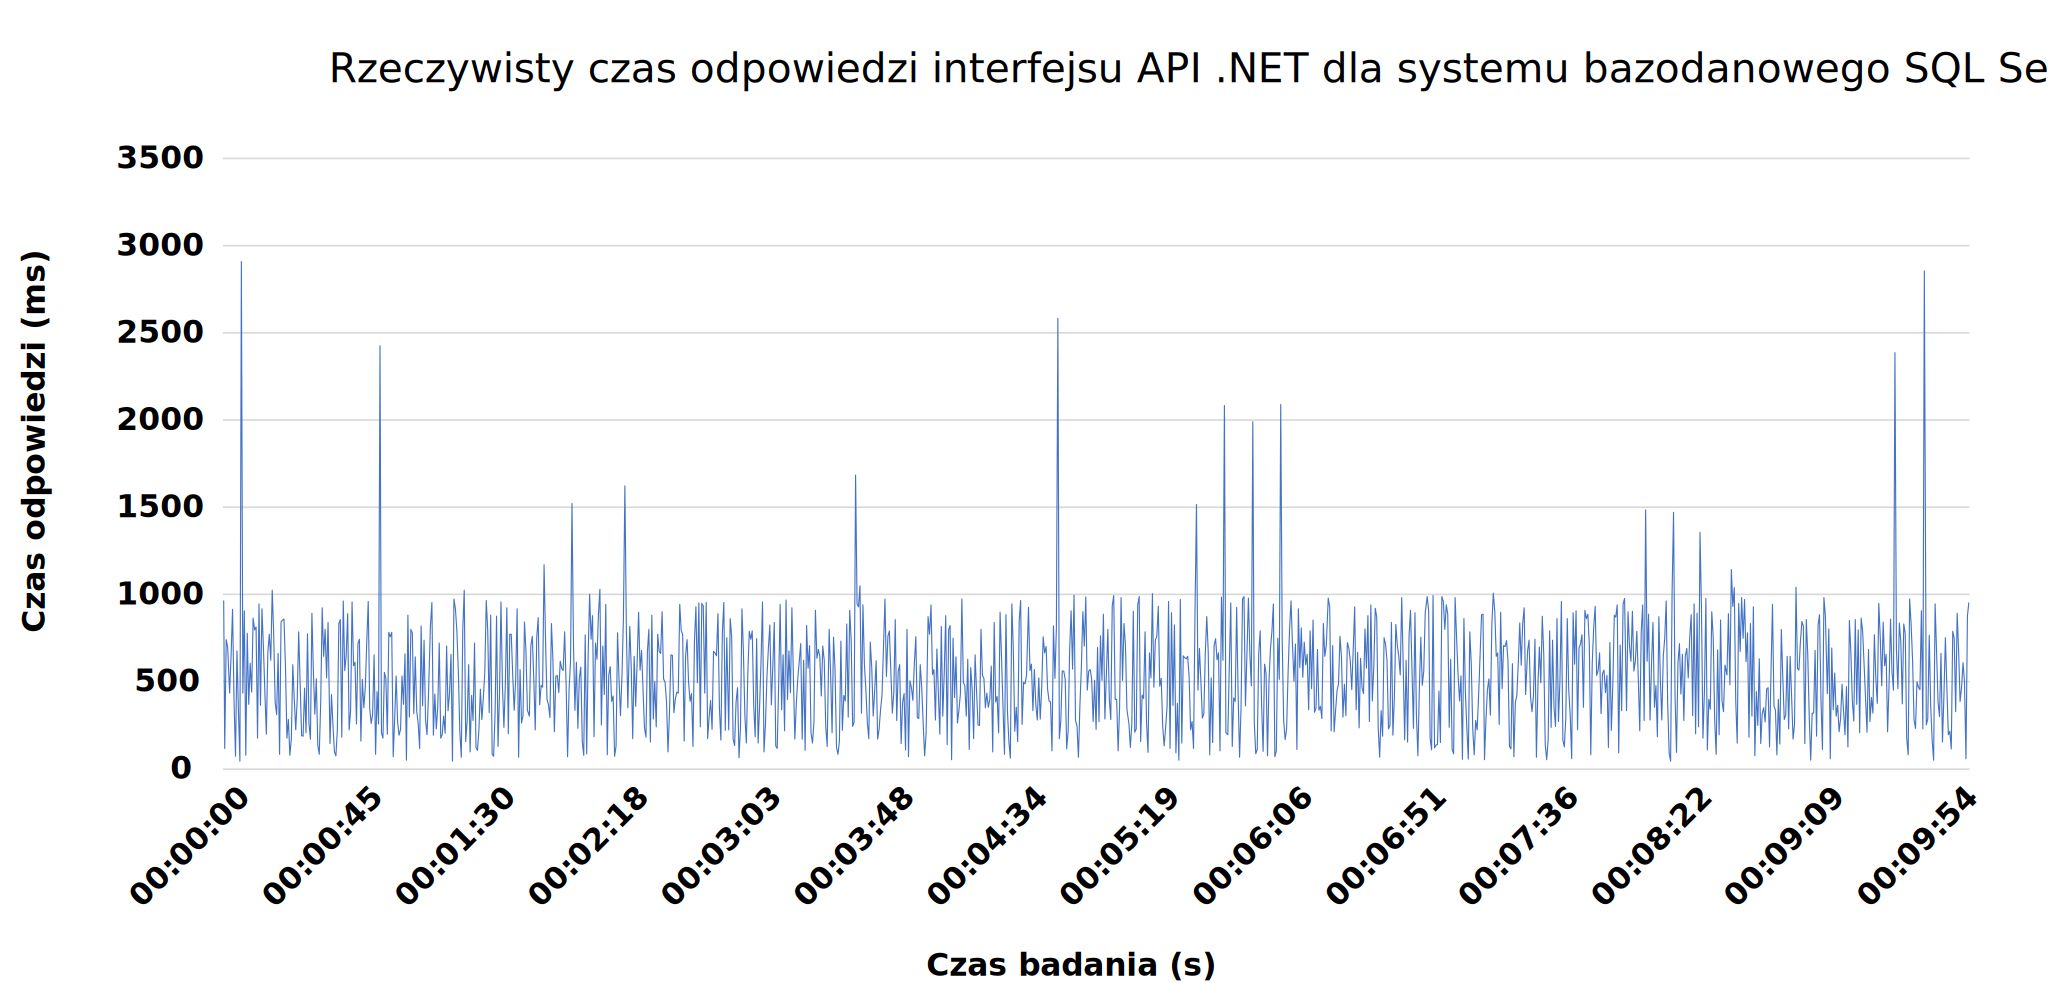
\includegraphics[width=\linewidth]{rys05/testy-funkcjonalne-dotnet.pdf}
    \caption{Czas odpowiedzi na żądanie dla konfiguracji .NET/SQL Server w kontekście testu funkcjonalnego}
    \label{fig:wykres-testy-funkcjonalne-dotnet}
\end{figure}

Na podstawie uzyskanych danych, zdefiniowano progi tolerancji oraz frustracji, wykorzystywane jako punkty odniesienia przy kalkulacji wartości wskaźnika APDEX. Wartości te, ustalono poprzez rosnące posortowanie zbioru czasów odpowiedzi API, a następnie symetryczny podział dwupunktowy. Operacja wykonana została dla każdego z porównywanych systemów bazodanowych w obrębie obu technologii implementacyjnych dotyczących interfejsów API.

Uzyskane przedziały satysfakcji, tolerancji oraz frustracji względem każdego systemu bazodanowego oraz technologii tworzenia API zostały zobrazowane na wykresach \ref{fig:apdex-dotnet} oraz \ref{fig:apdex-nodejs}.

\begin{figure}[ht]
    \centering
     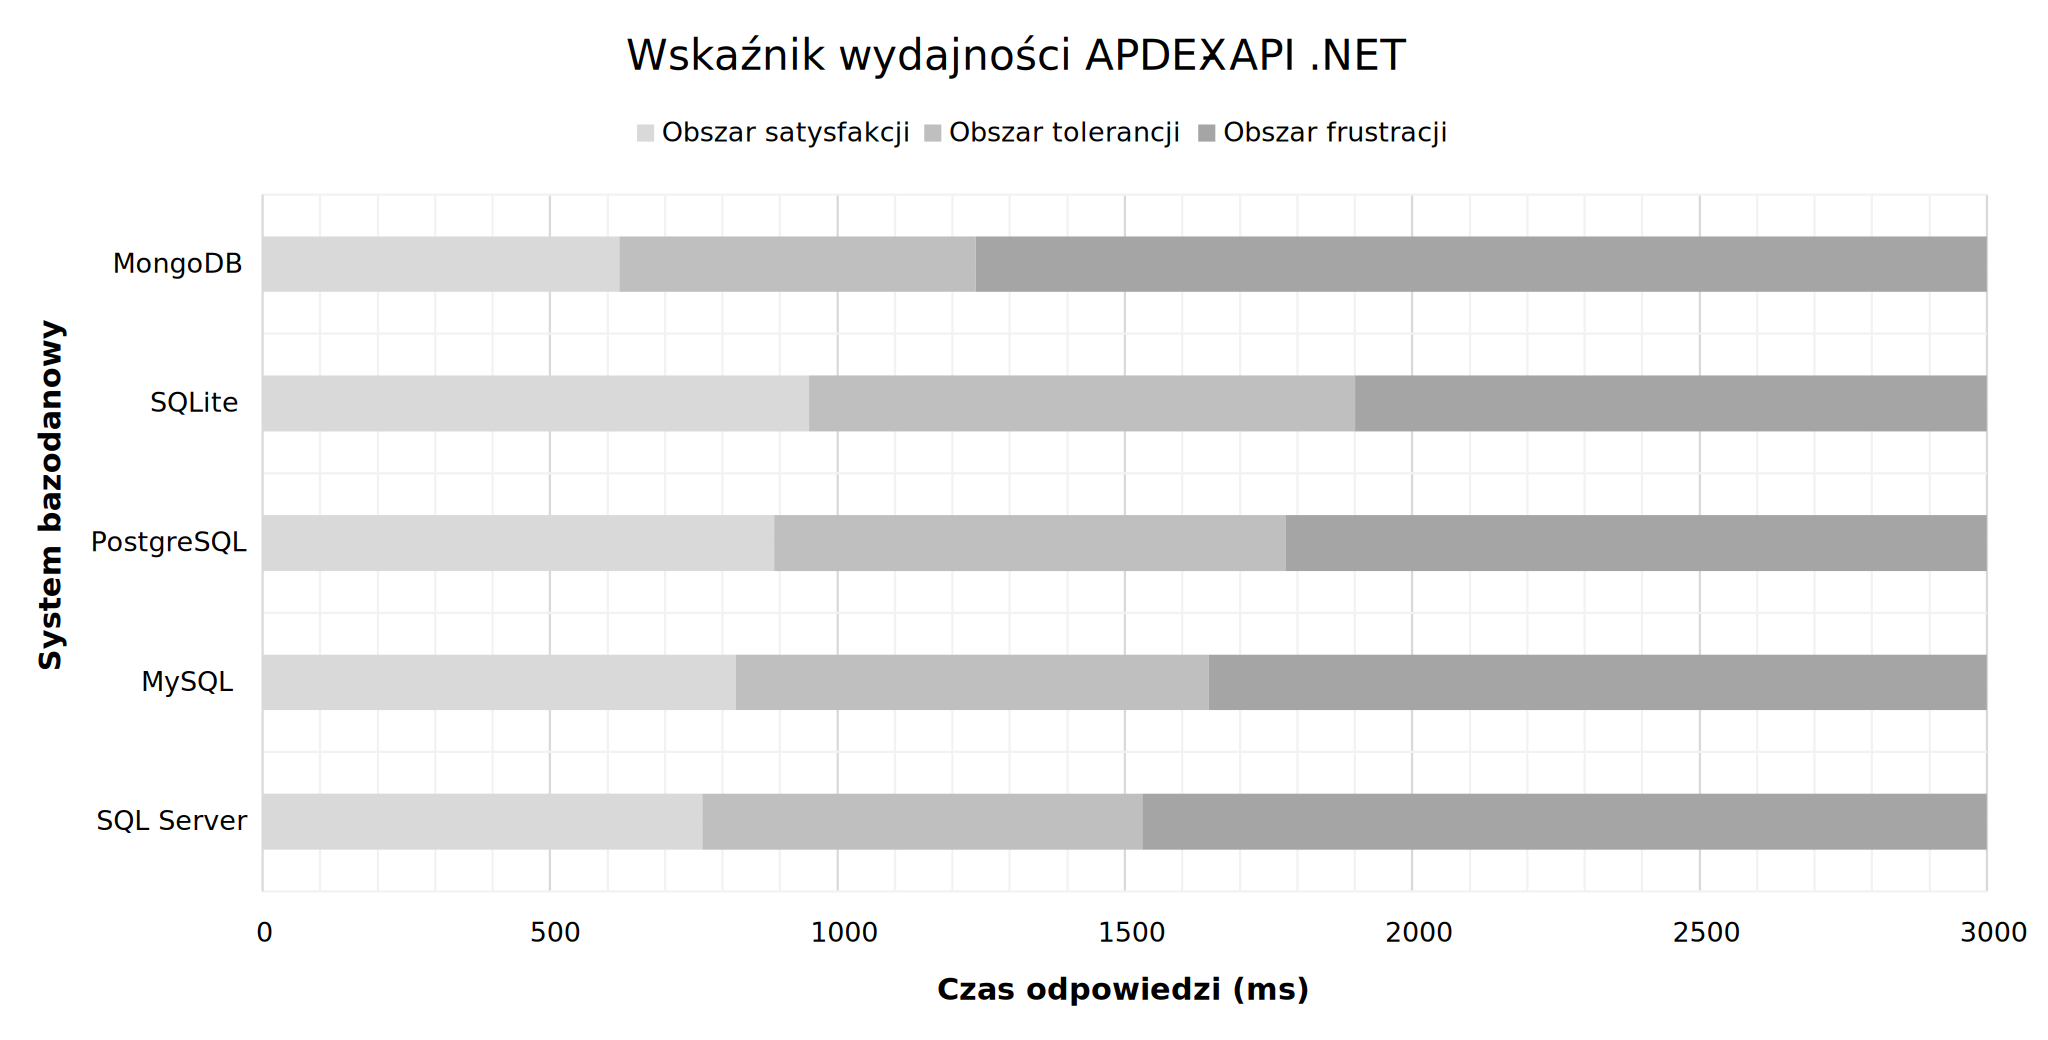
\includegraphics[width=\linewidth]{rys05/apdex-dotnet.pdf}
    \caption{Obszary satysfakcji, tolerancji oraz frustracji wskaźnika APDEX względem poszczególnych systemów bazodanowych dla API zaimplementowanego w C\#}
    \label{fig:apdex-dotnet}
\end{figure}

\begin{figure}[ht]
    \centering
     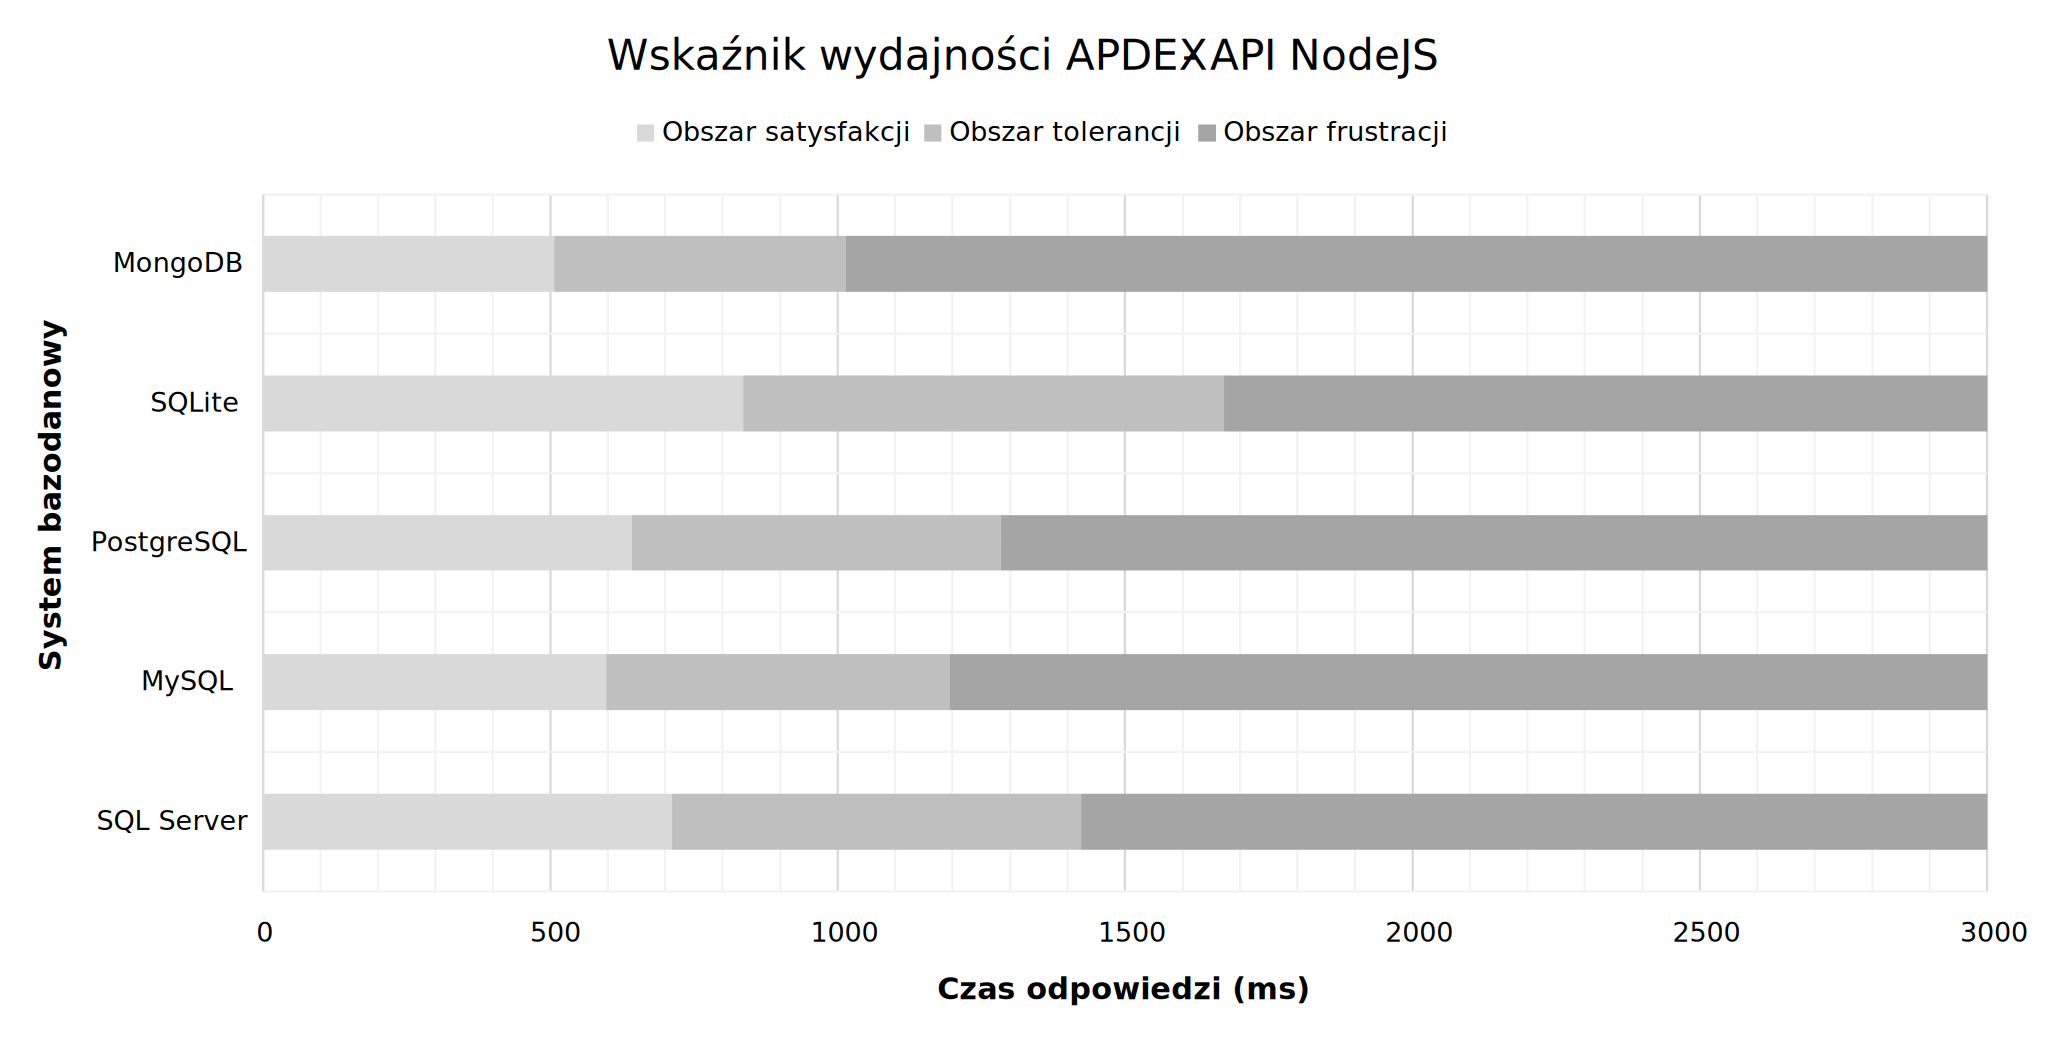
\includegraphics[width=\linewidth]{rys05/apdex-nodejs.pdf}
    \caption{Obszary satysfakcji, tolerancji oraz frustracji wskaźnika APDEX względem poszczególnych systemów bazodanowych dla API zaimplementowanego w JavaScript}
    \label{fig:apdex-nodejs}
\end{figure}

\section{Wpływ zastosowanej technologii programistycznej na wydajność realizacji operacji współbieżnych}
\section{Wpływ zastosowanej technologii programistycznej na efektywność obsługi operacji asynchronicznych}
\section{Wpływ implementacji wzorca projektowego podziału odpowiedzialności na wydajność obsługi żądania klienta}
\section{Porównanie efektywności obsługi żądań klienckich w stałym czasie z uwzględnieniem odmienneych implementacji mechanizmów pamięci podręcznej}
\section{Zmienność wydajności interfejsu API wdrożonego na generycznej oraz dedykowanej platformie chmurowej}
\chapter{Podsumowanie}
\section{Uzyskane efekty pracy}
Celem niniejszej pracy była ewaluacja wydajności interfejsów programowania aplikacji implementowanych w dwóch różnych technologiach, w odniesieniu do licznych aspektów dotyczących sposobów ich wykorzystania. Zdecydowano się nie tylko na analizę efektywności podstawowych rodzajów operacji protokołu hipertekstowego, wchodzących w skład tak popularnych dzisiaj usług sieciowych, ale także wykorzystania mechanizmów programowania współbieżnego, technik obsługi żądań asynchronicznych, implementacji zaawansowanego wzorca projektowego, zastosowania rozwiniętych technik optymalizacji pozyskiwania danych, a także wdrożenia rozwiązań w kontekście środowisk chmurowych.

Zwrócenie uwagi na tak wiele aspektów dotyczących interfejsów programowania aplikacji miało na celu uświadomienie czytelnika, że tego typu systemy internetowe, wykorzystywane są powszechnie nie tylko do realizacji najpopularniejszych czterech, podstawowych operacji na danych. Wachlarz możliwości związanych z tworzeniem internetowych API jest znacząco szerszy, a fakt ten uwydatnia się wraz z rosnącym poziomem skomplikowania usług sieciowych, a także zadań, które są przed nimi stawiane.

Zastosowanie mnogości kontekstów, w których odnaleźć musiały się przygotowane rozwiązania miało również odmienny cel. Misją autora było dowiedzenie się czy którykolwiek z systemów opartych o dwie porównywane technologie wdrożeniowo-uruchomieniowe, wykazuje wysoką wydajność względem swojego konkurenta w którymkolwiek z obszarów prowadzonych badań. Jeżeli tak, to które z tych obszarów są faworyzowane przez konkretne technologie.

Wyniki przeprowadzonych badań umożliwiły rozwianie powyższych wątpliwości, a także uzyskanie dodatkowej wiedzy, która nawet dla osób posiadających doświadczenie w zakresie kompozycji oraz tworzenia interfejsów API nie musi wydawać się oczywista. Zrealizowane eksperymenty uwidoczniły niektóre zależności, zadając innym z kolei kłam. Przykładem potwierdzenia spodziewanej hipotezy, może być wykazana wyższość wydajności rozwiązań implementowanych na platformach dedykowanych względem platform generycznych. Kolejną egzemplifikacją, w ramach której, jeszcze przed przeprowadzeniem badania, sformułować można było silną hipotezę, była obserwacja wpływu zastosowania usprawnień wydajnościowych, separacji środowisk bazodanowych, a także wdrożenia wzorca podziału odpowiedzialności. Rezultaty badania systemów bazodanowych z kolei, mogą być doskonałym argumentem, na obalenie hipotezy wyższej efektywności komunikacji silników baz danych oraz interfejsów tworzonych na bazie technologii jednego producenta.

Odnosząc się do dodatkowej wiedzy, której chęć pozyskiwania wzmożona została poprzez ambicję wyjaśnienia pojawiających się w badaniach anomalii, wspomnieć należy o sposobie obsługi wielowątkowej w odniesieniu do współbieżnie generowanych, długotrwających żądań. Obsługa ta niemalże nie występuje w kontekście interfejsu języka JavaScript, natomiast jest wydatnie rozbudowana w przypadku usługi implementowanej w C\# i uruchamianej na platformie .NET. Ponadto ciekawym jest również fakt, jak bardzo prostota, tycząca się mechanizmów wywoływania operacji asynchronicznych, może nieść korzyść dotyczącą wydajności ich realizacji.

W niektórych przypadkach jednak konwencjonalność rozwiązania nie idzie w parze z jego wydajnością. Potwierdzeniem tego właśnie stwierdzenia są przeprowadzone badania dotyczące podstawowego oraz autorskiego podejścia do realizacji mechanizmów pamięci podręcznej. W ramach pracy tej, zaimplementowano, a także zbadano zachowanie systemu cache uwzględniającego częstotliwość wywoływania punktu końcowego, a także liczbę unieważnień identyfikującego go wpisu. Zgromadzone rezultaty należy postrzegać jako obiecujące, jednakże wymagana jest zdecydowanie bardzej obszerna analiza uwzględniająca zmienność liczby momentów unieważnień, czy też wpływ dysproporcji parametrów w różnych chwilach obsługi żądań.

Wspomnieć należy również o przeprowadzonych w ramach niniejszego badania parowych testach statystycznych, które pozwoliły na wykazanie statystycznie istotnej przewagi określonych konfiguracji rozwiązań względem pozostałych z nich. 

Bardzo ważnym jest również uwypuklenie pewnej tezy. Przeprowadzony zestaw badań nie wskazał, jednakże przede wszystkim nie miał wskazać, technologii niezaprzeczalnie lepszej. Technologia taka nie istnieje, a wynika to w głównej mierze z ilości obszarów, w kontekście których może ona zostać wykorzystana oraz badana. Dlatego też, dokument ten, może okazać się pomocny dla tych osób, którzy zainteresowani są oceną poziomu wydajności interfejsu dla konkretnej technologii oraz konkretnego sposobu jej wykorzystania.
\section{Perspektywy rozwoju badań}
Każdy z przytoczonych obszarów wykorzystania interfejsów programowania aplikacji, reprezentowany w niniejszej pracy poprzez odmienne badanie, może zostać z łatwością rozbudowany poprzez ewaluację dodatkowych metryk wydajnościowych, czy też zmianę konfiguracji środowiska badawczego. Zdecydowano się na wskazanie perspektyw rozwoju badań w odniesieniu do tych domen funkcjonalności API, które zostały poruszone w tym dokumencie.

Odwołując się do badania wpływu wykorzystania systemów bazodanowych w kontekście porównywanych technologii, jako perspektywę rozwoju wskazać należy przeprowadzenie ewaluacji wydajności dla przedziałów liczby wątków-generatorów o zmiennej długości. Ponadto, wzięte pod uwagę mogą być również te spośród systemów bazodanowych, w ramach których nie dostarczane jest wsparcie dla mapperów obiektowo-relacyjnych Entity Framework Core oraz Prisma.

W ramach badania realizacji operacji współbieżnych, wprowadzić można dodatkowe rodzaje algorytmów metaheurystycznych dla różnych problemów o wysokiej złożoności obliczeniowej. Interesującą perspektywą rozwoju tego badania, jest również implementacja odmiennych heurystyk dla symetrycznego problemu komiwojażera, a także porównanie ich wykonania dla interfejsów wspierających przetwarzanie wielowątkowe.

Badanie wydajności operacji asynchronicznych może zostać poszerzone o uwzględnienie różnych implementacji klientów protokołu hipertekstowego, a także konfiguracji poszczególnych ich parametrów.

Najwięcej perspektyw rozwoju badań, wyróżnić należy w kontekście ewaluacji porównywanych mechanizmów pamięci podręcznej. Zbadane mogą zostać między innymi odmienne metryki wpływające na zmianę czasu odpowiedzi na żądanie. Jako przykładową metrykę wskazać można narzut wydajnościowy wprowadzany przez metodę kalkulacji czasu życia wpisu w magazynie pamięci podręcznej. Ponadto, struktura wykonanego badania, mogłaby zostać dostosowana względem zmiennego czasu trwania testu, zmiennego natężenia ruchu sieciowego, czy też deterministycznego charakteru wywoływania żądań unieważniających. Co więcej, zaproponowana przez autora metoda może zostać zmodyfikowana poprzez uzależnienie czasu przechowywania wpisu od dodatkowych parametrów, bądź też zmianę ich istotności względem wyliczania czasu życia elementu pamięci cache.

W kontekście wprowadzenia wzorca podziału odpowiedzialności, a także separacji modeli bazodanowych, badanie może zostać poszerzone o zastosowanie odmiennych mechanizmów replikacji, niż wykorzystana w tej pracy technika transakcyjna. W takim przypadku, należy zbadać w jakim czasie, od momentu dodania rekordu bazodanowego, będzie on dostępny w ramach źródła danych przeznaczonego do odczytu. Co więcej, należy pamiętać, że celem zdefiniowania specyficznej struktury obsługi żądania, była możliwość optymalizacji modeli danych. Dlatego też, interesującą perspektywą rozwoju tego badania, mogłoby być wskazanie, które z zaimplementowanych technik optymalizacji mają kluczowe znaczenie pod kątem wydajności, a które wpływają na nią jedynie nieznacznie.

Ostatnie ze zidentyfikowanych perspektyw rozwoju tyczą się obserwacji efektywności działania w odniesieniu do produkcyjnych środowisk chmurowych. Biorąc pod uwagę ten właśnie aspekt, możliwym jest dokonanie porównania dla większej liczby platform wdrożeniowych, czy też zbadanie, w jaki sposób usługi generyczne typu infrastructure-as-a-service mogą zostać zoptymalizowane, aby implementowane wewnątrz nich systemy internetowe, osiągały wydajność przybliżoną, lub wyższą względem rozwiązań dedykowanych. 


%\bibliographystyle{plalpha}
\bibliographystyle{plabbrv}

%UWAGA: bibliotek referencji naley przygotowa samemu. Dobrym do tego narzdziem jest JabRef.
%       Nazw przygotowanej biblioteki wpisuje si poniej bez rozszerzenia 
%       (w tym przypadku jest to "dokumentacja.bib")
\setlength{\bibitemsep}{2pt} % - by zacieni wykaz literatury
%\addtocontents{toc}{\addvspace{5pt}} % ustawiamy odstp przed literatur w spisie treci
\bibliography{dokumentacja}
\appendix
\chapter{Instrukcja wdroeniowa}
Jeli praca skoczya si wykonaniem jakiego oprogramowania, to w dodatku powinna pojawi si instrukcja wdroeniowa (o tym jak skompilowa/zainstalowa to oprogramowanie).
Przydaoby si rwnie  krtkie how to (jak uruchomi system i co w nim zrobi -- zademonstrowane na jakim najprostszym przypadku uycia). Mona z tego zrobi osobny dodatek,
\chapter{Opis zaczonej pyty CD/DVD}
Tutaj jest miejsce na zamieszczenie opisu zawartoci zaczonej pyty.
Naley wymieni, co zawiera.

% Ponisze jest niepotrzebne, jeli nie generuje si indeksu
%%\chapterstyle{noNumbered}
%%\phantomsection % sets an anchor
%%\addcontentsline{toc}{chapter}{Indeks rzeczowy}
%%\printindex

\end{document}
